% !TEX TS-program = pdflatex
\documentclass[preprint,showpacs,aps,prc,superscriptaddress]{revtex4-1}
\usepackage{amsfonts}
\usepackage{amsmath}
\usepackage{txfonts}
\usepackage{amssymb}
\usepackage{mathrsfs}
\usepackage{graphicx}
\usepackage{dcolumn}
\usepackage{lineno}
\usepackage{hyperref}
\usepackage{multirow}
\usepackage{epstopdf}
\usepackage{natbib}
\usepackage{subfigure}
%\usepackage{tocloft}
%\setlength{\cftpartnumwidth}{3em}
%\def\l@section{\@dottedtocline{1}{2em}{2em}}
\renewcommand\thesection{\arabic{section}}
\renewcommand\thesubsection{\arabic{section}.\arabic{subsection}}
\renewcommand\thesubsubsection{\arabic{section}.\arabic{subsection}.\arabic{subsubsection}}
%arabic 阿拉伯数字 
%roman 小写的罗马数字 
%Roman 大写的罗马数字 
%alph 小写字母 
%Alph 大写字母
\hypersetup
{
    CJKbookmarks=true,
    bookmarksnumbered=true,
    bookmarksopen=true,
    breaklinks=true,
    colorlinks=true,
    linkcolor=blue,
    citecolor=blue,
    plainpages=false,
    pdfstartview=FitH
}
\newcommand{\snn}{\sqrt{s_\text{NN}}}
\newcommand{\pt}{p_T}
\newcommand{\gc}{GeV/$c$\ }
\newcommand{\bv}[1]{\textbf{\emph{{}#1}}}
\newcommand{\ffps}[1]{E_{{}#1}\frac{d^3\bv{N}_{{}#1}}{d\bv{p}^3_{{}#1}}}
\newcommand{\sfps}[1]{\frac{d^6\bv{N}_{{}#1}}{d\bv{r}^3_{{}#1}d\bv{p}^3_{{}#1}}}
\newcommand{\tfps}[1]{\frac{d^3\bv{N}_{{}#1}}{d\bv{p}^3_{{}#1}}}
\newcommand{\npart}{\langle N_{\textrm{part}}\rangle}

\begin{document}
\preprint{}

\title{
\Huge{Analysis Note: \\ \textbf{Identified particle flow measurements in Au+Au collisions at $\sqrt{s_{NN}}$ = 3 GeV from RHIC-STAR}}
}
%\author{Shaowei Lan}
\email[]{shaoweilan@mails.ccnu.edu.cn}
%\affiliation{Key Laboratory of Quark $\&$ Lepton Physics (MOE) and Institute of Particle Physics, Central China Normal University, Wuhan, 430079, China}
%\date{\today \ \ \ Version 1.0}


\begin{abstract}

\noindent\rule[0.25\baselineskip]{\textwidth}{1pt}
Collectivity is a powerful tool for understanding the properties of the medium created in high-energy nucleai collisions. In this note we report the rapidity(y) dependence of azimuthally anisotropic parameters ($\rm v_{1}$ and $\rm v_{2}$) for identified hadrons ($\pi^{\pm}, K^{\pm}, K_{S}^{0}, p, \phi, \Lambda$) from Au+Au collisions at a center-of-mass-energy per nuclean pair ($\sqrt{s_{NN}}$) of 3 GeV. These results are compared with that from high collision energy $\sqrt{s_{NN}}$ $>$ 4.5 GeV. It is found that at this energy in the 10-40\% mid-central collisions (1) the midrapidity slopes $dv_{1}/dy|_{y=0}$ for all hadrons are positive except pions; (2) the midrapidity elliptic flow $v_{2}$ are all negative and the number of consistent quark scaling, observed in high energy collision is absent. These observations imply new medium properties produced that are different from the partonic matter created in high energy collisions.
%\noindent\rule[0.25\baselineskip]{\textwidth}{1pt}
\end{abstract}

\maketitle
\listoffigures
\listoftables
\tableofcontents
%\makeatletter
%\let\toc@pre\relax
%\let\toc@post\relax
%\makeatother

\newpage


\linenumbers
\section{Analysis Setup}
In this section, we mainly discuss the setup of our analysis. We will introduce the conventions of fixed target collision mode, and the bad run selection from run-by-run QA.
We will also discuss the data sets and the event and track cut we used in this analysis. Finally, the centrality determination will be discussed.
\subsection{Fixed Target Conventions}
In the year 2018, STAR collected fixed-target mode data, the center of mass energy $\sqrt{s_{NN}}$ is 3 GeV (beam energy of 3.85 GeV/u). For the fixed target mode collisions, It is not same as collider mode, the lab frame and the center of mass frame are not same, the midrapidity is not 0. For example, to define the mid-rapidity, we need to boost the measured rapidity in the lab frame into center of mass frame. The midrapidity is half of beam rapidity, beam rapidity can be calculated from this equation.

\begin{figure}
    \centering
    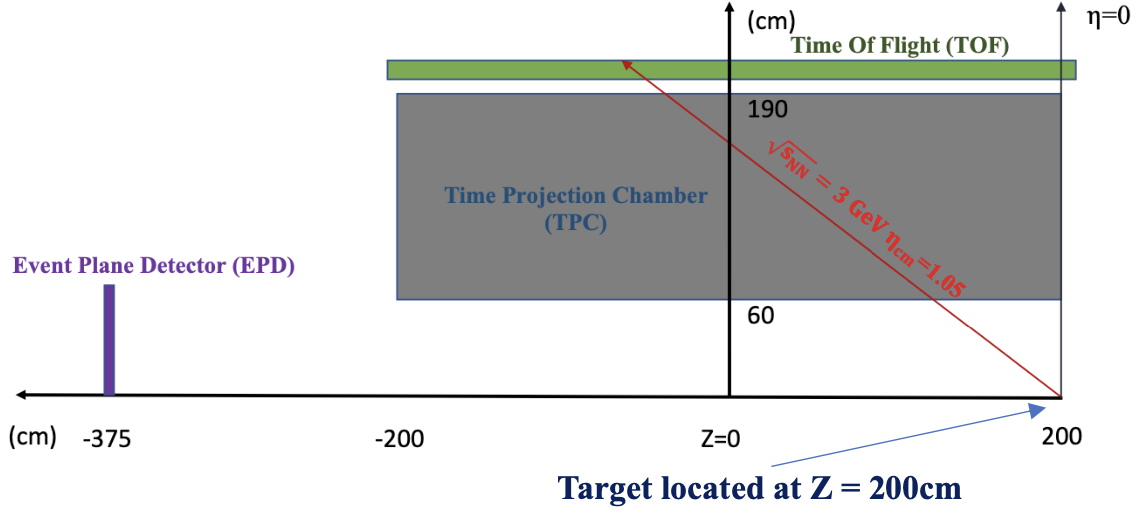
\includegraphics[scale=0.5]{FXT3gev/chapter1/fig/FXT_schematic.jpg}
    \caption{The schematic plot for fixed target collision}
    \label{fig:FXT_schematic}
\end{figure}

\begin{equation}
	y_{b} = cosh^{-1} \left[ \frac{\sqrt{s_{NN}}}{2*m_{p}} \right]
	\label{beamy_cal}
\end{equation}
Where the $\sqrt{s_{NN}}$ is center of mass energy (3 GeV), the $m_{p}$ is proton mass (0.938). In our STAR convention, the beam-going direction is the positive direction (the target is located in the negative rapidity direction $y_{target}$ = -1.045). In order to match the STAR conventions, when calculating rapidity in center of mass frame, in addition to shift by midrapidity, we also need to flip the sign of rapidity. 
\begin{equation}
	y_{CM} = -(y_{lab}-y_{mid})
	\label{rap_convention}
\end{equation}

Figure \ref{fig:FXT_schematic} shows the schematic plot for fixed target collision. In the STAR coordinate system, the target located at Z=200cm the edge of TPC. The EPD located at -375 cm. Red line indicates $\eta$=1.05 and it is roughly midrapidity region.


\subsection{Datasets and Event Selection cuts}
In this study, we analyze the minimum bias events for Au + Au collisions at $\sqrt{s_{NN}}$ = 3 GeV from Fixed target mode, single beam energy is 3.85 GeV. The trigger information and event selection are summarized in the  TABLE \ref{table1}. Since the target is fixed, in our analysis we set the vertex cut along the Z direction is [198, 202] cm, in the X and Y direction, we set the Vr ($\sqrt{Vx^{2}+Vy^{2}}$) less than 2 cm around (0, -2). The total number of minimum bias events is 310 million, and after event cuts (Vz and Vr cut), we still have 280 million good events.

\begin{table}[h]
\centering
\caption{\ Event cuts and total number of minimum bias events}
\label{table1}
\begin{tabular}{l l l l l l l}
%\begin{tabular}
	\hline
\small{\textbf{Energy($\sqrt{s_{NN}}$ GeV)}} & \small{\textbf{Trigger ID (minimum bias)}} & \textbf{Vz(cm)} & \textbf{Vr((0,-2) cm)} & \textbf{Total Events(M))} & \textbf{Good Events(M)}\\
3.0 & 620052 & [198, 202] &2 & 310 & 280 \\
	\hline
\end{tabular}
\end{table}
 
\subsection{Badrun selection}
Due to the detector performance during the data taking, we need to select the bad runs, which might influence our analysis and results. In our analysis, 7 event and track variables (Vz, Vr, refmult, dca, eta, phi, pt) will be used to select bad runs. With event (Vz and Vr) cut,  we plot each variable's mean value as a function of run index in the figure \ref{fig:bad}, totally there are 191 runs at 3GeV. After applying the event cuts (198 $<$ Vz $<$ 202 cm and Vr $<$2 cm), and we plot these variable' mean value as a function of run index, the run index is corresponding to each run number. The second step, we perform minimum and maximum cut (the blue dash line) for each variable to exclude the extreme data(they are far away from the rest of data point). The third step, we calculate the mean value (red solid line) and 3$\sigma$ (red dash line) of the rest data. After that, we can select the bad runs, which are outside the 3$\sigma$ region. totally we have 21 bad runs, these runs will be removed in this analysis.
	

\begin{figure}[ht]
\centering
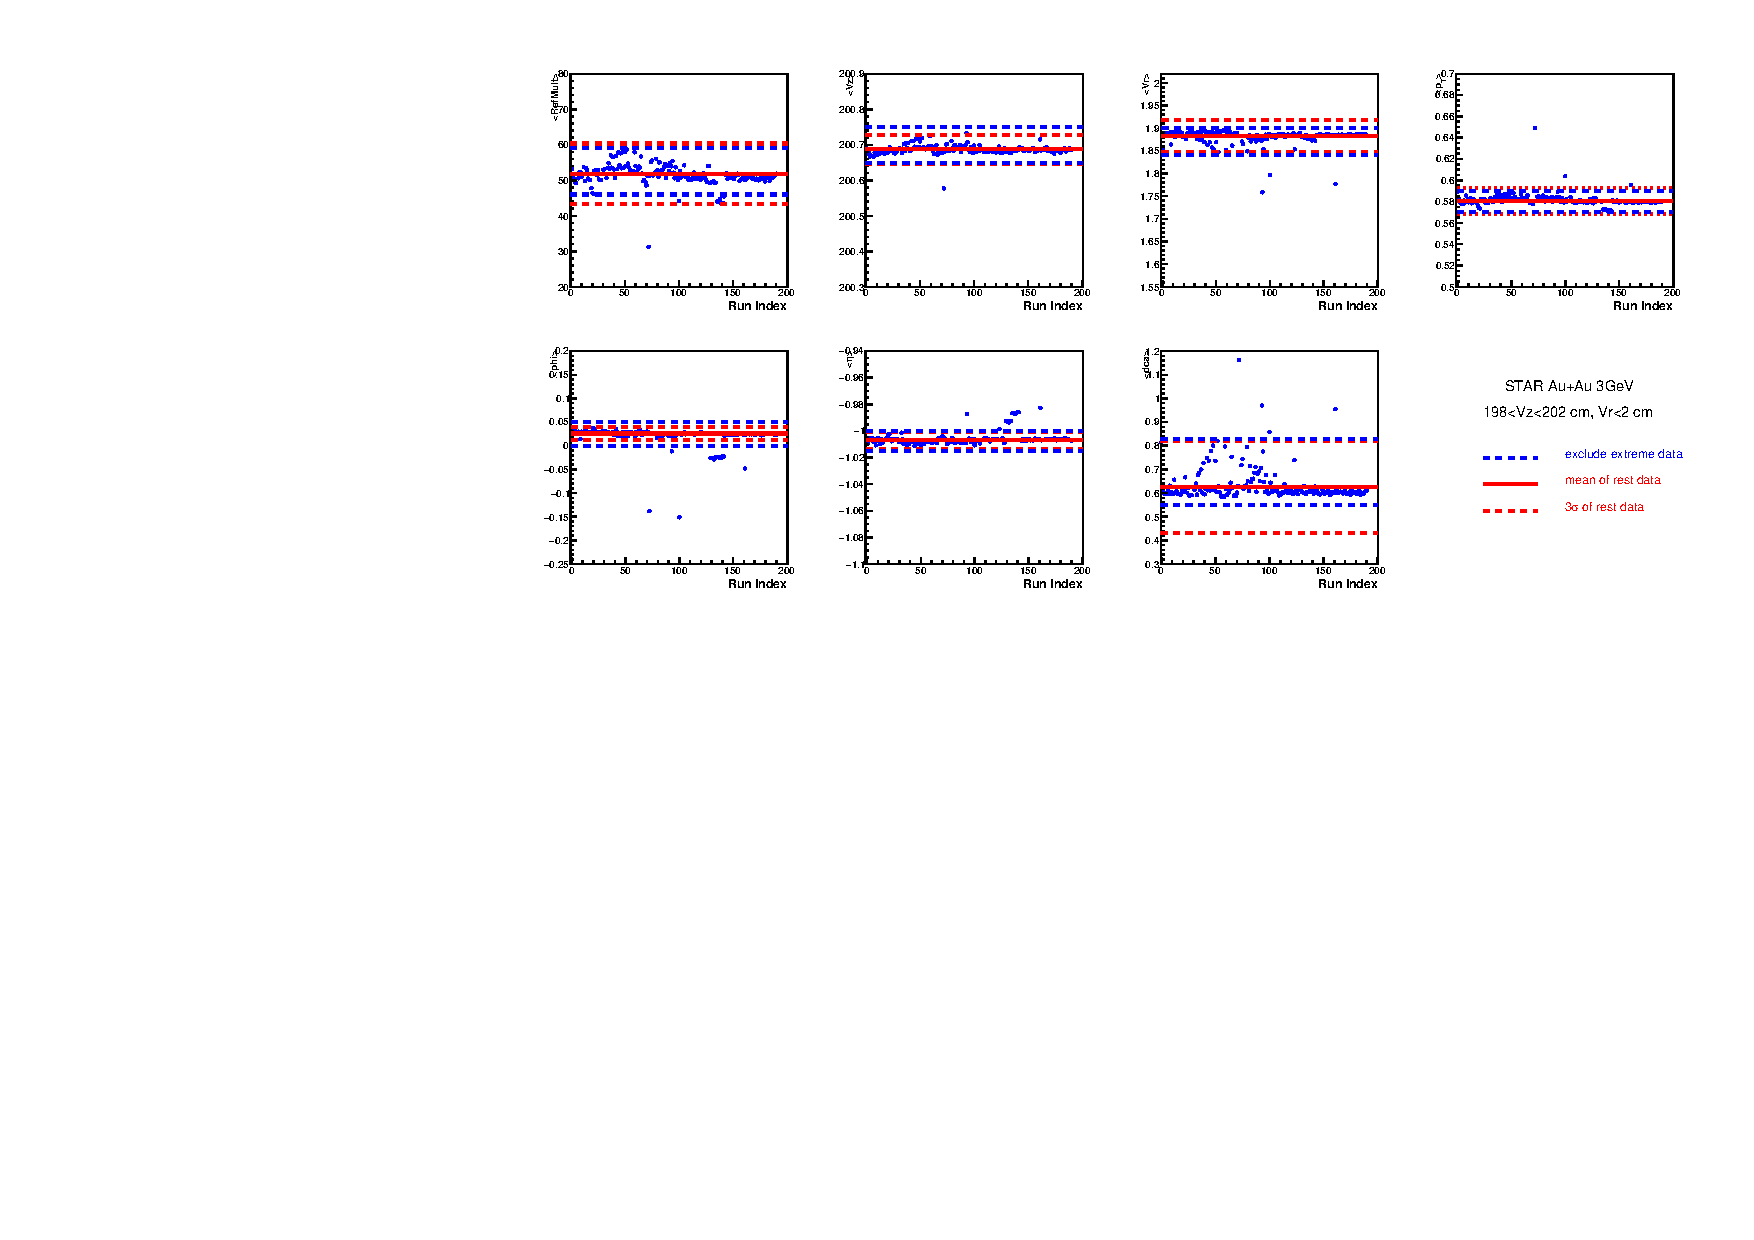
\includegraphics[scale=0.9]{chapter1/fig/badruns.pdf}
\caption{ These variables' (Vz, Vr, refmult, dca, eta, phi, pt) mean value as a function of run index.}
\label{fig:bad}
\end{figure}

From this selection and possible reasons based on shift log in the TABLE \ref{badruns}. The relevant reference could be found at \href{https://drupal.star.bnl.gov/STAR/system/files/Good_run_list_3.85_1.pdf}{Badruns}

\begin{table}[h]
\centering
\caption{\ Bad runs list and what's wrong}
\label{badruns}
\begin{tabular}{cc}
\hline
Bad runs & What's wrong with this run? \\
\hline
\textbf{19151029} & First data run. Fill was with 36 bunches, not 12. \\
\textbf{19152001} & Run has only 1 event.  \\
\textbf{19152078} & 1 minute run, not in the shift log book. \\
\textbf{19153023} & 3.5 minute run, get almost no rate, asked MCR, then TPC trips. \\
\textbf{19153032} & 35 second run, run stopped with TPC trips. \\
\textbf{19153065} & 35 second run, run stopped with two inner TPC trips. \\
\textbf{19154012-19154024} & TPC sector 14 has four RDOs missing. \\
\textbf{19154026} & BTOW is out for this run. \\
\textbf{19154051} & 45 second run, inner TPC tripped during the run. \\
\hline
\end{tabular}
\end{table}


\subsection{Centrality Determination}

Due to the large luminosities at FXT model collisions, more than one collision with the target can happen within the same bunch crossing. It is estimated that there are $\sim$ 1\% of the events and will significantly affect higher moment analyses. In this analysis, the spectator and midrapidity correction is used to consider for pileup events rejection. We can use TPC to measure midrapidity tracks and EPD to measure hits in the forward rapidity region. Detailed information of this method can be found \href{https://drupal.star.bnl.gov/STAR/system/files/PileupFXT3GeV_BulkCorr.pdf}{pileupremove}.

For the centrality definition, we start from uncorrected multiplicity distribution for charged tracks. In order to simulate this distribution, firstly the simulated multiplicity density is calculated using the two component model \cite{Kharzeev:2000ph} with the number of participants $N_{part}$ and number of collision $N_{coll}$ extracted from the Glauber Monte Carlo simulation as formula \ref{equ:two_com}.

\begin{equation}
    \frac{dN_{ch}}{d\eta} = n_{pp} \left [(1-x)\frac{N_{part}}{2} +xN_{coll}\right]
    \label{equ:two_com}
\end{equation}

where the $n_{pp}$ is average multiplicity in minimum-bias p+p collisions and x is the fraction of the hard component. The event-by-event multiplicity fluctuation has been taken into account by convoluting the negative binomial distribution (NBDs) for a given $N_{part}$ and $N_{coll}$. The NBD distribution in multiplicity n has two parameters, $n_{pp}$ and k, and is defined as formula 

\begin{equation}
    P_{NBD}(n_{pp},k;n) = \frac{\Gamma(n+k)}{\Gamma(n+1)\Gamma(k)} \frac{(n_{pp}/k)^{n}}{(n_{pp}/k+1)^{n+k}}
    \label{equ:NBD_dis}
\end{equation}
where the $\Gamma$ is the gamma function. And the parameters $n_{pp}$ and k of NBD distribution are determined using a search method by looping through various combinations of parameters and performing a $\chi^{2}$ test each time until an best $\chi^{2}$ value is found. Figure \ref{fig:glauber_fit} shows the fit from Glauber Monte Carlo simulation on refmult distribution. From the Monte Carlo simulation, the particle multiplicity distribution is integrated to find the multiplicity corresponding to a given percentage of the total inelastic cross section. It can be found in the table \ref{tab:cent_def} shows the refmult cuts for centrality definition. From the figure \ref{fig:glauber_fit}, the data and simulation are matched well in the high multiplicity region due to the high trigger efficiency, while not in the peripheral collisions. By applying the ratio of simulation fit divide data to assume the reweight factor in the peripheral collision to correct the effect from low trigger efficiency due to detector performance, and it will be also used in our analysis. The trigger efficiency is 62\%, due to this low trigger efficiency, we will only perform our result up to 60\% centrality.
We also study the trigger efficiency using URQMD model, in which these event are thrown into detector acceptance. It is consistent with the results from data. Detailed information can be found in this link \href{https://drupal.star.bnl.gov/STAR/system/files/CentralityFXT3GeVBulkCorrPWG.pdf}{triggereffurqmd}.

\begin{figure}
    \centering
    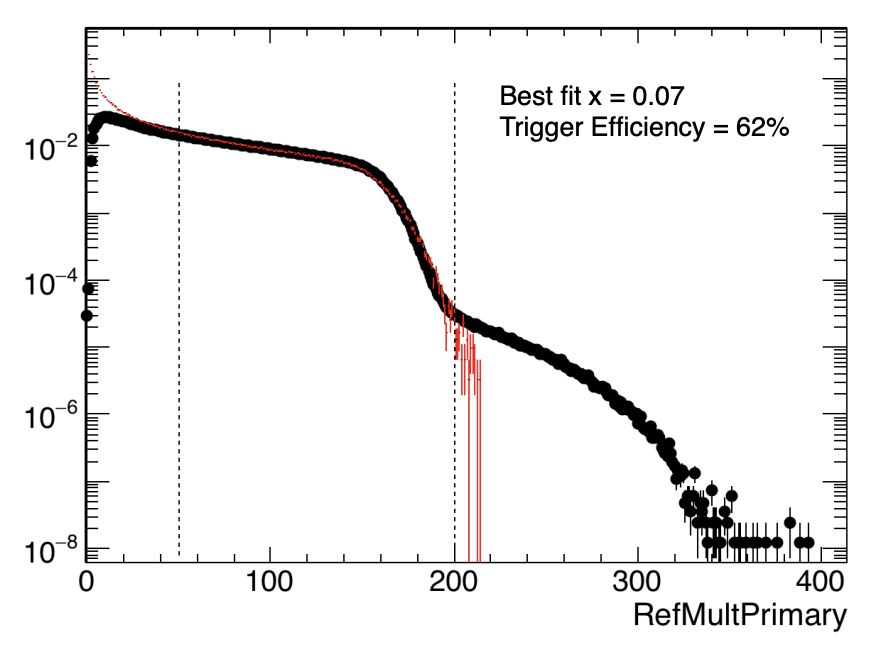
\includegraphics[scale=0.5]{FXT3gev/chapter1/fig/glauber_fit_ref.jpg}
    \caption{Uncorrected refmult distribution measured in the TPC within $|\eta|$ $<$ 0.5 in Au+Au collision at $\sqrt{s_{NN}}$=3GeV. The red line is the fit from Glauber Monte Carlo simulation.}
    \label{fig:glauber_fit}
\end{figure}

\begin{table}[h]
    \centering
    \begin{tabular}{c|c}
    \hline
        centrality & Refmult cut ($>$) \\
        \hline
        0-5\% &  133 \\ 
        5-10\% & 110 \\
        10-15\% & 92 \\
        15-20\% & 76 \\
        20-25\% & 63 \\
        25-30\% & 51 \\
        30-35\% & 42 \\
        35-40\% & 34 \\ 
        40-45\% & 27 \\
        45-50\% & 21 \\
        50-55\% & 16 \\
        55-60\% & 12 \\
        60-65\% & 9 \\
        65-70\% & 6 \\
        70-75\% & 4 \\
        75-80\% & 3 \\
        \hline
    \end{tabular}
    \caption{Refmult cut for centrality definition}
    \label{tab:cent_def}
\end{table}


%Introduction
\clearpage
\section{Analysis Detail}
In this section, we will discuss the analysis detail, in this analysis, the event plane method is used to calculate the directed flow ($v_{1}$)and elliptic flow ($v_{2}$). By following the standard event plane method, firstly we discuss the event plane reconstruction from TPC(Time Projection Chamber) and EPD(Event Plane Detector), TPC's $\eta$ coverage is [-1,1], and the EPD is located at the forward rapidity region, $\eta$ $\in$ (-5.1, -2.1). Since it is Fixed target model collision in this analysis, the acceptance of final state particle is not symmetric around midrapidity, we cannot use 2-sub event method to calculate the resolution, which is commonly used in the BES-I collider model collision, the 2-sub event method requires each sub-event has similar multiplicity and resolution. So, in this analysis, we employ 3-sub event method to calculate the resolution. After that, we will do the particle identification (PID) for pion, kaon proton, then, we introduce the $v_{1}$ and $v_{2}$ calculation.
\subsection{Event Plane Reconstruction}
We will separately introduce the first-order and second-order Event Plane Reconstruction from TPC and EPD.

In order to calculate the resolution for each event plane, we divide the TPC to 2-sub events and EPD to 4-sub events based on their pseudorapidity ($\eta$) range. In the figure \ref{fig:tpc_epd_div}, we show the schematic plot of TPC and EPD sub-events. Since this is fixed-target model collision, we only measure the negative pseudorapidity ($\eta$) region.  In the collider model, the origin point of the Lab frame is in the center of TPC , the EPD is located at $\eta$ $\in$ (-5.1, 2.1). In the fixed-target model, the origin point of the Lab frame is shifted to the edge of TPC, as a result that the $\eta$ of EPD is boosted at $\eta$ $\in$ (-5.3, -2.6).
\begin{figure}[hp]
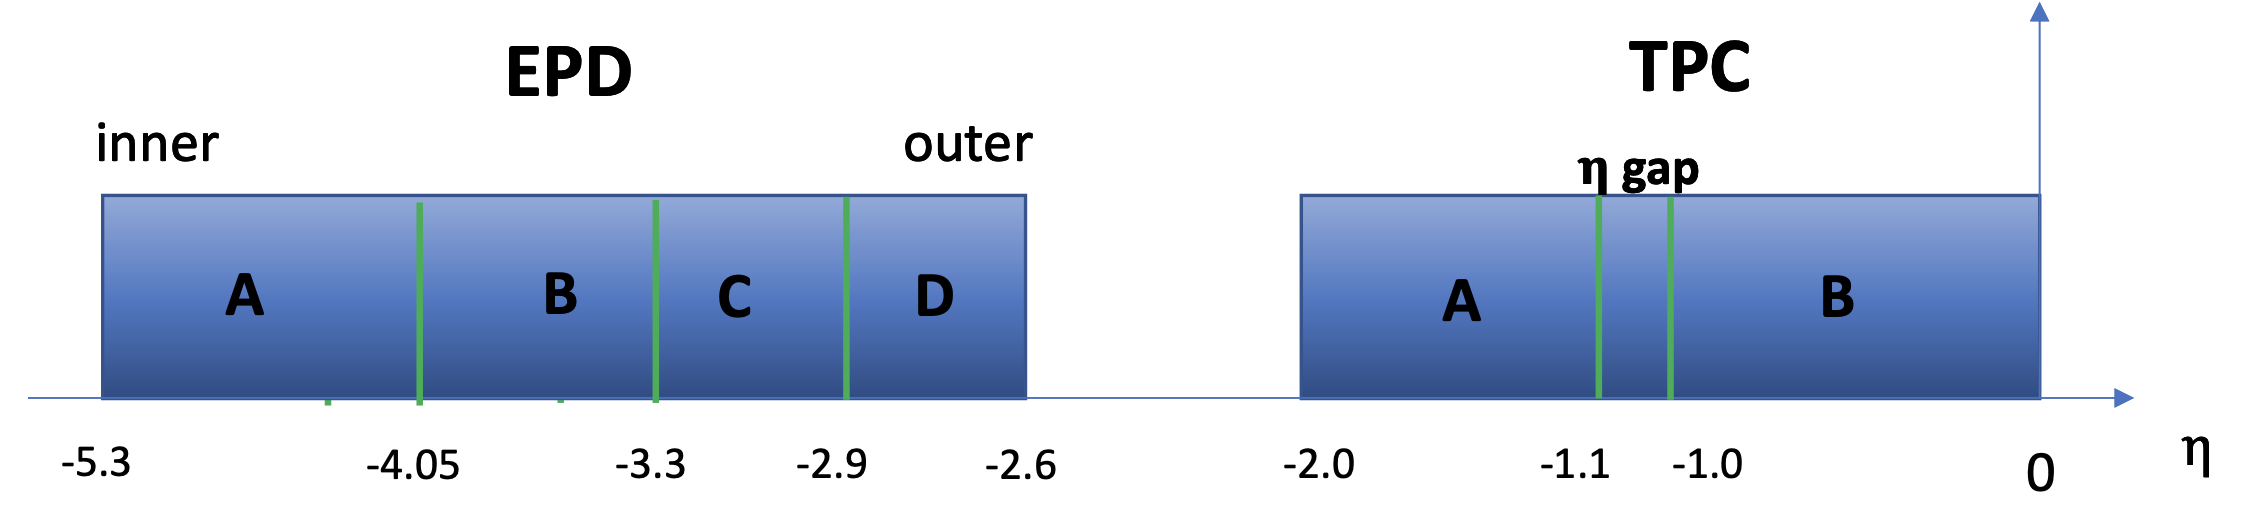
\includegraphics[scale=0.3]{chapter2/fig/tpc_epd_div.png}
\caption{The schematic plot of TPC and EPD sub-events}
\label{fig:tpc_epd_div} 
\end{figure}

\subsubsection{TPC Event Plane Reconstruction}
The event plane method correlates each particle with the event plane determined from these particles without the particle of interest, which can be done for each harmonic. Here we only discuss the first-order event plane reconstruction.
For TPC event plane, these tracks, that are required to pass the following cuts in the table \ref{tab:tpc_ep_cuts}, will be used:
\begin{table}[ht]
\caption{\ Tracks cuts for TPC event plane reconstruction}
\label{tab:tpc_ep_cuts}
\begin{tabular}{|c|c|}
\hline
-2.0$<$ $\eta$ $<$-1.1 (for TPC-A) \\ \hline
-1.0$<$ $\eta$ $<$0 (for TPC-B) \\ \hline
nHitsFit$>$15 \\ \hline
nHitsFit/nHitsMax$>$0.52 \\ \hline
dca $<$ 3 (cm) \\ \hline
0.2 $<$ $p_{T}$ $<$ 2.0 (GeV/c)\\ \hline
\end{tabular}
\end{table}
In order to calculate the first-order event plane angle, firstly we construct the Q vector from particle's azimuthal angle. And the event plane angle can be determined from the Q vector.
\begin{equation}
	\vec{\rm Q}=
	\left( \begin{array}{ccc}
		Q_{y} \\
		Q_{x}
	\end{array} \right)
	=
	\left( \begin{array}{ccc}
		\sum_{i}w_{i}sin(\phi) \\
		\sum_{i}w_{i}cos(\phi)
	\end{array} \right)
	\label{equ:Qvector}
\end{equation}

\begin{equation}
	\Psi_{1} = tan^{-1} \left( \frac{\sum_{i}w_{i}sin(\phi)}{\sum_{i}w_{i}cos(\phi)} \right)
	\label{equ:psi1_TPC}
\end{equation}

\begin{equation}
	w_{i} = 
	\begin{cases}
		p_{T}, 0.2<p_{T}<2.0 (GeV/c) \\
		2.0, p_{T} > 2.0 (GeV/c)
	\end{cases}
	\label{equ:weight_TPC}
\end{equation}

Where sums extend over all particles i used in the event plane calculation, and $\phi$ is particle azimuthal angle in the laboratory frame, and $w_{i}$ is the weight for the $i^{th}$ particle, here we use the $p_{T}$ as the weight and set the threshold of 2GeV in order to suppress the non-flow contribution on event plane reconstruction. The $\Psi_{1}$ is the first-order event plane angle. The reaction plane azimuthal angle distribution should be isotropic in the laboratory frame if the detectors have ideal acceptance. But the detectors always have non-uniform acceptance. In order to remove the acceptance correlations from the imperfect detector, we must make the event plane angle distribution isotropic or flat. A procedure for flattening the laboratory event plane angle distribution is necessary. In this analysis, we perform the re-centering and shift calibration to make the event plane angle distribution flat, it will be discussed in the following. 
\subsubsection{EPD Event Plane Reconstruction}
The event plane reconstruction using EPD is similar to TPC. While the TPC measures the tracks and EPD measures the ADC (analog-digital converter) value in each sectors. The figure \ref{fig:epd_view} shows the schematic plot of EPD (Event Plane Detector). As we can see, EPD has 16 rings, there are 24 sectors in each ring, while there are 12 sectors in the inner most ring, totally one side EPD has 372 sectors, we can measure the azimuthal angle for each sector.
As we can see, in the figure \ref{fig:epd_view}, we divide the EPD to 4 groups based on the rings. From inner to outer, EPD-A (1-4 ring), EPD-B (5-8 ring), EPD-C (9-12 ring), EPD-D (13-16 ring). We will reconstruct the event plane in these EPD groups separately. 
\begin{figure}[hp]
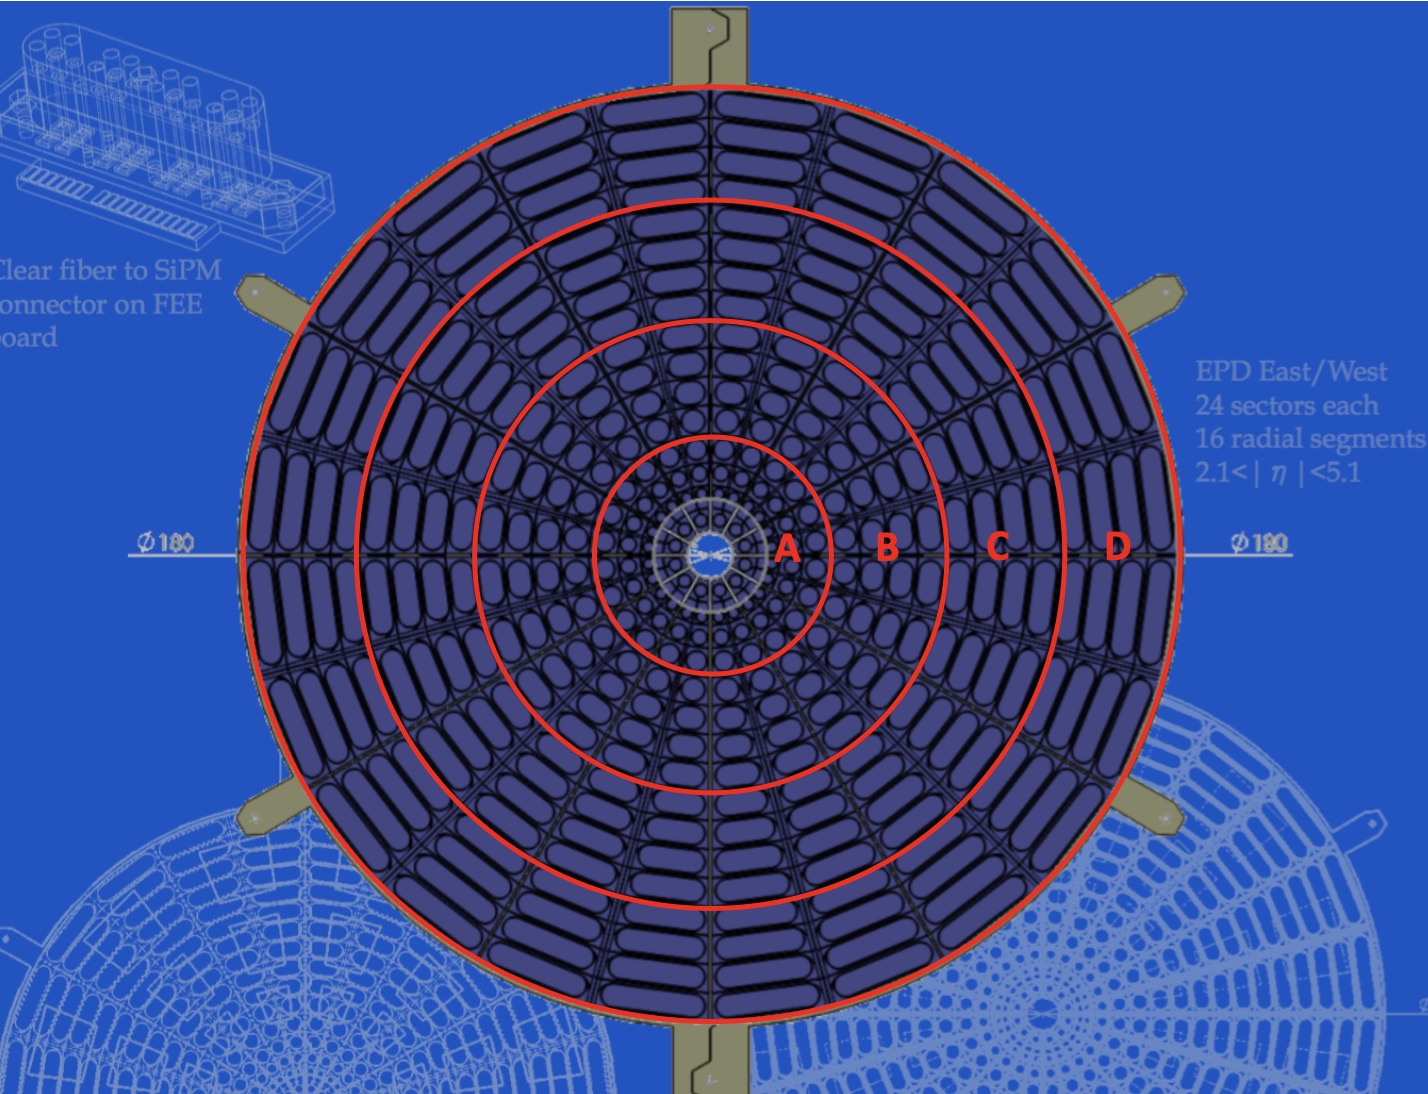
\includegraphics[scale=0.26]{chapter2/fig/epd_div.png}
\caption{The schematic plot of EPD and EPD sub-events}
\label{fig:epd_view} 
\end{figure}

For the event plane reconstruction, we firstly construct the Q vector from the aziluthal angle of sector and calculate the event plane angle from Q vector.
\begin{equation}
	\vec{\rm Q}=
	\left( \begin{array}{ccc}
		Q_{y} \\
		Q_{x}
	\end{array} \right)
	=
	\left( \begin{array}{ccc}
		\sum_{i}w_{i}sin(\phi) \\
		\sum_{i}w_{i}cos(\phi)
	\end{array} \right)
	\label{equ:Qvector_EPD}
\end{equation}

\begin{equation}
	\Psi_{1} = tan^{-1} \left( \frac{\sum_{i}w_{i}sin(\phi)}{\sum_{i}w_{i}cos(\phi)} \right)
	\label{equ:psi1_EPD}
\end{equation}

\begin{equation}
	w_{i} = 
	\begin{cases}
		nMip, 0.3<nMip<2.0 \\
		2.0, nMip > 2.0
	\end{cases}
	\label{equ:weight_EPD}
\end{equation}
Where sums goes over all hits detected by EPD, and $\phi$ is azimuthal angle of EPD sectors in the laboratory frame, and $w_{i}$ is the weight for the $i^{th}$ hits, here we use the nMip as the weight, which is the calibrated ADC value. The $\Psi_{1}$ is the first-order event plane angle. As we discussed before, we will also consider the acceptance correlations from the imperfect detector and  perform re-centering and shift calibration to make the event plane angle distribution flat. In the figure \ref{fig:epd_phi_eta_dis}, we show the EPD azimuthal angle $\phi$ and pseudorapidity $\eta$ distribution using two styles, which means 1: the $\phi$ and $\eta$ in the center position of the corresponding tile. 2: the $\phi$ and $\eta$ value in the random position of the corresponding tile. Although the two styles have different distribution, the results of resolution and $v_{1}$, $v_{2}$ value using two styles are equal.


\begin{figure}[hp]
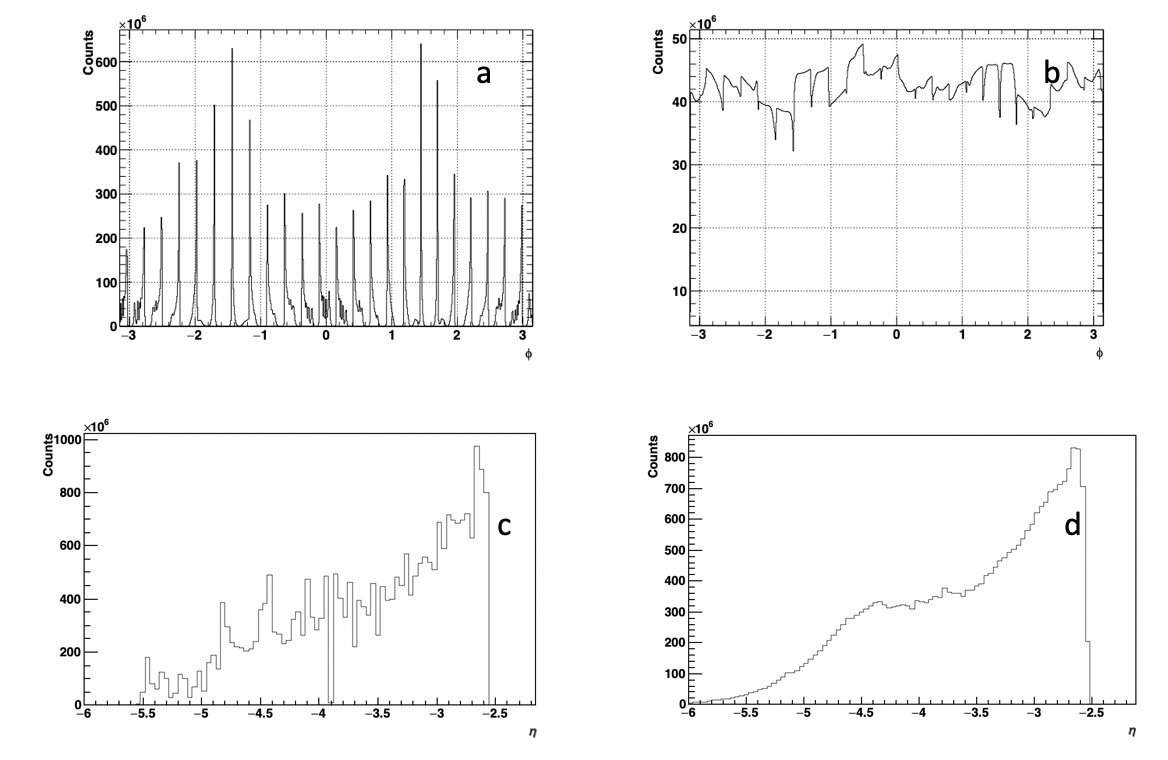
\includegraphics[scale=0.6]{chapter2/fig/epd_phi_eta.png}
\caption{Azimuthal angle ($\phi$) and pseudorapidity ($\eta$) distribution in EPD. (a): $\phi$ distribution in the center of tile, (b): $\phi$ distribution in the random of tile, (c): $\eta$ distribution in the center of tile, (d): $\eta$ distribution in the random of tile}
\label{fig:epd_phi_eta_dis}
\end{figure}

\subsubsection{re-centering and shift calibration}
The re-centering is a track-by-track calibration. One subtracts the factor from the Q-vector of each event, in which the factor is the Q-vector averaged over many events. After that, we can calculate the event plane angle. As we can see in the following equation. It is not enough that we only do the re-centering calibration. We will do the shift calibration further. The shift calibration is that one fits the non-flat distribution of $\Psi_{n}$ averaged over many events with a Fourier expansion and calculates the shifts for each event $\Psi_{n}$ necessary to force a flat distribution on average. The re-centering and shift calibration are all run-by-run and centrality-by-centrality calibration in this analysis.
\begin{equation}
	\vec{Q}_{rc} = 
	\left( \begin{array}{ccc}
	Q_{y, rc} \\
	Q_{x, rc}
	\end{array} \right)
	=
	\sum_{i}^{N} 
	\left( \begin{array}{ccc}
	w_{i}sin(\phi_{i})-\left< w_{i}sin(\phi_{i}) \right> \\
	w_{i}cos(\phi_{i})-\left< w_{i}cos(\phi_{i}) \right>
	\end{array} \right)
	\label{equ:recenter}
\end{equation}

\begin{equation}
	\Psi_{1, rc} = tan^{-1}
	\frac{Q_{y, rc}}{Q_{x, rc}}
	\label{equ:psi1_recenter}
\end{equation}

\begin{equation}
	\Psi_{1, shift} = 
	\sum_{i}^{N} \frac{2}{i}
	\left[ -\left< sin(i\Psi_{1, rc}) \right>cos(i\Psi_{1, rc})+
	\left< cos(i\Psi_{1, rc}) \right>sin(i\Psi_{1, rc})\right]
	\label{equ:shift}
\end{equation}

\begin{equation}
	\Psi_{1} = \Psi_{1, rc} + \Psi_{1, shift}
	\label{equ:psi1_shift}
\end{equation}

Where the $\vec{Q}_{rc}$ is the Q-vector after re-centering calibration, the $\Psi_{1, rc}$ is the first-order event plane angle after re-centering calibration. Then we substitute the $\Psi_{1, rc}$ into that equation to get the shift factor, the N goes $20^{th}$ order. Thus we get the flat first-order event plane angle $\Psi_{1}$.  Then we have the first-order event plane angle distribution in the figure \ref{fig:epd_tpc_psi1}, as we can see from bottom to top (TPC-A, TPC-B, EPD-A, EPD-B, EPD-C, EPD-D), from right to left (0-5\% ... 70-80\%), the black line is raw $\Psi_{1}$ distribution without any flat calibration, the blue line is the $\Psi_{1}$ distribution with re-centering calibration, it's more flat than black, the red line is $\Psi_{1}$ distribution with re-centering and shift calibration, after that, we have the isotropic or flat $\Psi_{1}$, which can correct the detector acceptance effect and be used to calculate the $v_{1}$ and $v_{2}$. We also look the correlation between different sub-events in the figure \ref{fig:epd_tpc_psi1_cor}, because we measure the same event plane in the different $\eta$ range, after fattening event plane distribution, they should have strong correlation.
\begin{figure}[ht]
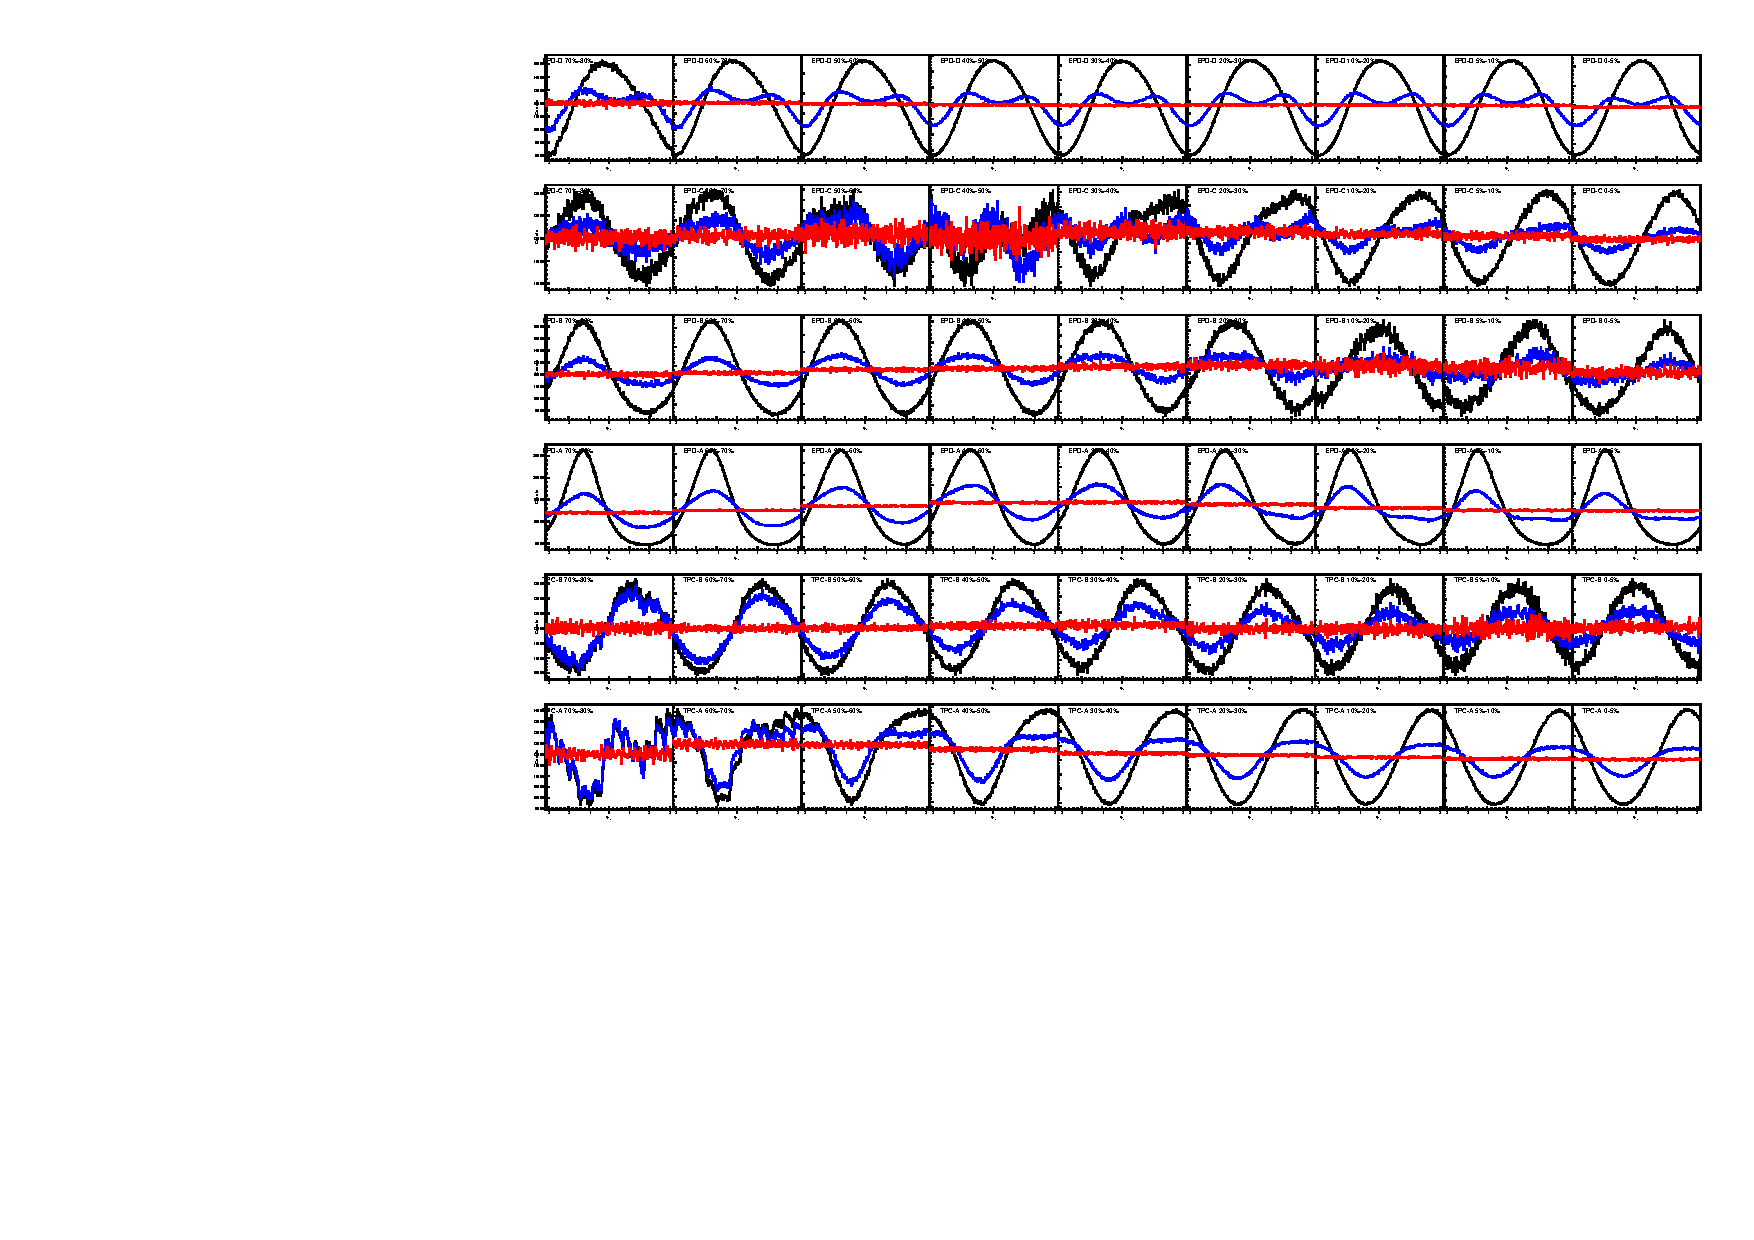
\includegraphics[scale=0.6]{chapter2/fig/epd_tpc_psi1_dis.pdf}
\caption{ TPC and EPD sub-event $\Psi_{1}$ distribution in different centrality, the black line is without raw $\Psi_{1}$ distribution, the blue line is with re-centering calibration, the red line is with re-centering and shift calibration}
\label{fig:epd_tpc_psi1}
\end{figure}

\begin{figure}[ht]
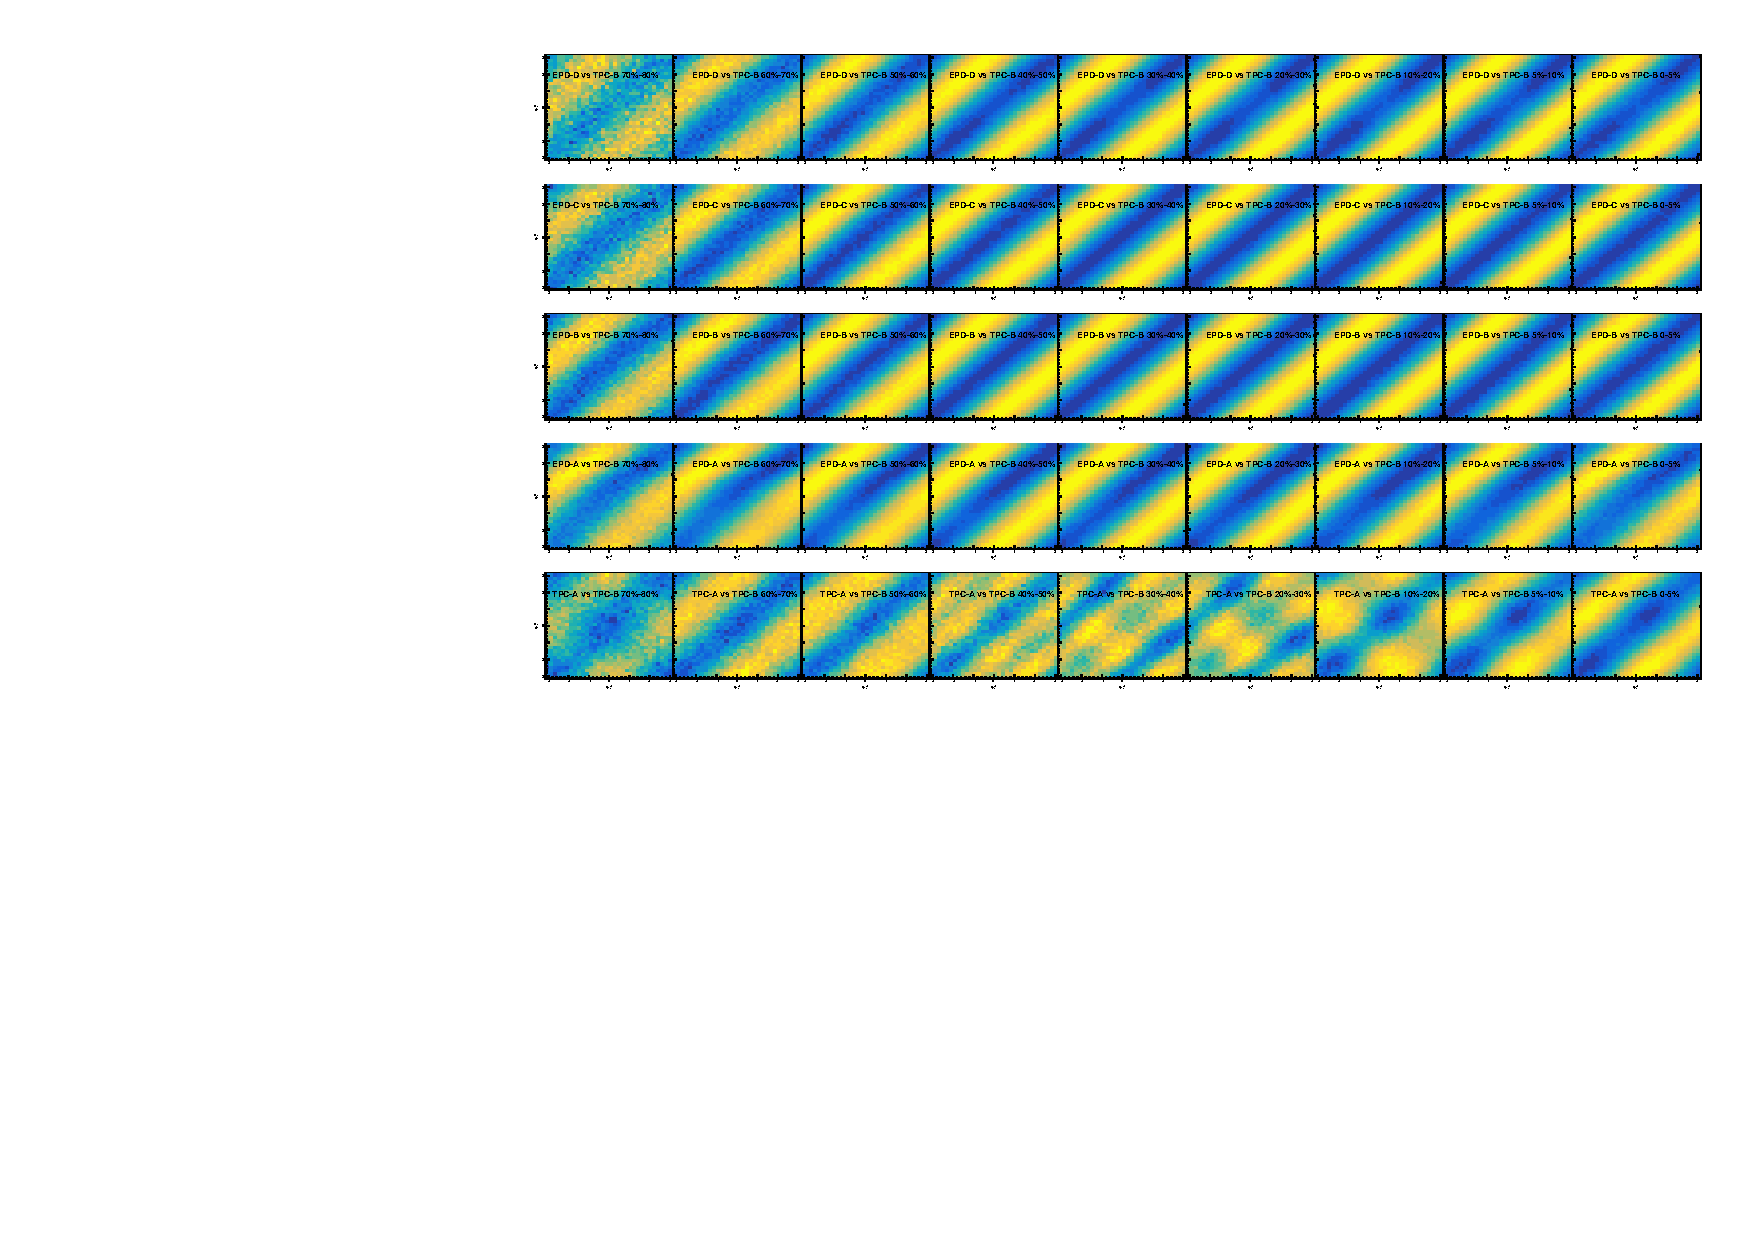
\includegraphics[scale=0.6]{chapter2/fig/epd_tpc_psi1_cor.pdf}
\caption{TPC and EPD sub-event event plane angle ($\Psi_{1}$) correlation}
\label{fig:epd_tpc_psi1_cor} 
\end{figure}


\newpage

\subsection{Event Plane Resolution}
Since the azimuthal angle of reaction plane is unknown, we use the event plane angle to estimate the reaction plane angle. Once we have the event plane angle ($\Psi_{1}$), then we can calculate the observed azimuthal anisotropy parameter ($v_{1}$, $v_{2}$). But the event plane deviates from the reaction plane, we need to correct the observed azimuthal anisotropy parameter ($v_{1}$, $v_{2}$) by event plane resolution. 
\begin{equation}
	v_{n} = \frac{v_{n}^{obs}}{R_{n}}
	=\frac{v_{n}^{obs}}{\left< cos[km(\Psi_{m}-\Psi_{r})] \right>}
	\label{equ:vn_cal}
\end{equation}
Where the $R_{n}$ is resolution, $v_{n}$ is the $n^{th}$ harmonic azimuthal anisotropy parameter, and $\Psi_{m}$ is the $m^{th}$ harmonic order event plane, k is integer number n $=$ k$*$m, $\Psi_{r}$ is reaction plane angle. The angle brackets denotes an average over all particles in all events. The event plane resolution can be expressed as:
\begin{equation}
	\left< cos[km(\Psi_{m}-\Psi_{r})] \right>=
	\frac{\sqrt{\pi}}{2\sqrt{2}}\chi_{m}exp(-\chi_{m}^{2}/4) \times
	[I_{(k-1)/2}(\chi_{m}^{2}/4)+I_{(k+1)/2}(\chi_{m}^{2})/4]
\end{equation}
Where $\chi_{m}$ $\equiv$ $v_{m}$$/$$\sigma$ and $I_{\nu}$ is the modified Bessel function of the order $\nu$. The resolution function is plotted in the figure \ref{fig:res_vs_nu}, the resolution is decreasing with k increases. Note that, numerically, when m = 1, the first order event plane angle can be used to calculate all $v_{n}$ term. In this analysis, we will use the first order event plane angle ($\Psi_{1}$) to calculate $v_{1}$ and $v_{2}$. Another reason is that, the magnitude of $n^{th}$ harmonic resolution is proportional to multiplicity and flow signal, the $v_{2}$ is decreasing with energy decreases. The second order event plane resolution is quite small at 3 GeV, which will induce large error for the $v_{2}$ results. While the $v_{1}$ is increasing with energy decreases. The error of $v_{2}$ calculated from $\Psi_{1}$ is 5 times smaller than that from $\Psi_{2}$. It will be discussed in the result part.

\begin{figure}[hb]
\centering
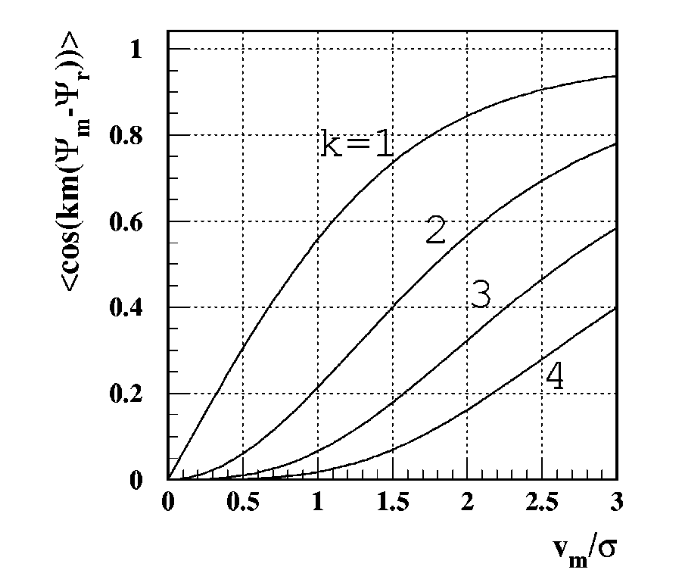
\includegraphics[scale=0.6]{chapter2/fig/resolution_vs_nu.png}
\caption{The event plane resolution for the $n^{th}$ (n=km) harmonic of the particle distribution with respect to the $m^{th}$ harmonic plane, as a function of $v_{m}$$/$$\sigma$.}
\label{fig:res_vs_nu} 
\end{figure}

Since we will use $\Psi_{1}$ to calculate $v_{1}$ and $v_{2}$, then we substitute (m=1, k=1) and (m=1, k=2) into the resolution equation to calculate the resolution for $v_{1}$ and $v_{2}$. $v_{1}$ and $v_{2}$ can be calculated with resolution shown in the following.

\begin{equation}
	R_{1} = \left< cos(\Psi_{1}-\Psi_{r}) \right>
	=\frac{\sqrt{\pi}}{2\sqrt{2}}\chi_{1}exp(-\chi_{1}^{2}/4) \times
	[I_{0}(\chi_{1}^{2}/4)+I_{1}(\chi_{1}^{2})/4]
	\label{equ:R1_chi1}
\end{equation}
\begin{equation}
	R_{12} = \left< cos(2(\Psi_{1}-\Psi_{r})) \right>
	=\frac{\sqrt{\pi}}{2\sqrt{2}}\chi_{1}exp(-\chi_{1}^{2}/4) \times
	[I_{1/2}(\chi_{1}^{2}/4)+I_{3/2}(\chi_{1}^{2})/4] 
	\label{equ:R12_chi1}
\end{equation}

\begin{equation}
	v_{1} =\frac{v_{1}^{obs}}{R_{1}} = 
	\frac{\left< cos(\phi-\Psi_{1}) \right>}{\left< cos(\Psi_{1}-\Psi_{r}) \right>}
\end{equation}
\begin{equation}
	v_{2} =\frac{v_{2}^{obs}}{R_{12}} = 
	\frac{\left< cos(2(\phi-\Psi_{1})) \right>}{\left< cos(2(\Psi_{1}-\Psi_{r})) \right>}
\end{equation}

Where the $R_{1}$ is the first order event plane resolution for $v_{1}$ and $R_{12}$ is second order event plane resolution estimated from first order event plane for $v_{2}$ calculation. In the equation \ref{equ:R1_chi1}, the $\chi_{1}$ is unknown. But we can first using three sub-event method to calculate the left hand first order event plane resolution ($R_{1}$), then we can determine the $\chi_{1}$, thus we substitute $\chi_{1}$ into equation \ref{equ:R12_chi1} to get the second order event plane resolution estimated from first order event plane for $v_{2}$ calculation ($R_{12}$). 

In the previous BES-I collider mode analysis, the resolution is determined from two sub-event method, which is required the multiplicity and flow signal of sub-events are same. This can be done by dividing the two sub-event from negative and positive $\eta$ range. But, if the sub-events are not "equal", or if we have only correlations between particles in different windows, and the resolution in each window can be different, then one needs at least three sub-events to determine the event plane resolution in each of them. In this case, the resolution in the first window is determined as:
\begin{equation}
	\left< cos(\Psi_{1}^{a}-\Psi_{r}) \right> = 
	\sqrt{\frac{\left< cos(\Psi_{1}^{a}-\Psi_{1}^{b}) \right>\left< cos(\Psi_{1}^{a}-\Psi_{1}^{c}) \right>}
	{\left< cos(\Psi_{1}^{b}-\Psi_{1}^{c}) \right>}}
\end{equation}
It's similar way to determine the other sub-event resolution. In this analysis, we divide the EPD to 4 sub-event groups, and we also combine the first two and last two group into one group, thus we have 6 sub-event groups and their resolution. as you can see in the figure \ref{fig:epd_1stres}, the first order event plane resolution as a function of centrality, different color and symbol means the same interest event plane resolution from different reference event plane. These difference will estimated into systematic uncertainties. From EPD-A to EPD-D, the resolution is decreasing with pseudorapidity decreases. This can be explained from that the $v_{1}$ signal is decreasing with pseudorapidity decreases.


\begin{figure}[ht]
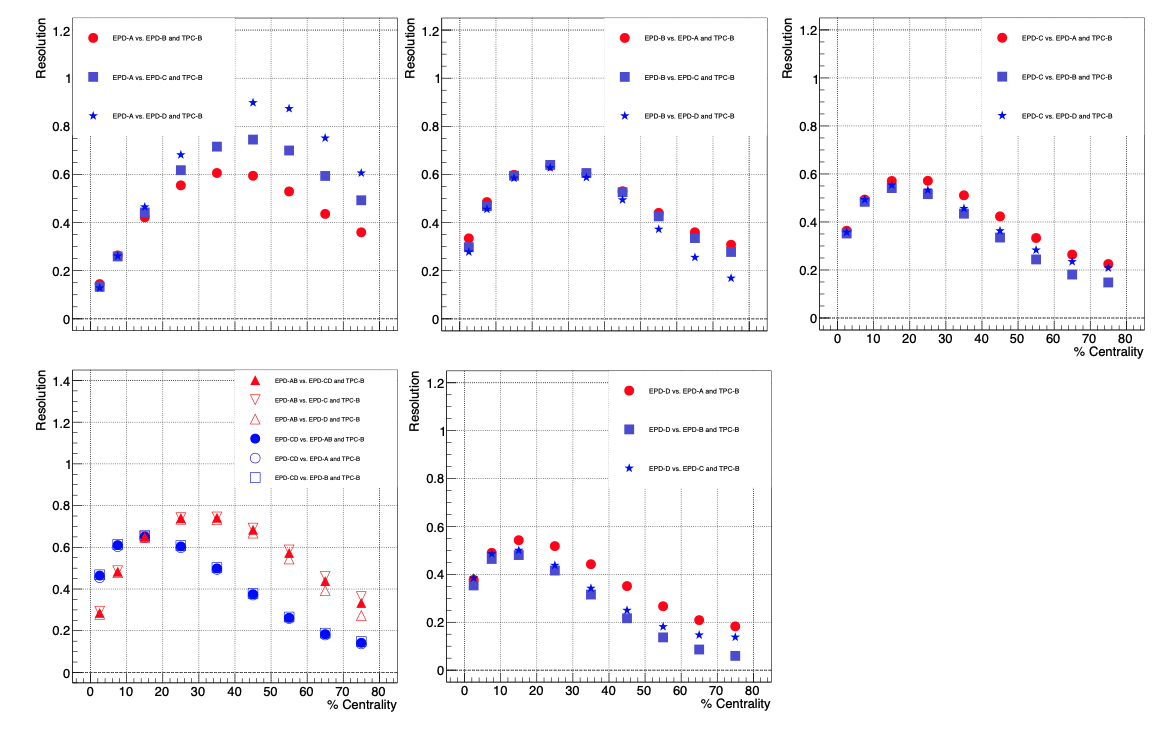
\includegraphics[scale=0.4]{chapter2/fig/epd_1stresolution.png}
\caption{ EPD First order event plane resolution as a function of centrality for different sub-event groups. Different symbol means the same interest event plane resolution using different reference event plane.}
\label{fig:epd_1stres}
\end{figure}



\subsection{$\pi$, $K$, $p$ Particle Identification}
\subsubsection{PID from TPC and TOF}
In this analysis, we use TPC and TOF detectors to identify particles (pion, kaon, and proton). Figure \ref{fig:dedx_mass2_3gev}, the left side, shows the TPC energy loss $dE/dx$ as a function of rigidity ($p/q$) with quality cuts. The curves for different color indicate the Bichsel expectation values for corresponding particles. As we can see, the TPC can identify particles at low momentum as illustrated by the color bands. At high momentum region, we need to identify particles together with TOF information. Figure \ref{fig:dedx_mass2_3gev}, the right side, shows the measured mass square as a function of rigidity ($p/q$) with track quality cuts. 

\begin{figure}[ht]
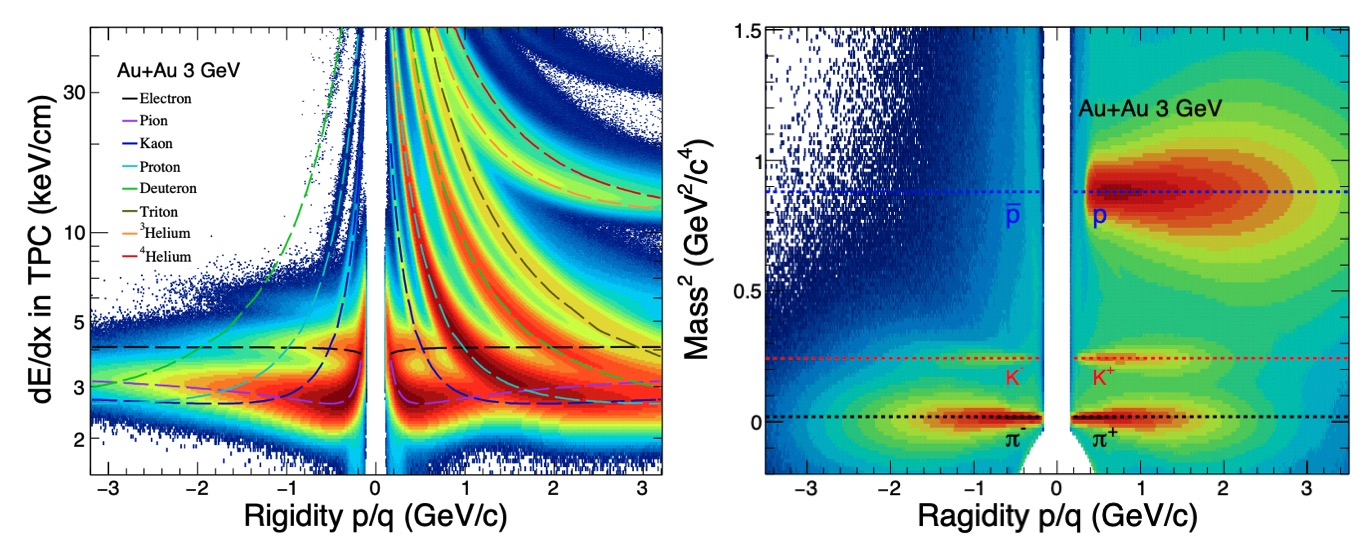
\includegraphics [scale=0.3]{chapter2/fig/dedx_3gev.png}
\caption{Left: Energy loss $dE/dx$ as a function of rigidity ($p/q$) for Au+Au collisions at $\sqrt{s_{NN}}$ = 3 GeV. The dash lines indicate the theoretical predicated values for different particles. Right: $Mass^{2}$ as a function of rigidity ($p/q$) for Au+Au collisions at $\sqrt{s_{NN}}$ = 3 GeV. The dash lines indicate the corresponding particles.}
\label{fig:dedx_mass2_3gev} 
\end{figure}

The $\left<dE/dx\right>$ distribution for a fixed particle type is not Gaussian. It has been shown that a better Gaussian variable, for a given particle type, is the $n\sigma_{particles}$, defined as:
\begin{equation}
	n\sigma_{particle} \propto ln \left[ \left< \frac{dE}{dX} \right>_{particle} / 
	\left< \frac{dE}{dX} \right>_{Bichsel} \right]
\end{equation}
where the particle type ($e^{\pm}, \pi^{\pm}, K^{\pm}, p, or  \bar{p}$) and $\left< \frac{dE}{dX} \right>_{Bichsel}$ is the corresponding Bichsel function. The most probable value of Bichsel function for the particle is 0.

The variable mass square ($m^{2}$) from TOF is given by:
\begin{equation} 
	m^{2} = p^{2} \left( \frac{c^{2}T^{2}}{L^{2}}-1 \right)
	\label{mass2_equ}
\end{equation}
where the p is the momentum, T is the time of travel by particle, L is the path length, and c is the speed of light.

\subsubsection{Acceptance of pion, kaon and proton}
In order to avoid fake tracks in the TPC and to improve the average momentum and energy loss resolution, the following track quality cuts in the table \ref{tab:tpc_cut_pid} were applied, then for the identification of pion, kaon and proton, we require TPC $n\sigma$ and TOF $mass^{2}$ cuts in the table \ref{tab:dedx_mass_cut_pid}. For pions and kaons, in addition of TPC $n_{\sigma}$ cut, we also apply TOF $m^{2}$ cut to improve their purity. For proton, since at 3GeV, the proton production will be dominated. So we only apply TPC $n_{\sigma}$ cut. Its purity is $>$ 95\% when the momentum $<$ 2 GeV, one can find the proton purity in different $p_{T}$ range in Fig. ~\cite{fig_proton_purity}. After these cuts, these particles acceptance plot ($\pi^{\pm}, K^{\pm}$, p ) can be found in the figure \ref{fig:pikp_acceptance_fig}, we also label the target location at $y = -1.045$, as we can see, the acceptance for all particles cover midrapidity region, so that we can make a fair comparison with STAR high energy results.
 
 \begin{table}[!ht]
\caption{\ TPC global tracks cuts for PID}
\label{tab:tpc_cut_pid}
\begin{tabular}{|c|c|}
\hline
nHitsFit$>$15 \\ \hline
nHitsFit/nHitsMax$>$0.52 \\ \hline
dca $<$ 3 (cm) \\ \hline
\end{tabular}
\end{table}


\begin{table}[ht]
\caption{\ dE/dX and $mass^{2}$ cut for PID}
\label{tab:dedx_mass_cut_pid}
\begin{tabular}{lclc|}
\hline
particle & cuts \\ \hline
pion  &  $|n\sigma_{\pi}|$ $<$ 3 and -0.1$<mass^{2}<$0.15 \\  \hline
kaon & $|n\sigma_{kaon}|$ $<$ 3 and 0.16$<mass^{2}<$0.36 \\ \hline
proton & $|n\sigma_{proton}|$ $<$ 2 when p$<$2.0GeV/c, $|n\sigma_{proton}|$ $<$ 2 and 0.6$<mass^{2}<$1.2 when p$>$2.0GeV/c  \\ \hline
\end{tabular}
\end{table}

\begin{figure}
    \centering
    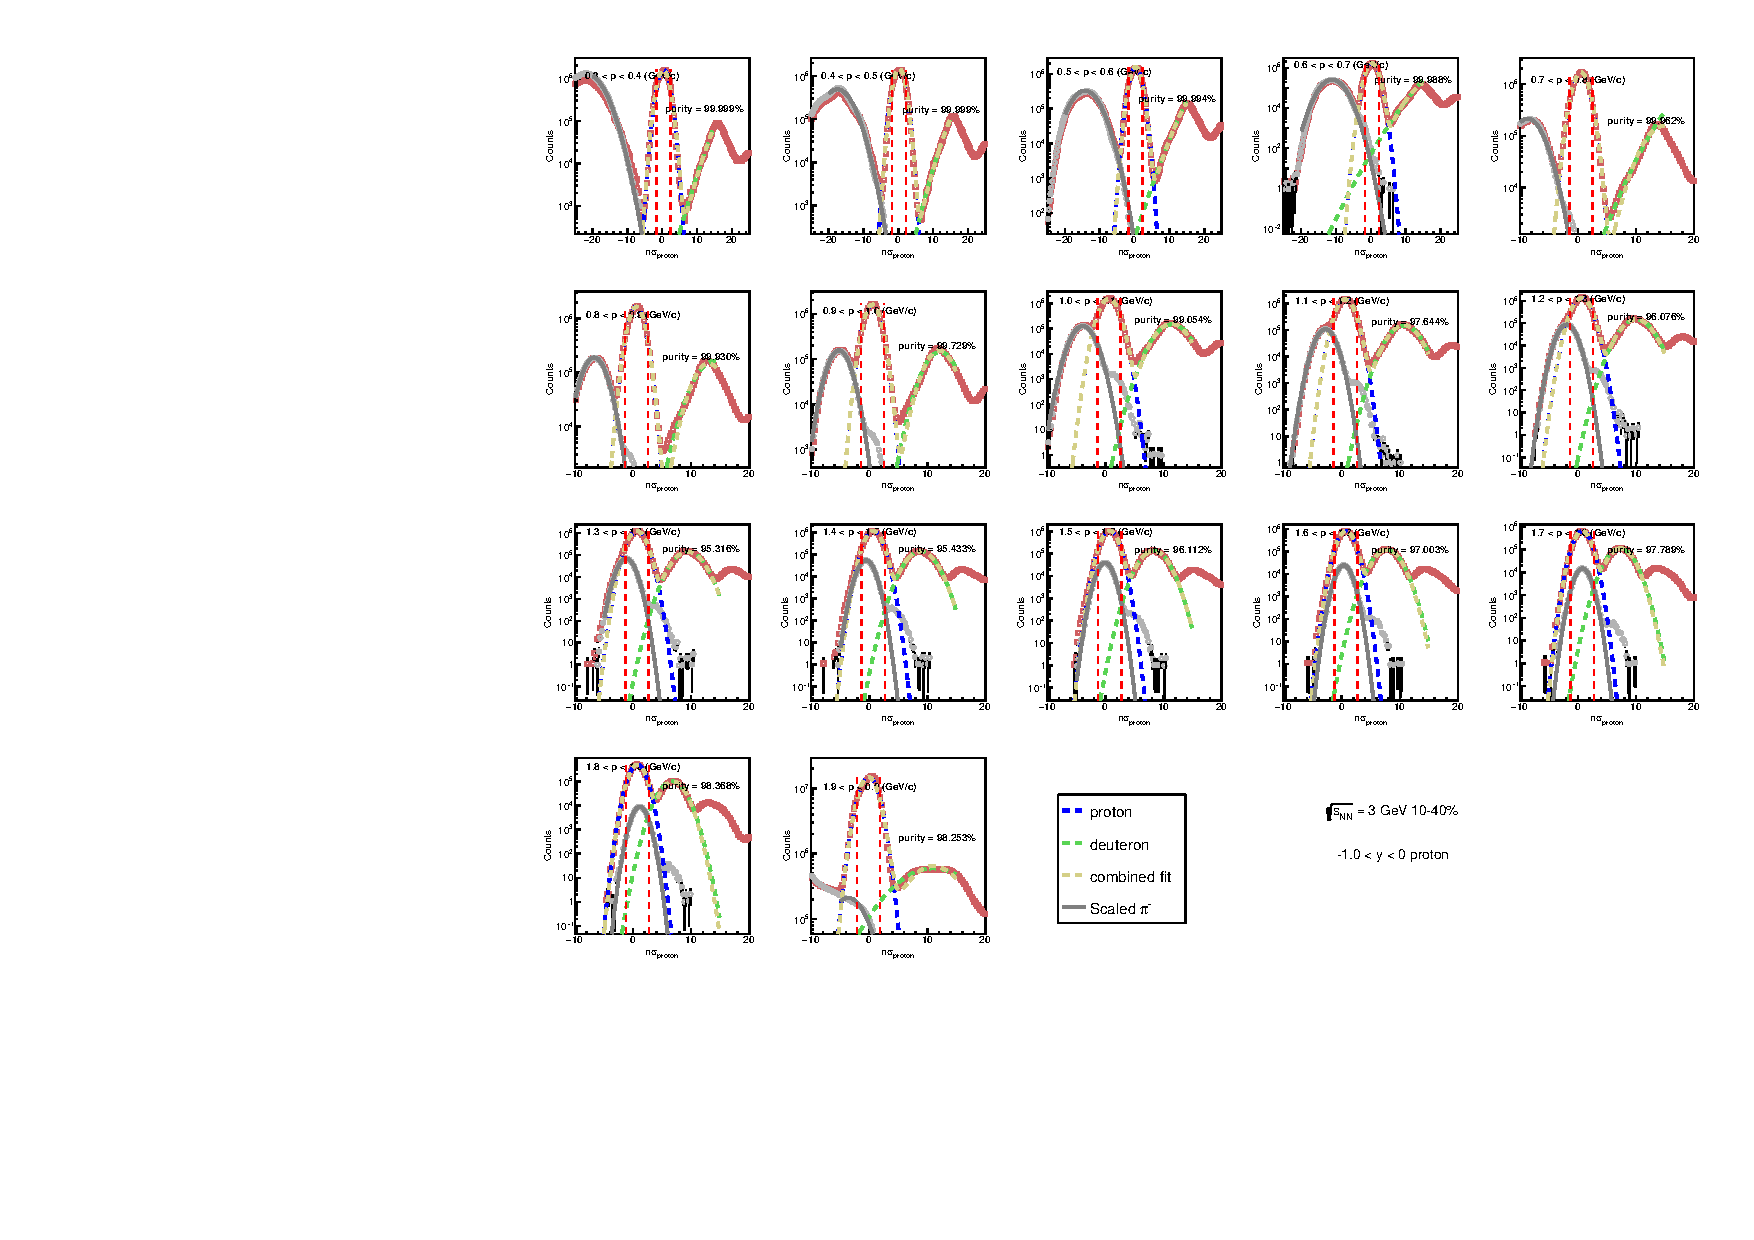
\includegraphics[scale=0.7]{FXT3gev/chapter2/fig/proton_purity.pdf}
    \caption{proton purity in different $p_T$ region (0.3-2.0 GeV)}
    \label{fig:proton_purity}
\end{figure}

\begin{figure}[ht]
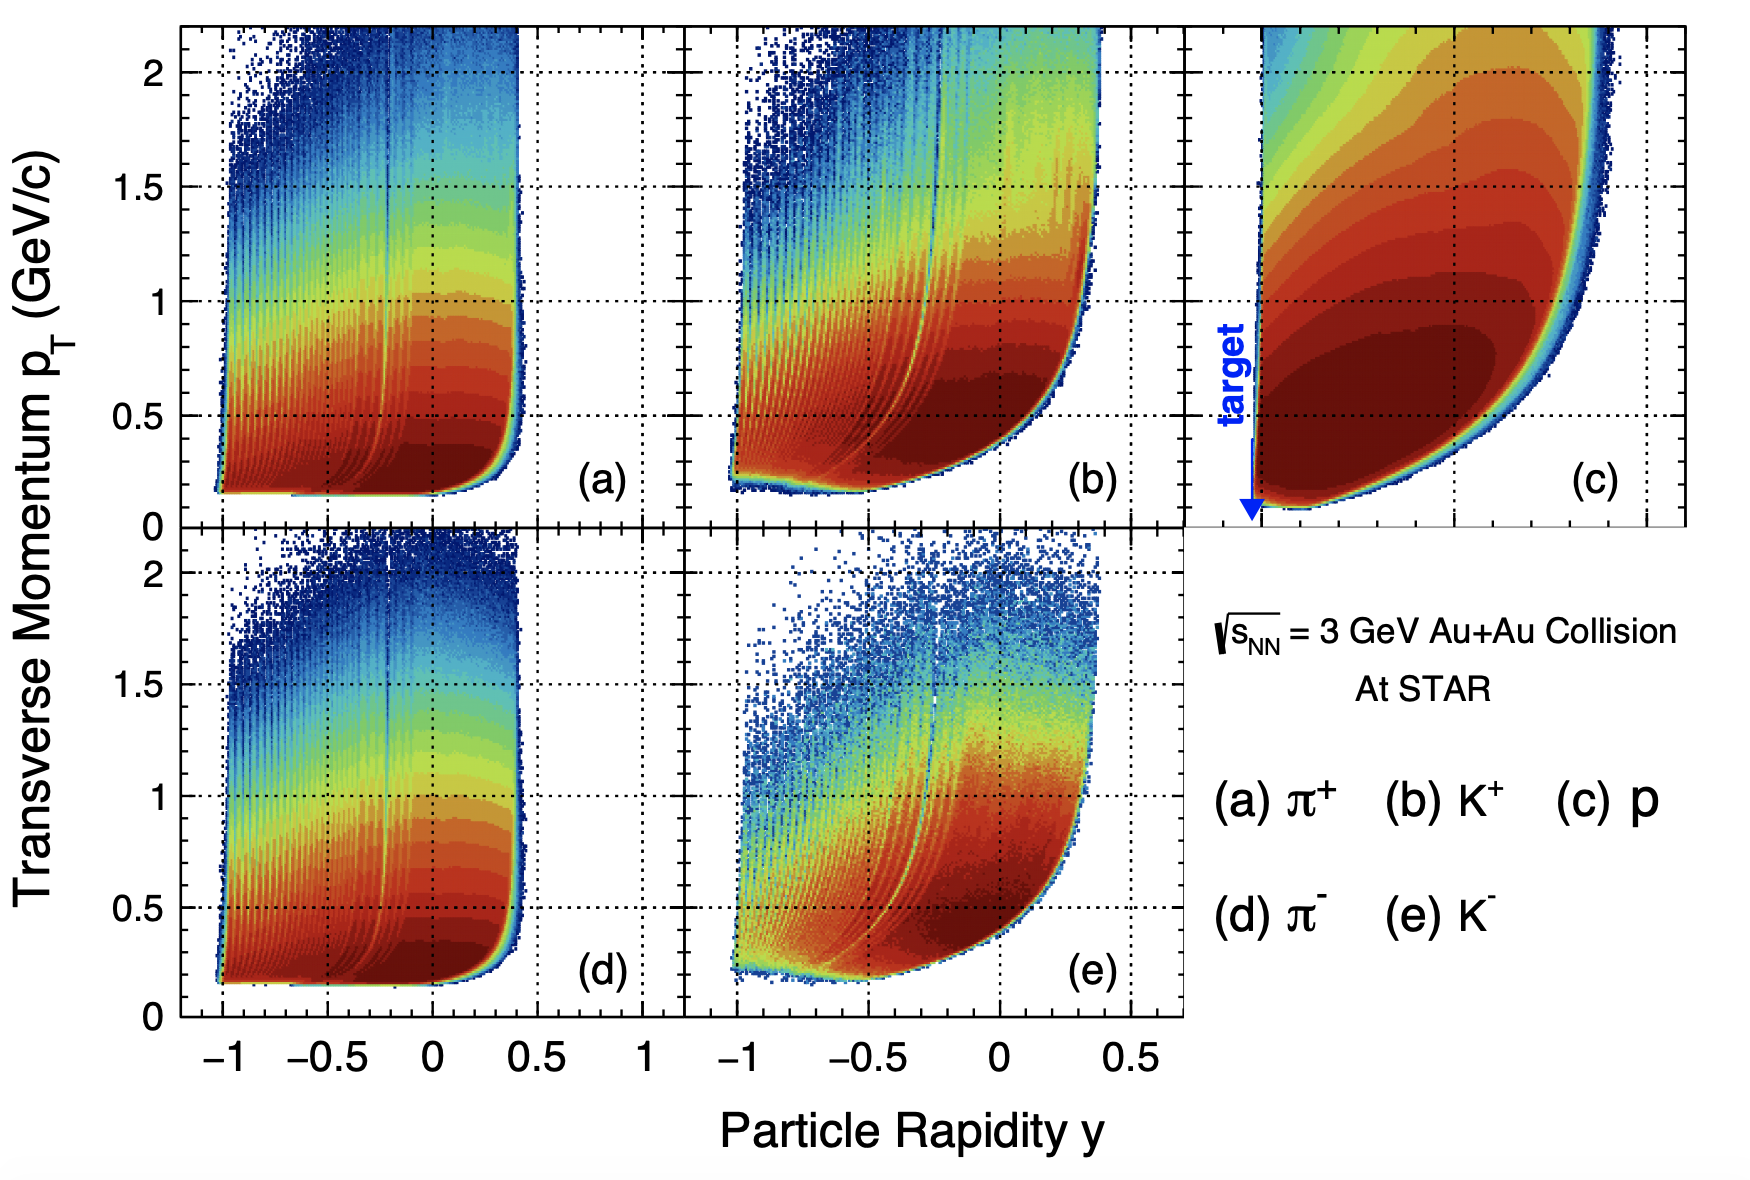
\includegraphics [scale=0.4]{chapter2/fig/pikp_acc_3gev.png}
\caption{ Rapidity(y) and transverse momentum($p_{T}$) acceptance of $\pi^{\pm}, K^{\pm}, proton$ using TPC and TOF in Au+Au collisions at $\sqrt{s_{NN}}$ = 3 GeV. The target is located at the y = -1.045. }
\label{fig:pikp_acceptance_fig}
\end{figure}

\clearpage
\newpage

\subsection{Efficiency Correction}

\subsubsection{TPC tracking efficiency}

The detector acceptance and the efficiency of reconstructing particle tracks are determined together by embedding Monte Carlo tracks simulated using the GEANT model \cite{Agostinelli:2002hh} of the STAR detector into real events at the raw data level. One important requirement is to have a match in the distributions of reconstructed embedded tracks and real data tracks for quantities reflecting track quality and used for track selection. The ratio of the distribution of reconstructed and original Monte Carlo tracks as a function of $p_{T}$ and rapidity gives the efficiency x Acceptance correction factor for the $p_{T}$ and rapidity interval studies. 
	
Figure \ref{fig:pikp_eff_tpc} shows the pion, kaon and proton TPC tracking efficiency as a function of $p_{T}$ and rapidity. In the FXT model collision, we do see efficiency alone the $p_{T}$ and rapidity direction. So, we plot the efficiency of particle species as a function of $p_{T}$ and rapidity. The track-by-track TPC tracking efficiency correction will be included in this analysis.

\begin{figure}
    \centering
    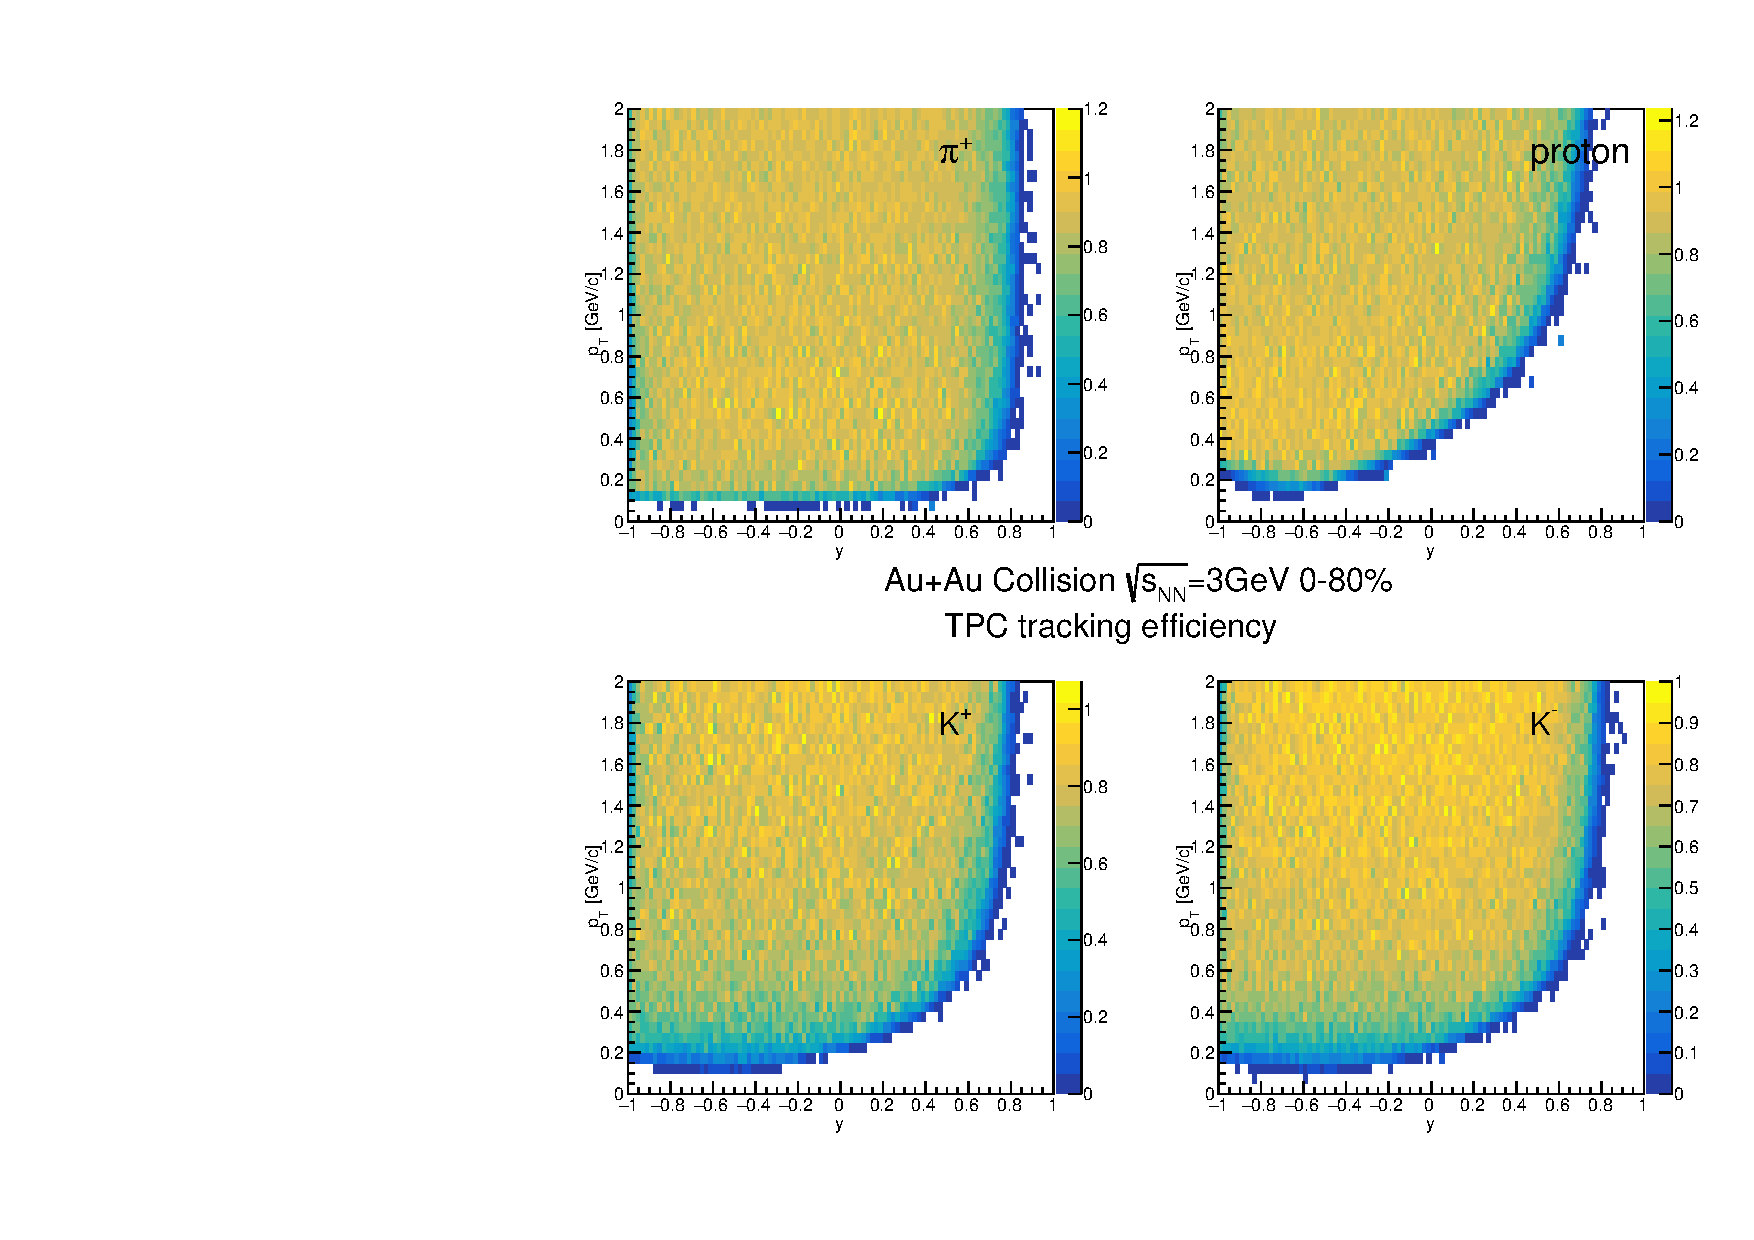
\includegraphics[scale=0.5]{FXT3gev/chapter2/fig/eff/pik_tpceff.pdf}
    \caption{pion, kaon, proton tracking efficiency as a function of $p_{T}$ and rapidity in 0-80\% for two-dimensional}
    \label{fig:pikp_eff_tpc}
\end{figure}
	
\subsubsection{TOF matching efficiency}

Since the TOF can give better particle identification than TPC at higher momentum region, however not all TPC tracks can travel into TOF and give a hit. So there is an extra correction called TOF matching efficiency correction used in our analysis. This is done with a data-driven technique. The TOF matching efficiency $\epsilon$ can be determined by number of TOF matched tracks divide by number of TPC tracks as shown in the formula \ref{equ:TOF_eff}. 
figure \ref{fig:pik_eff_tof} shows the two-dimensional efficiency as a function of $p_{T}$ and rapidity (y) in 0-80\% for pions and kaons. Since we give the additional $m^{2}$ cut for pions and kaons.
The track-by-track TPC tracking associated TOF matching efficiency correction will be applied into our analysis.

\begin{equation}
    \epsilon (p_{T}, y) = \frac{\text{Number of TOF Matched Tracks}}{\text{Number of TPC Tracks}}
    \label{equ:TOF_eff}
\end{equation}

\begin{figure}
    \centering
    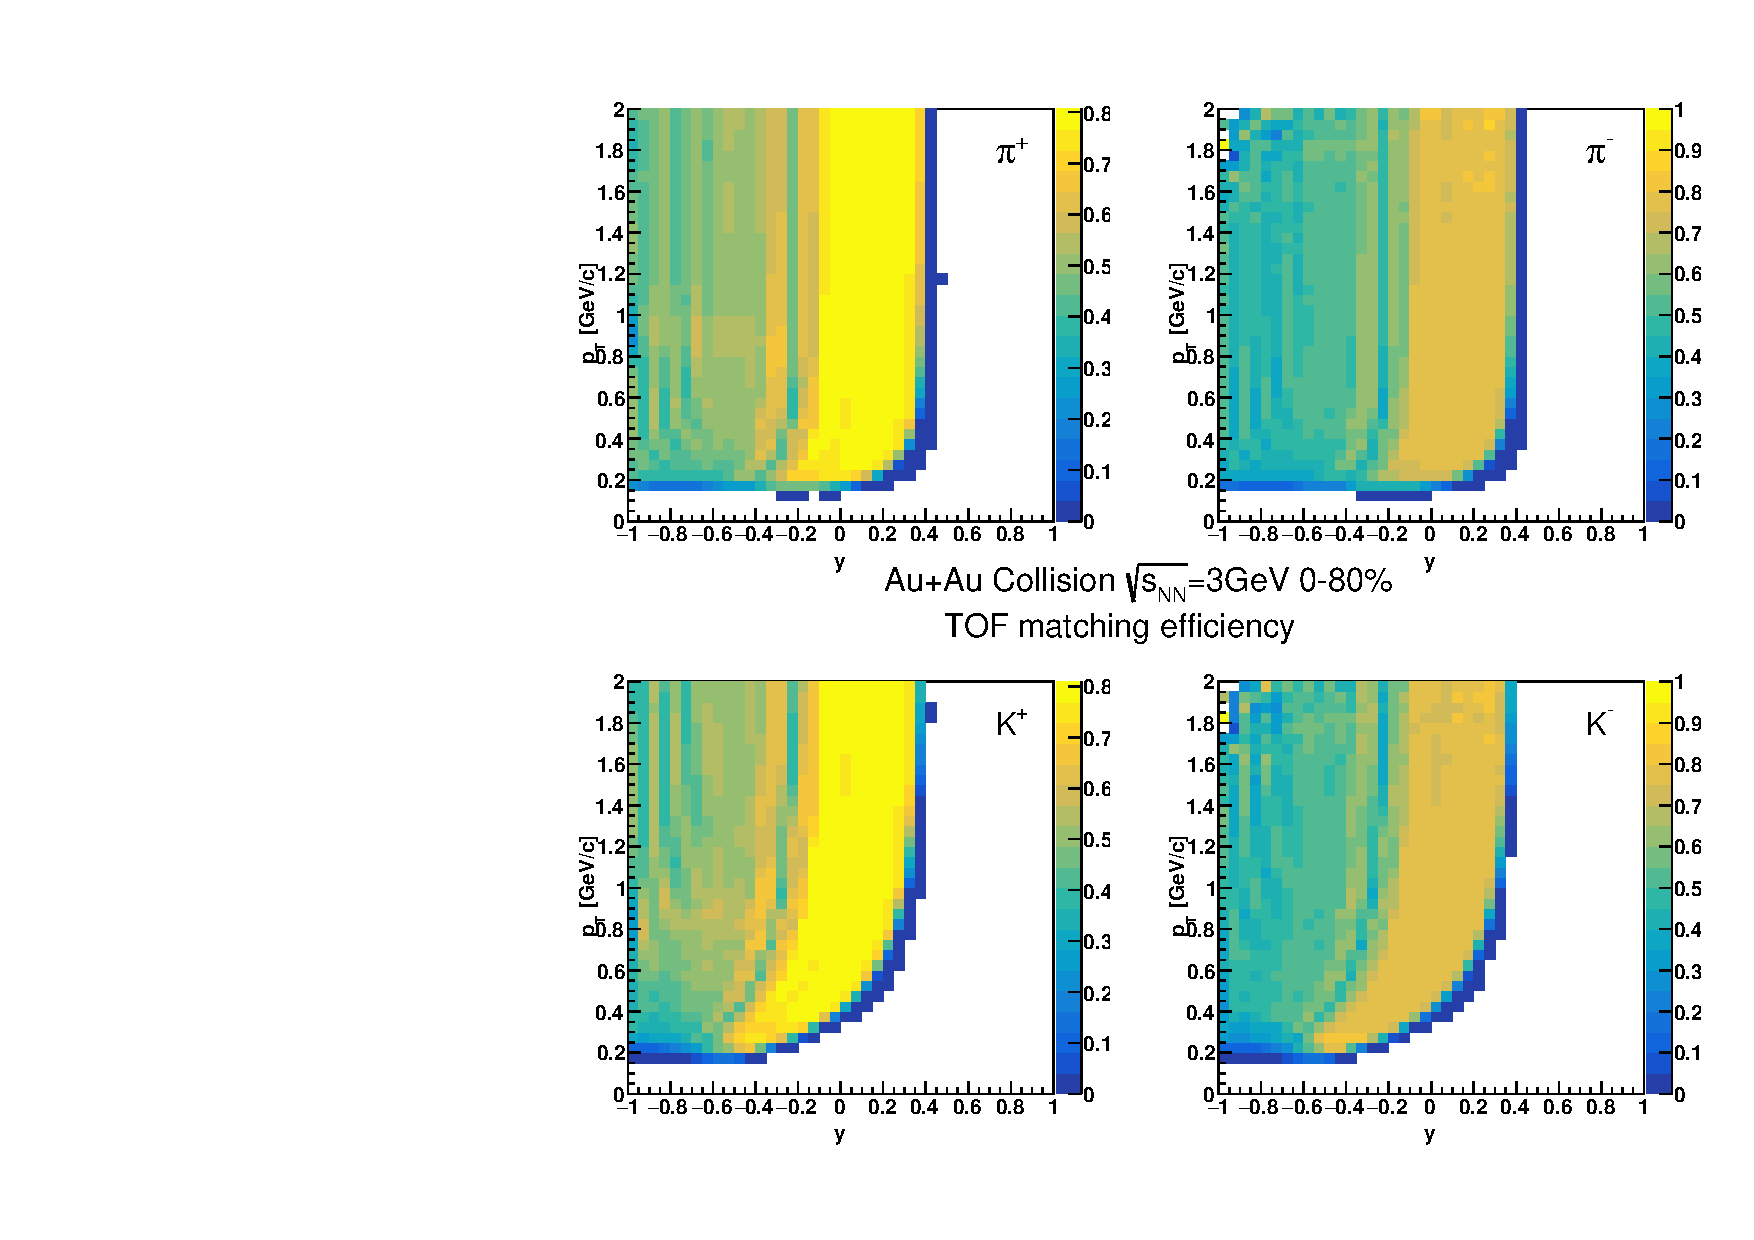
\includegraphics[scale=0.5]{FXT3gev/chapter2/fig/eff/pik_tofeff.pdf}
    \caption{pion, kaon TOF matching efficiency as a function of $p_{T}$ and rapidity in 0-80\% for two-dimensional}
    \label{fig:pik_eff_tof}
\end{figure}

%Analysis detail
\clearpage
\section{Results} 
In this section, we show the results of $v_{1}$ and $v_{2}$ for pions, kaons, and proton. The $p_{T}$ and rapidity dependence will be discussed and performed in three centrality classes 0-10\%, 10-40\% and 40-60\%. These results will be comparison to STAR BES-I results and the physics meaning will be discussed.

\subsection{$v_{1}$ results for $\pi, K, p$}
In this chapter, we will show the $v_{1}$ as a function of $p_{T}$ and rapidity(y) in fine centrality bins for $\pi^{\pm}, K^{\pm}$ and proton. In the $v_{1}$  vs. rapidity distribution, in order to quantify the strength of  $v_{1}$, we will fit the $v_{1}$ vs. y distribution with this equation \ref{fit_v1_formula}. As can see, pion's $v_{1}$ is positive in the central collision while is negative in the mid-central and peripheral collision.

\begin{equation} \label{fit_v1_formula}
	v_{1}(y) = F*y + C*y^{3} +b 
\end{equation}
Where parameter F is the $v_{1}$ slop $dv_{1}/dy$, parameter C is the fluctuation term and parameter b is the offset to origin point.

\subsubsection{pions $v_{1}$ as a function of $p_{T}$ and rapidity}
Figure \ref{pion_v1y_cent} shows $\pi^{+}, \pi^{-}$ $v_{1}$ as a function of y for different centrality bins from 0-5\% to 50-60\%,  the red line is fitting function \ref{fit_v1_formula}, the $p_{T}$ range is [0.2, 1.6] GeV/c, which is same with STAR BES-I results. We also write down the fitted results $v_{1}$ slope $dv_{1}/dy$. As we can see, the magnitude of pions' $v_{1}$ has centrality dependence, figure \ref{pion_dv1dy_cent} shows $\pi^{+}, \pi^{-}$ $dv_{1}/dy$ as a function of centrality, we can clear see that the $v_{1}$ sign change from central to peripheral collision. This can be explained by the shadowing effect from spectators, because at 3 GeV, the passage time is comparable or larger than medium expansion time. So, the spectators will shadow the expansion of mediums, which will cause negative $v_{1}$ value, and this effect larger with collisions from central collision to peripheral collision.

Since STAR's BES-I directed flow results focus on the intermediate centrality interval 10-40\%. In this analysis, we also have $v_{1}$ results in such centrality bins for these particle species, and, we will calculate the energy dependence for all particles' $v_{1}$. Figure \ref{pion_v1y_widecent} shows $\pi^{+}$ and $\pi^{-}$ $v_{1}$ as a function of y in 0-10\%, 10-40\% and 40-60\% bins. We can see in the 0-10\%, the pions' $v_{1}$ is positive, and the the pions' $v_{1}$ is negative in the 10-40\% and 40-60\% centralities, which can be explained by the spectator shadowing effect.

\begin{figure}[h]
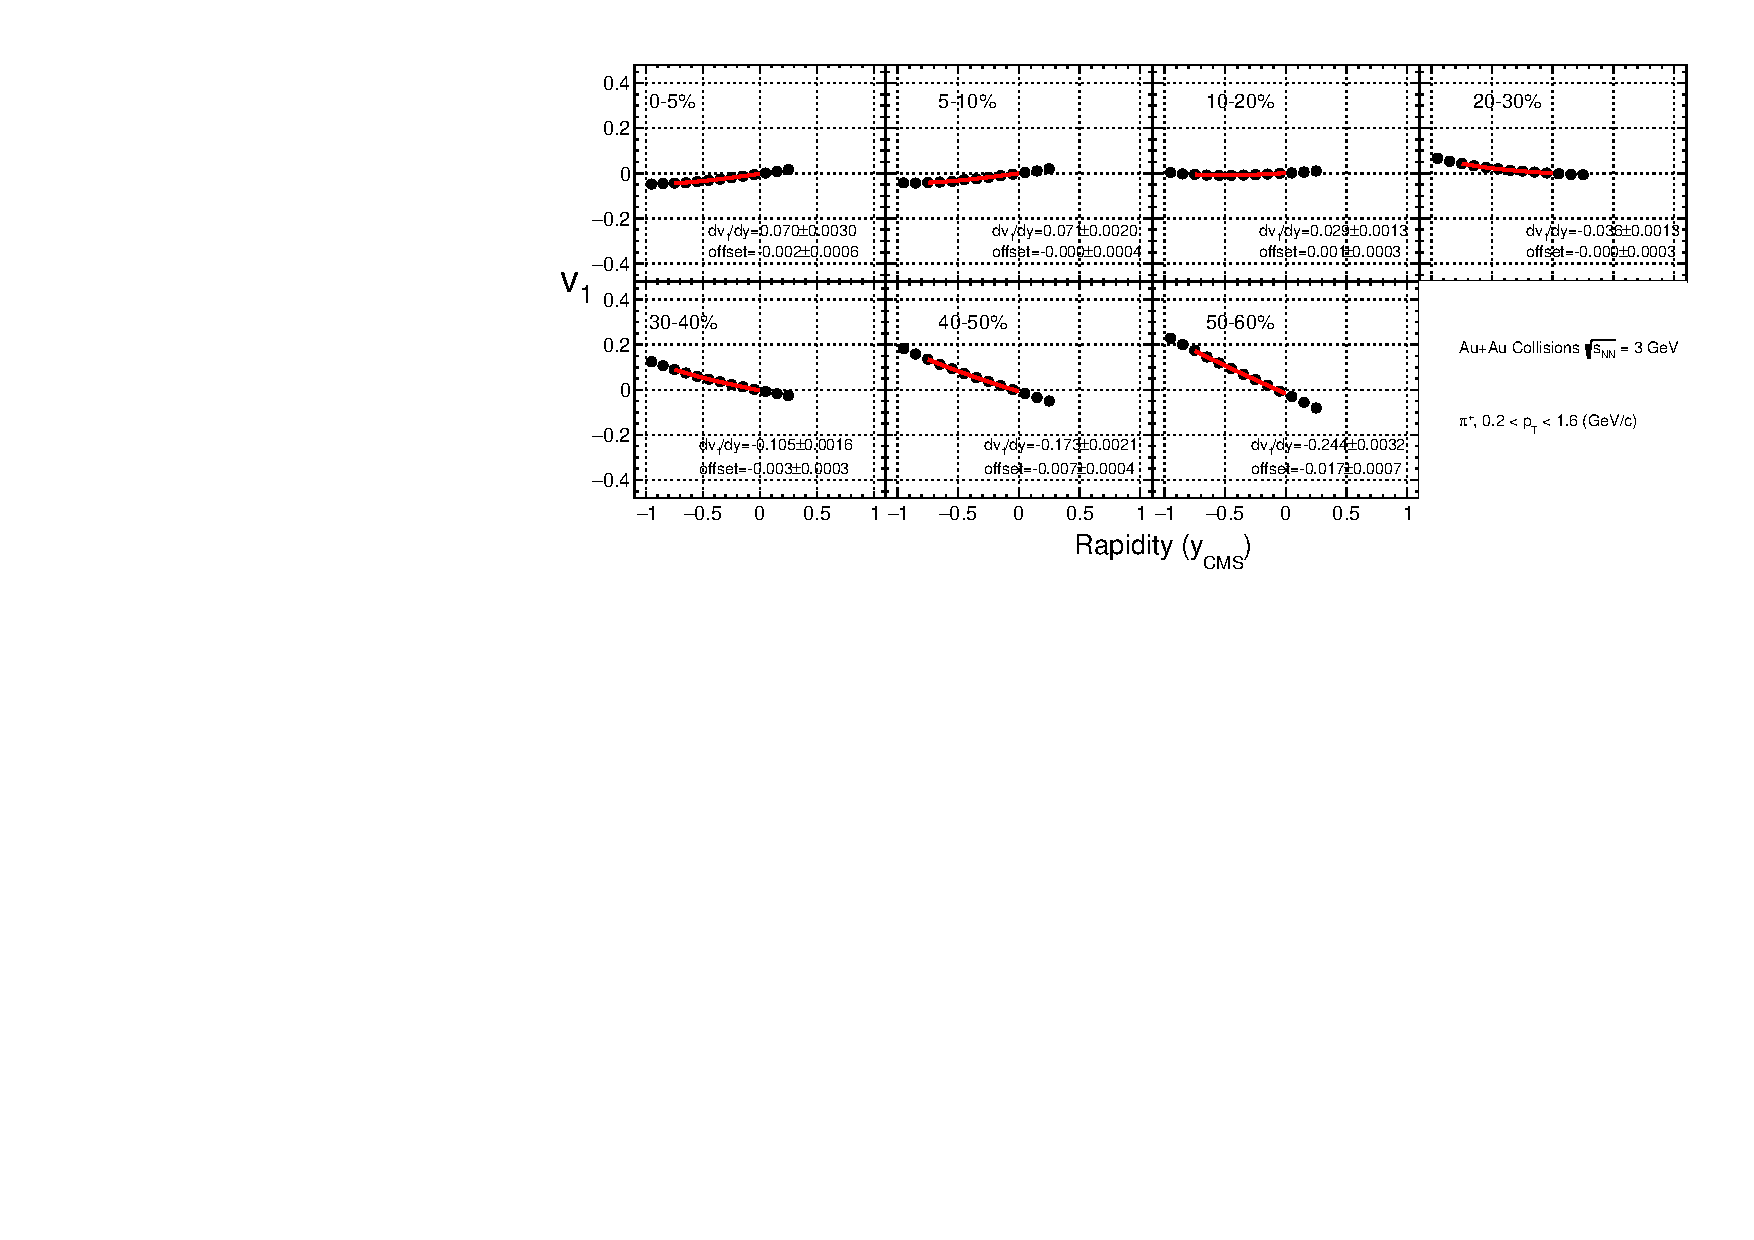
\includegraphics[scale=0.6]{chapter3/fig/v1ypikp/v1pionp_cent.pdf}
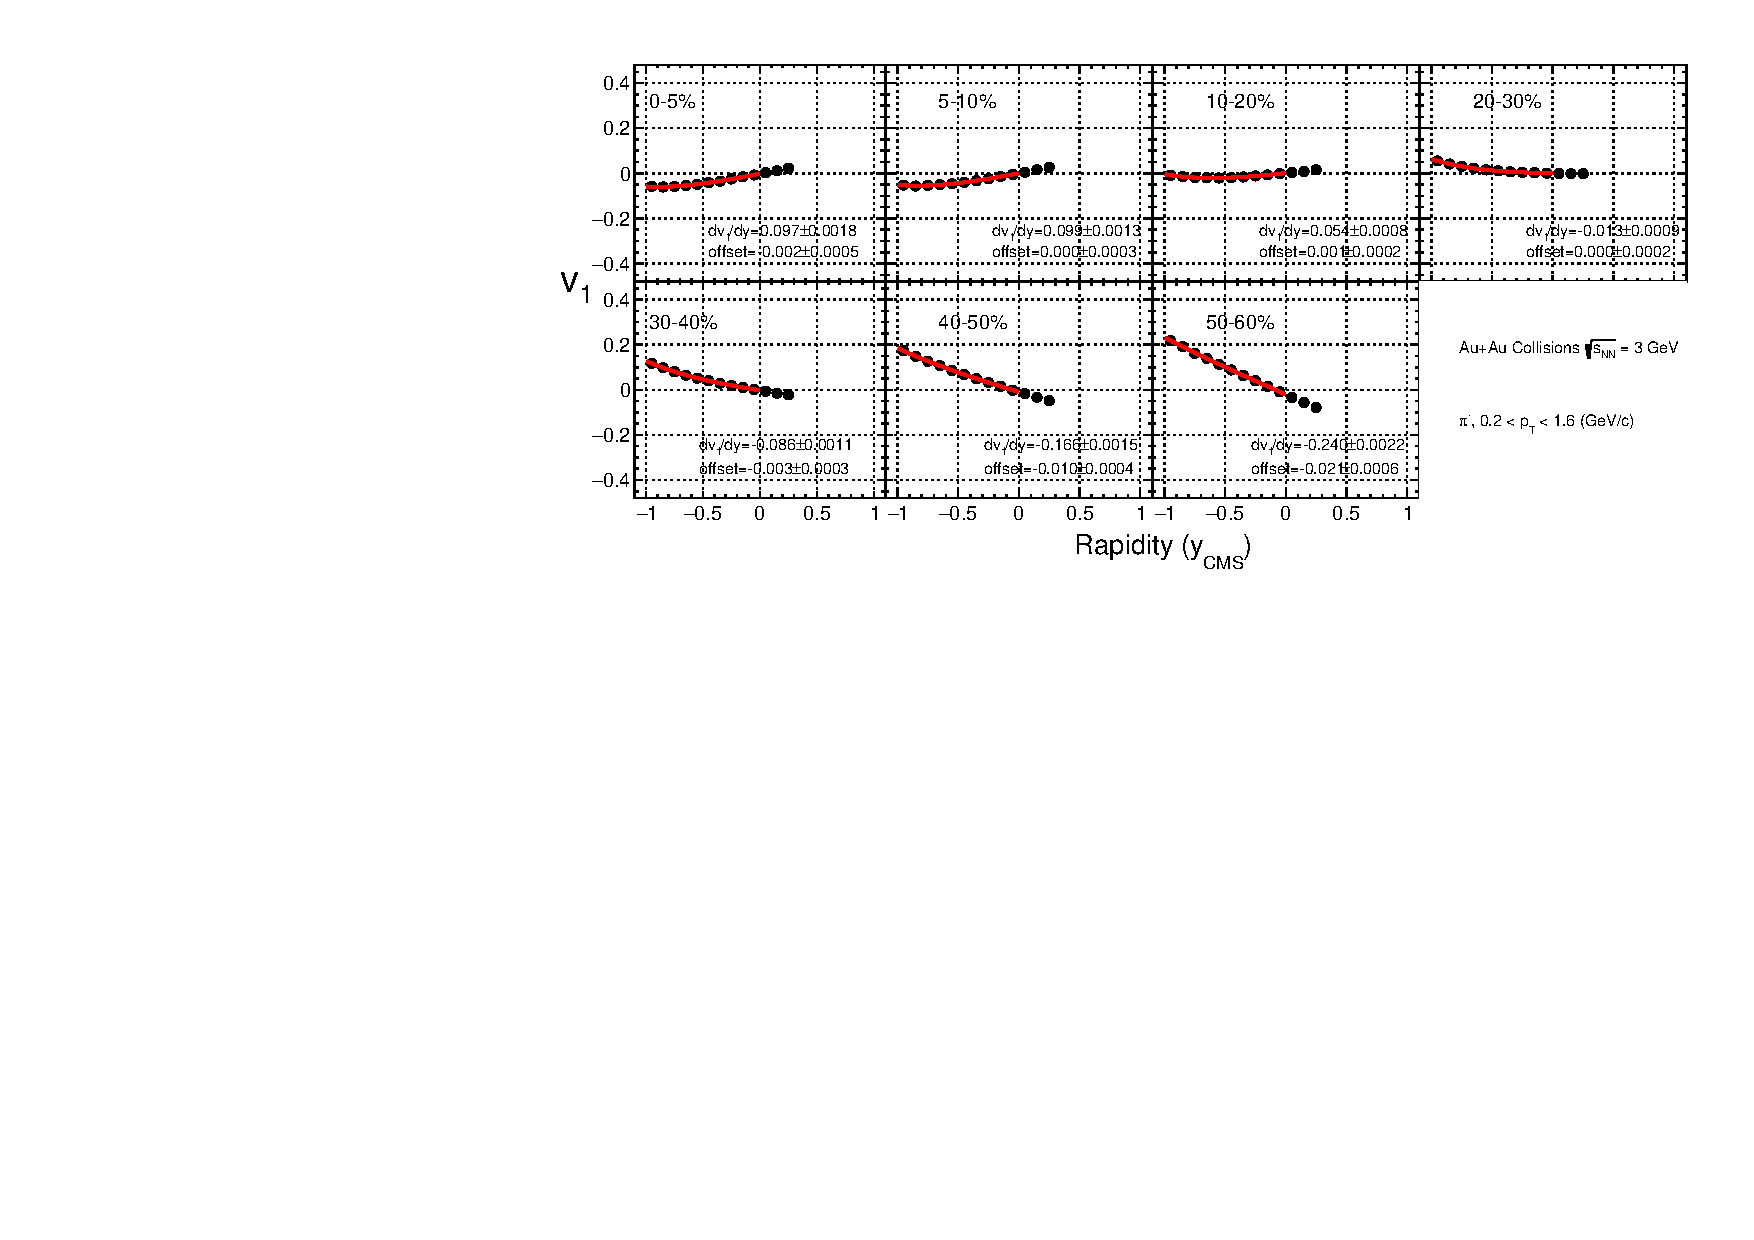
\includegraphics[scale=0.6]{chapter3/fig/v1ypikp/v1pionm_cent.pdf}
\caption{\label{pion_v1y_cent} $v_{1}$ as a function of rapidity(y) in different centrality bins for $\pi^{+}$ and $\pi^{-}$ in Au+Au collisions at $\sqrt{s_{NN}}$. The red line is fitting function.}
\end{figure}

\begin{figure}[h]
\centering
\subfigure{   
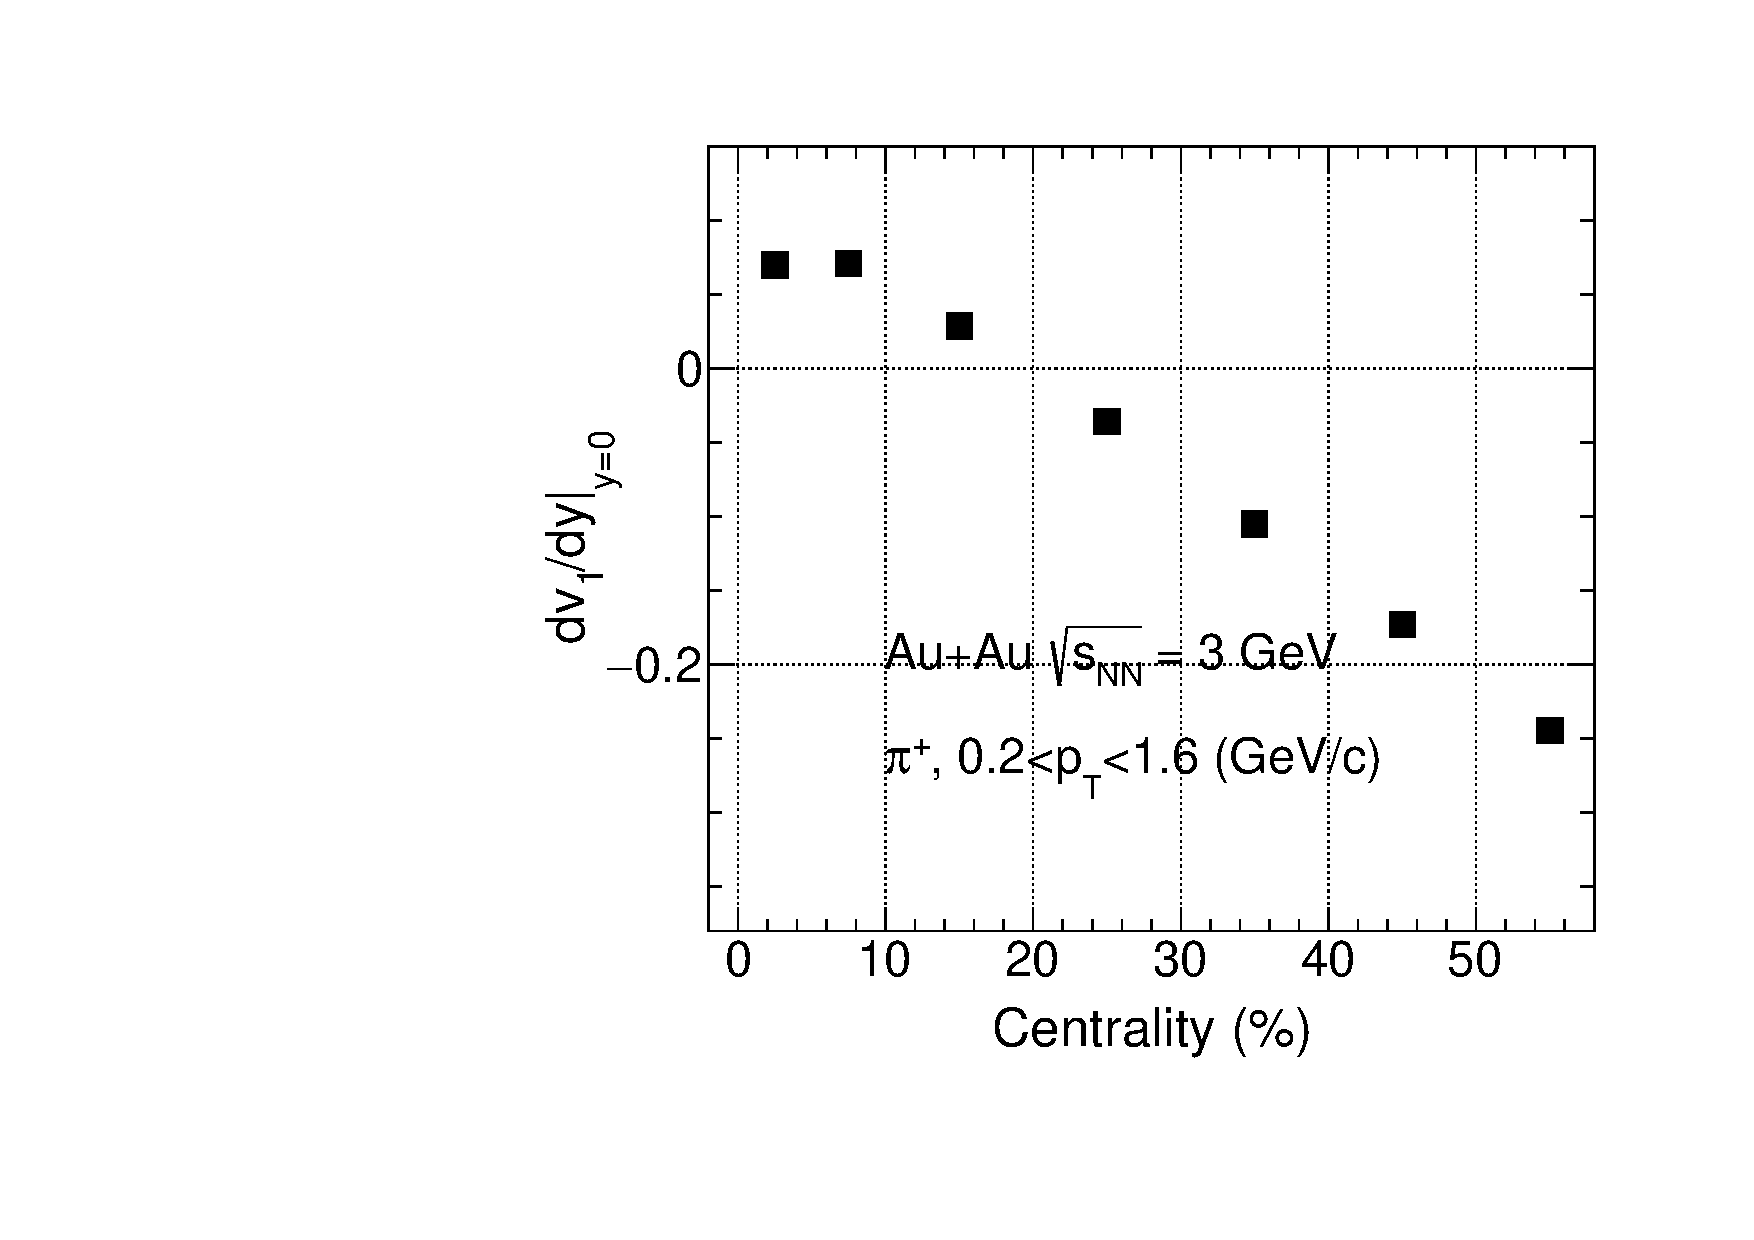
\includegraphics[width=0.45\textwidth]{chapter3/fig/v1ypikp/dv1dy_pionp.pdf}}
\subfigure{
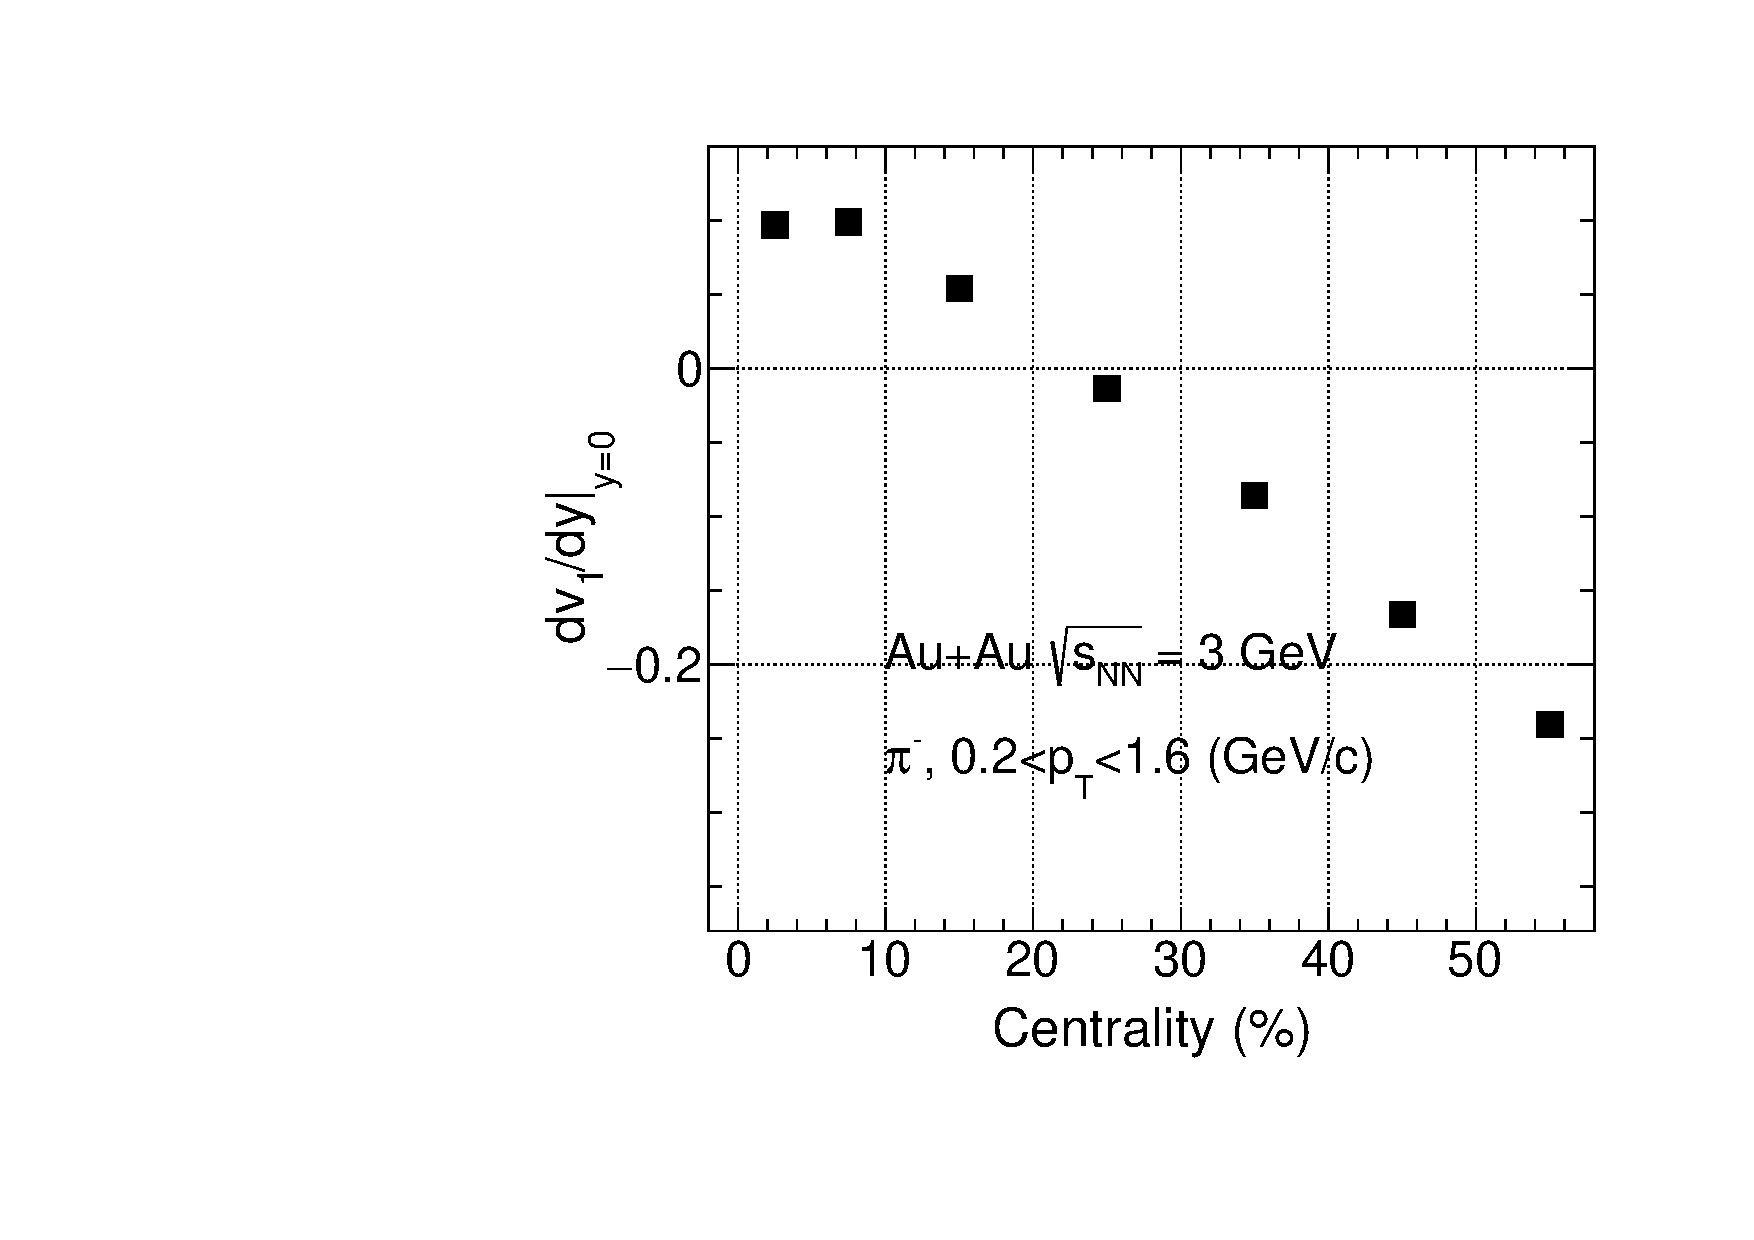
\includegraphics[width=0.45\textwidth]{chapter3/fig/v1ypikp/dv1dy_pionm.pdf}}
\caption{\label{pion_dv1dy_cent} pions' $v_{1}$ slope $dv_{1}/dy$ as a function of centrality, (left) $\pi^{+}$ (right) $\pi^{-}$ in Au+Au collisions $\sqrt{s_{NN}}$ = 3GeV.}
\end{figure}

\begin{figure}[h]
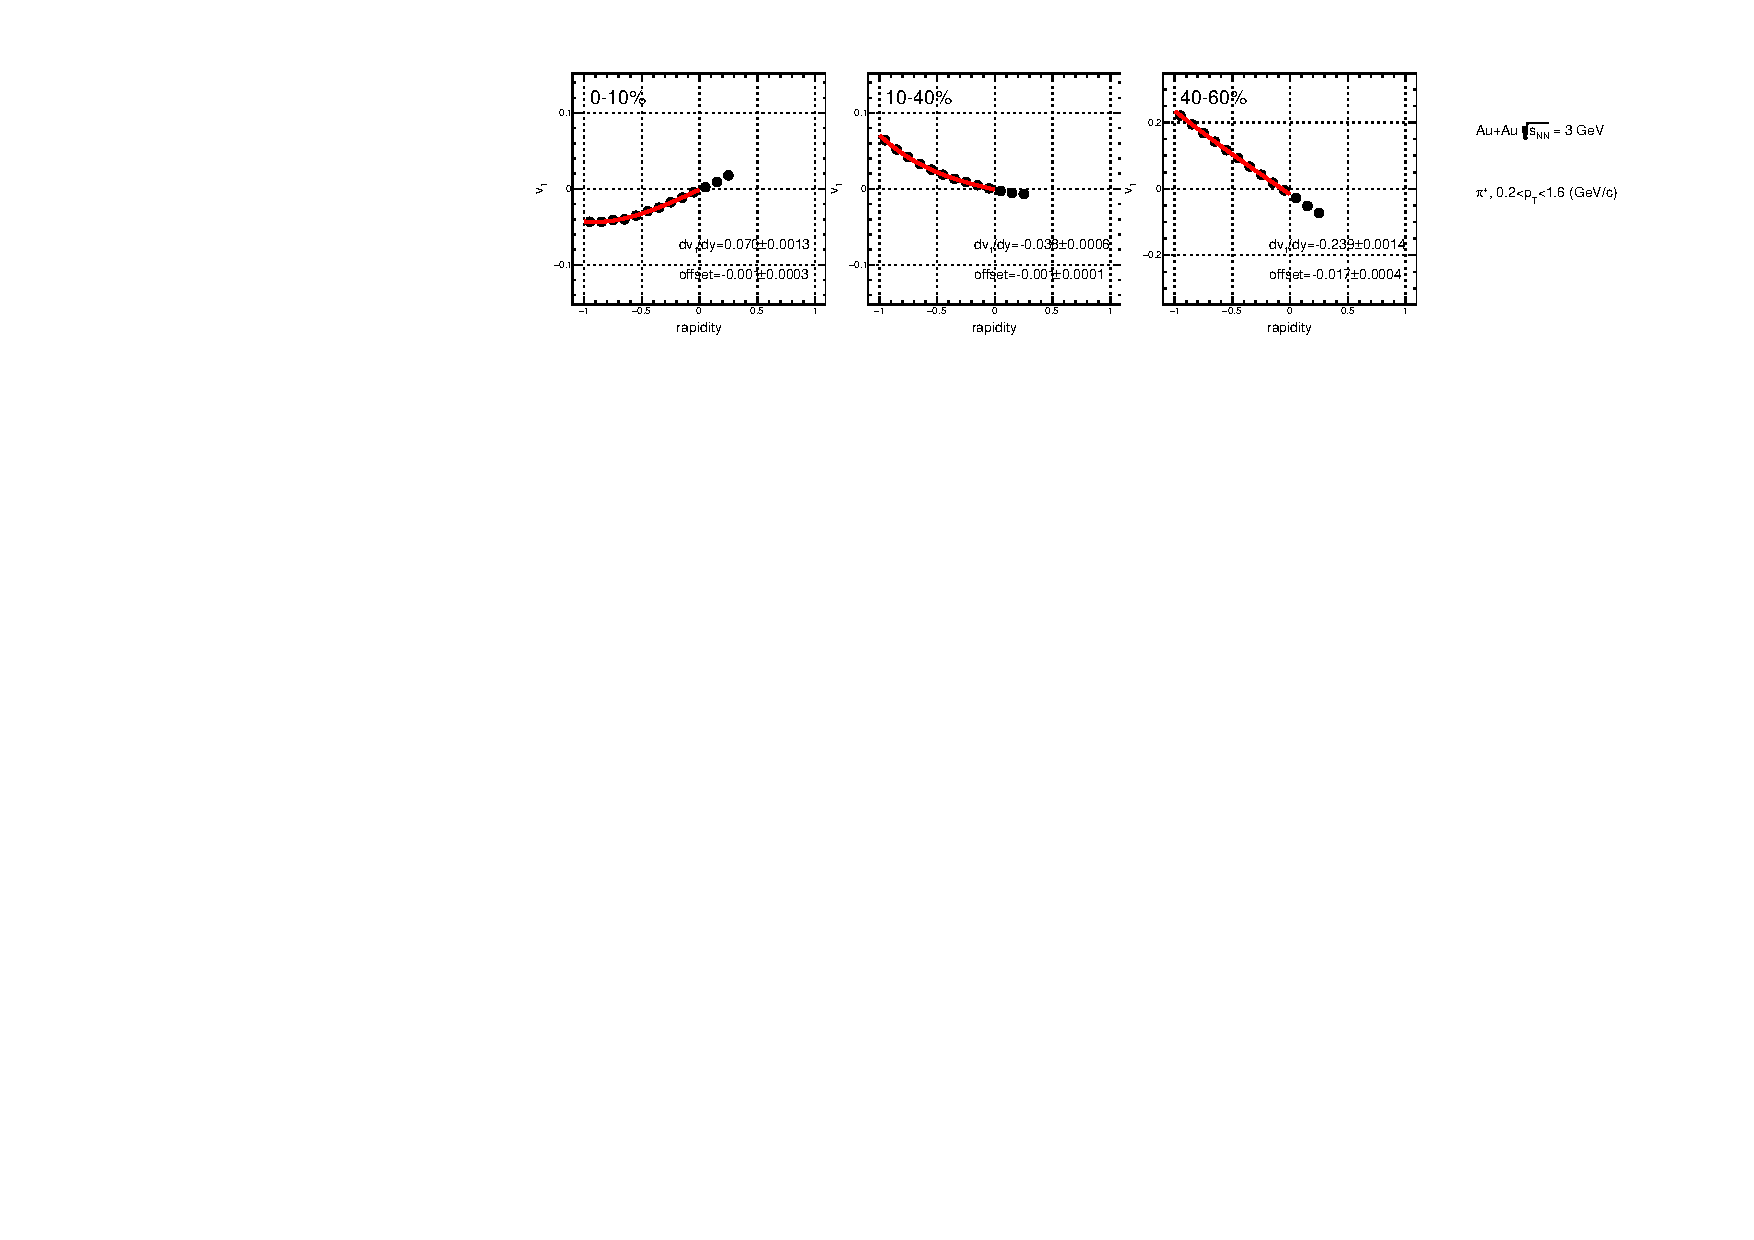
\includegraphics[scale=0.8]{chapter3/fig/v1ypikp/pionp_v1y_wide_cent.pdf}
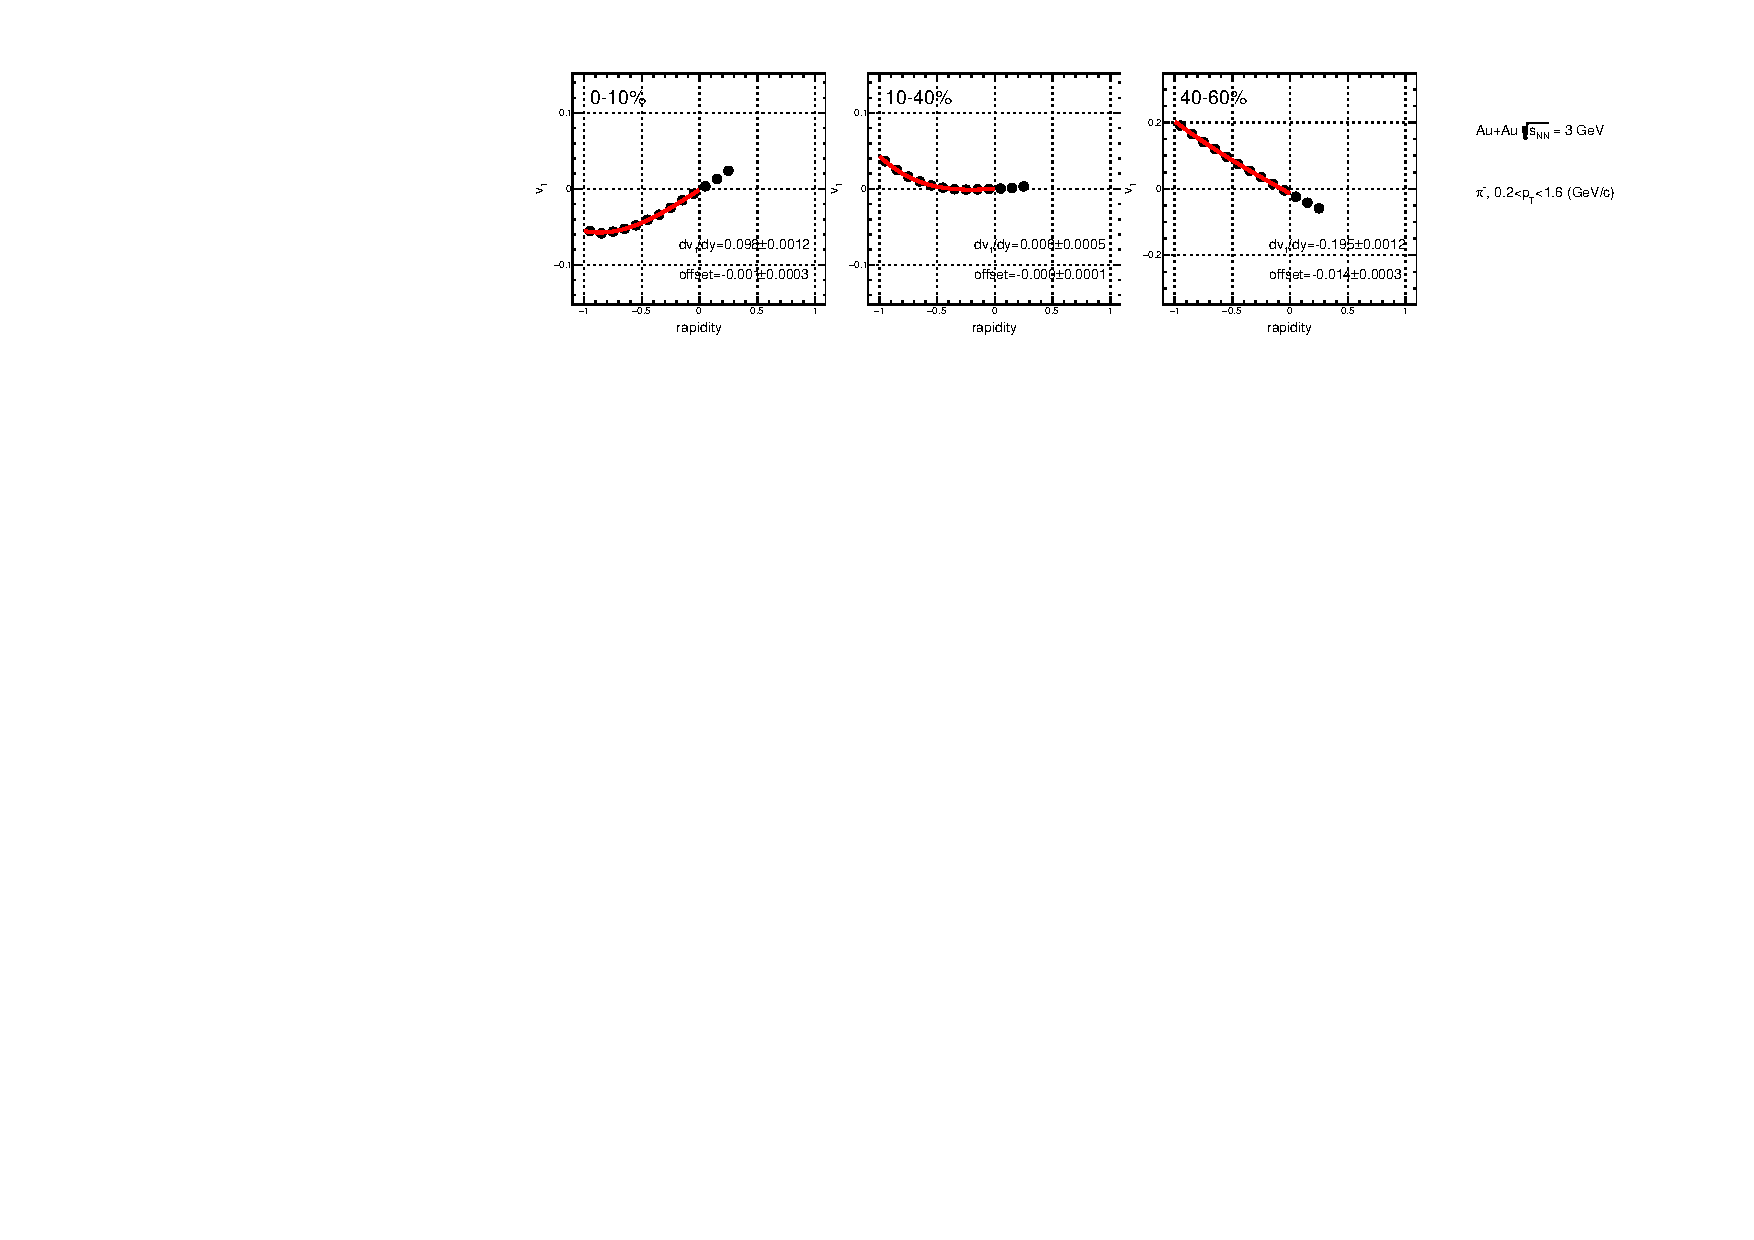
\includegraphics[scale=0.8]{chapter3/fig/v1ypikp/pionm_v1y_wide_cent.pdf}
\caption{\label{pion_v1y_widecent} pions' $v_{1}$ as a function of rapidity(y) in Au+Au collision at $\sqrt{s_{NN}}$=3GeV in 0-10\%, 10-40\% and 40-60\% bins.}
\end{figure}

\clearpage

Figure \ref{pion_v1pt_cent} shows $\pi^{+}$ and $\pi^{-}$ $v_{1}$ as a function of $p_{T}$ in different centrality bins. As we can see, pions $v_{1}$ is increasing with $p_{T}$ increasing. Figure \ref{pion_v1pt_widecent} also shows the results in the wider centrality bins. 

\begin{figure}[h]
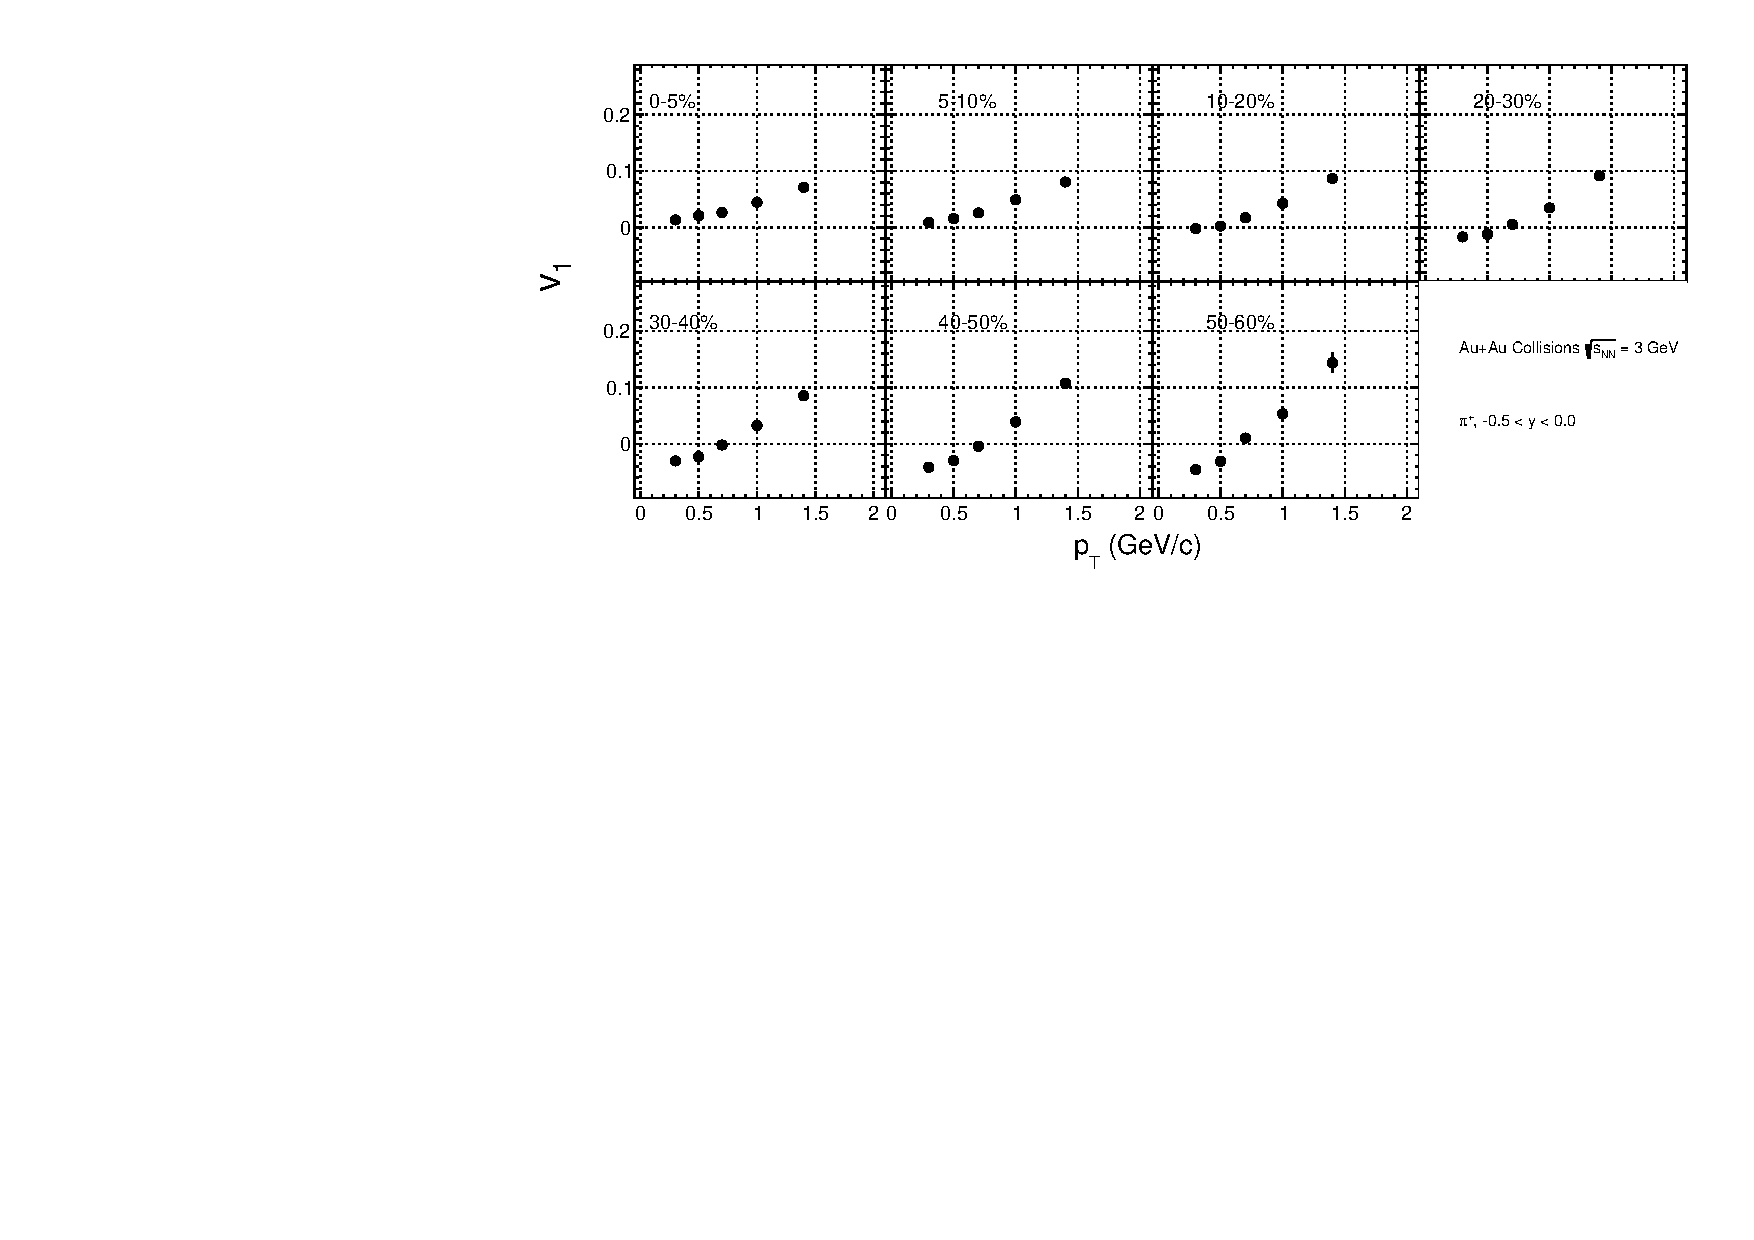
\includegraphics[scale=0.5]{chapter3/fig/v1ptpikp/v1pt_cent_pionp.pdf}
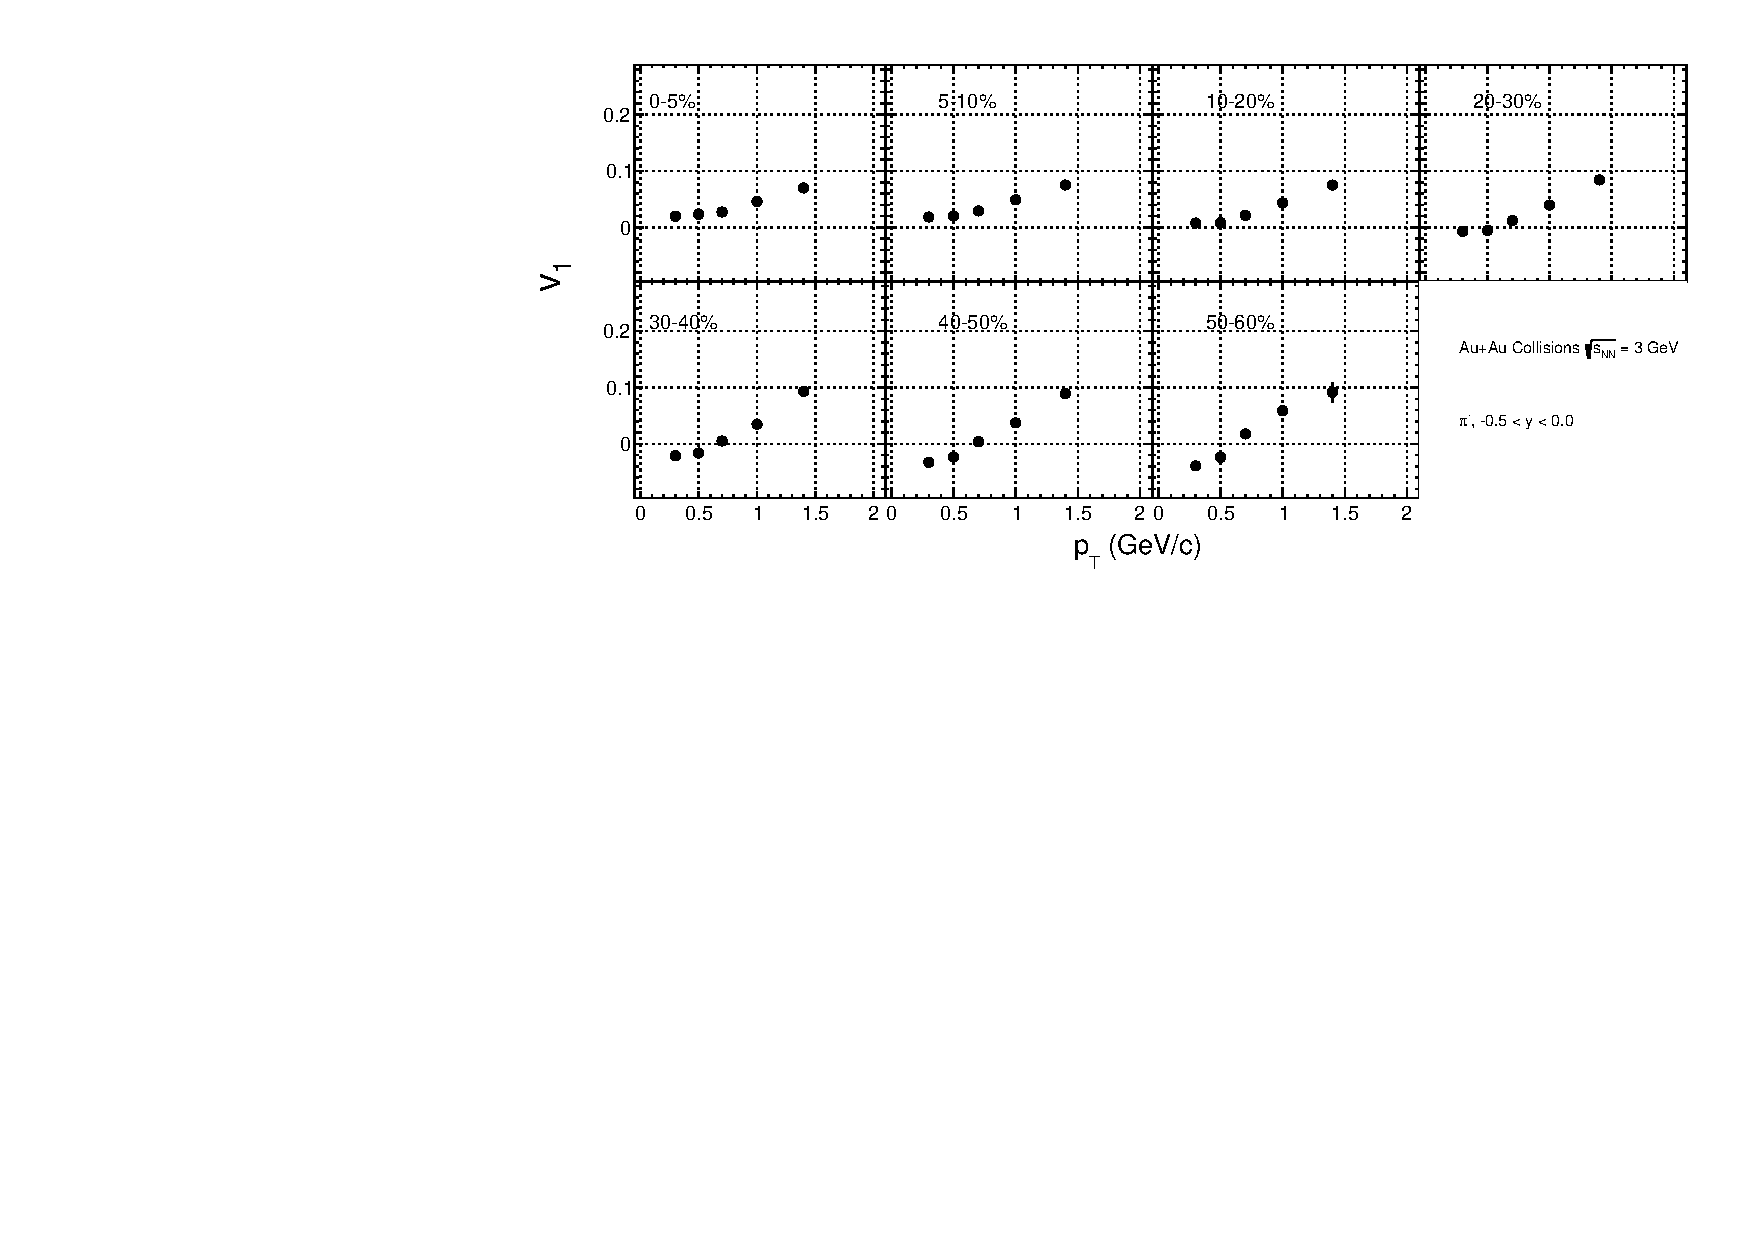
\includegraphics[scale=0.5]{chapter3/fig/v1ptpikp/v1pt_cent_pionm.pdf}
\caption{pions' $v_{1}$ as a function of transverse momentum ($p_{T}$) in Au+Au collisions at $\sqrt{s_{NN}}$ = 3 GeV.}
\label{pion_v1pt_cent}
\end{figure}

\begin{figure}[h]
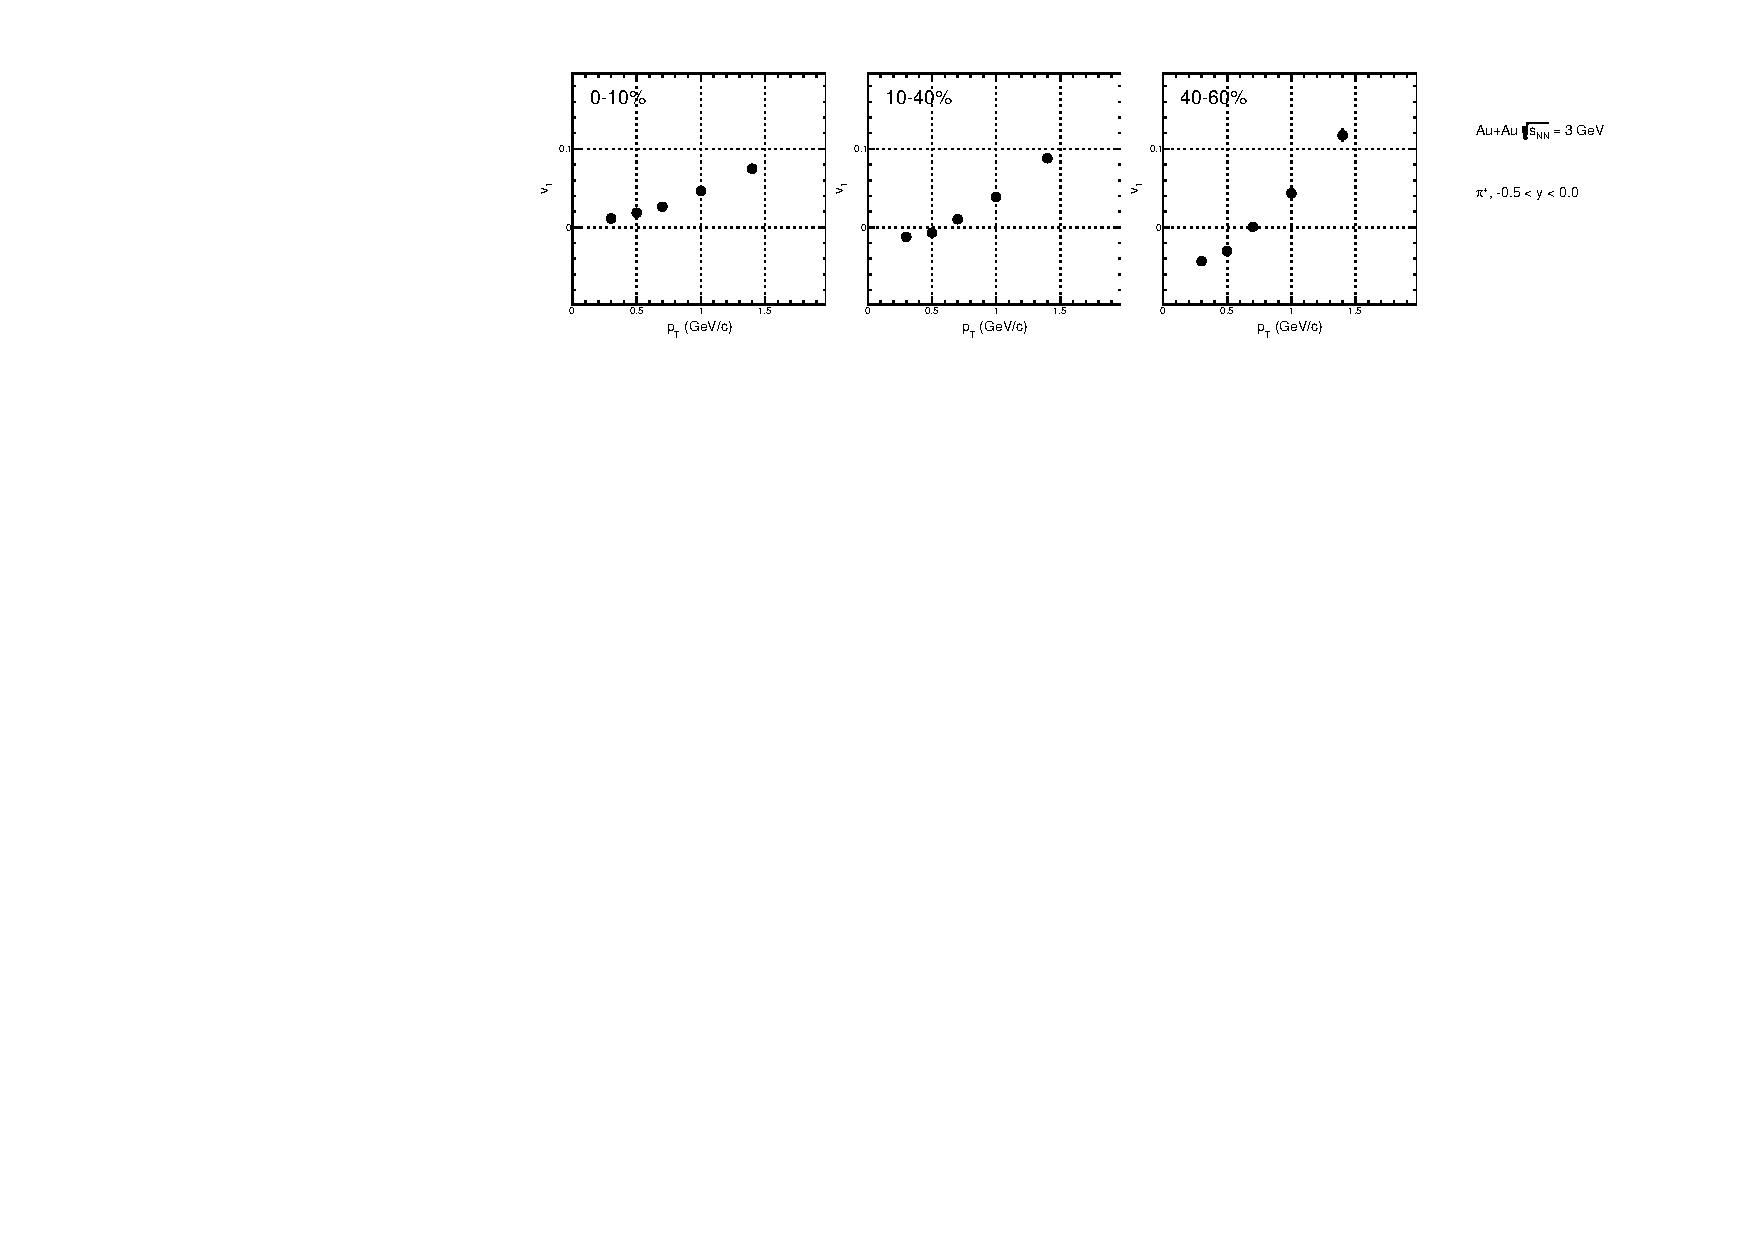
\includegraphics[scale=0.5]{chapter3/fig/v1ptpikp/pionp_v1pt_wide_cent.pdf}
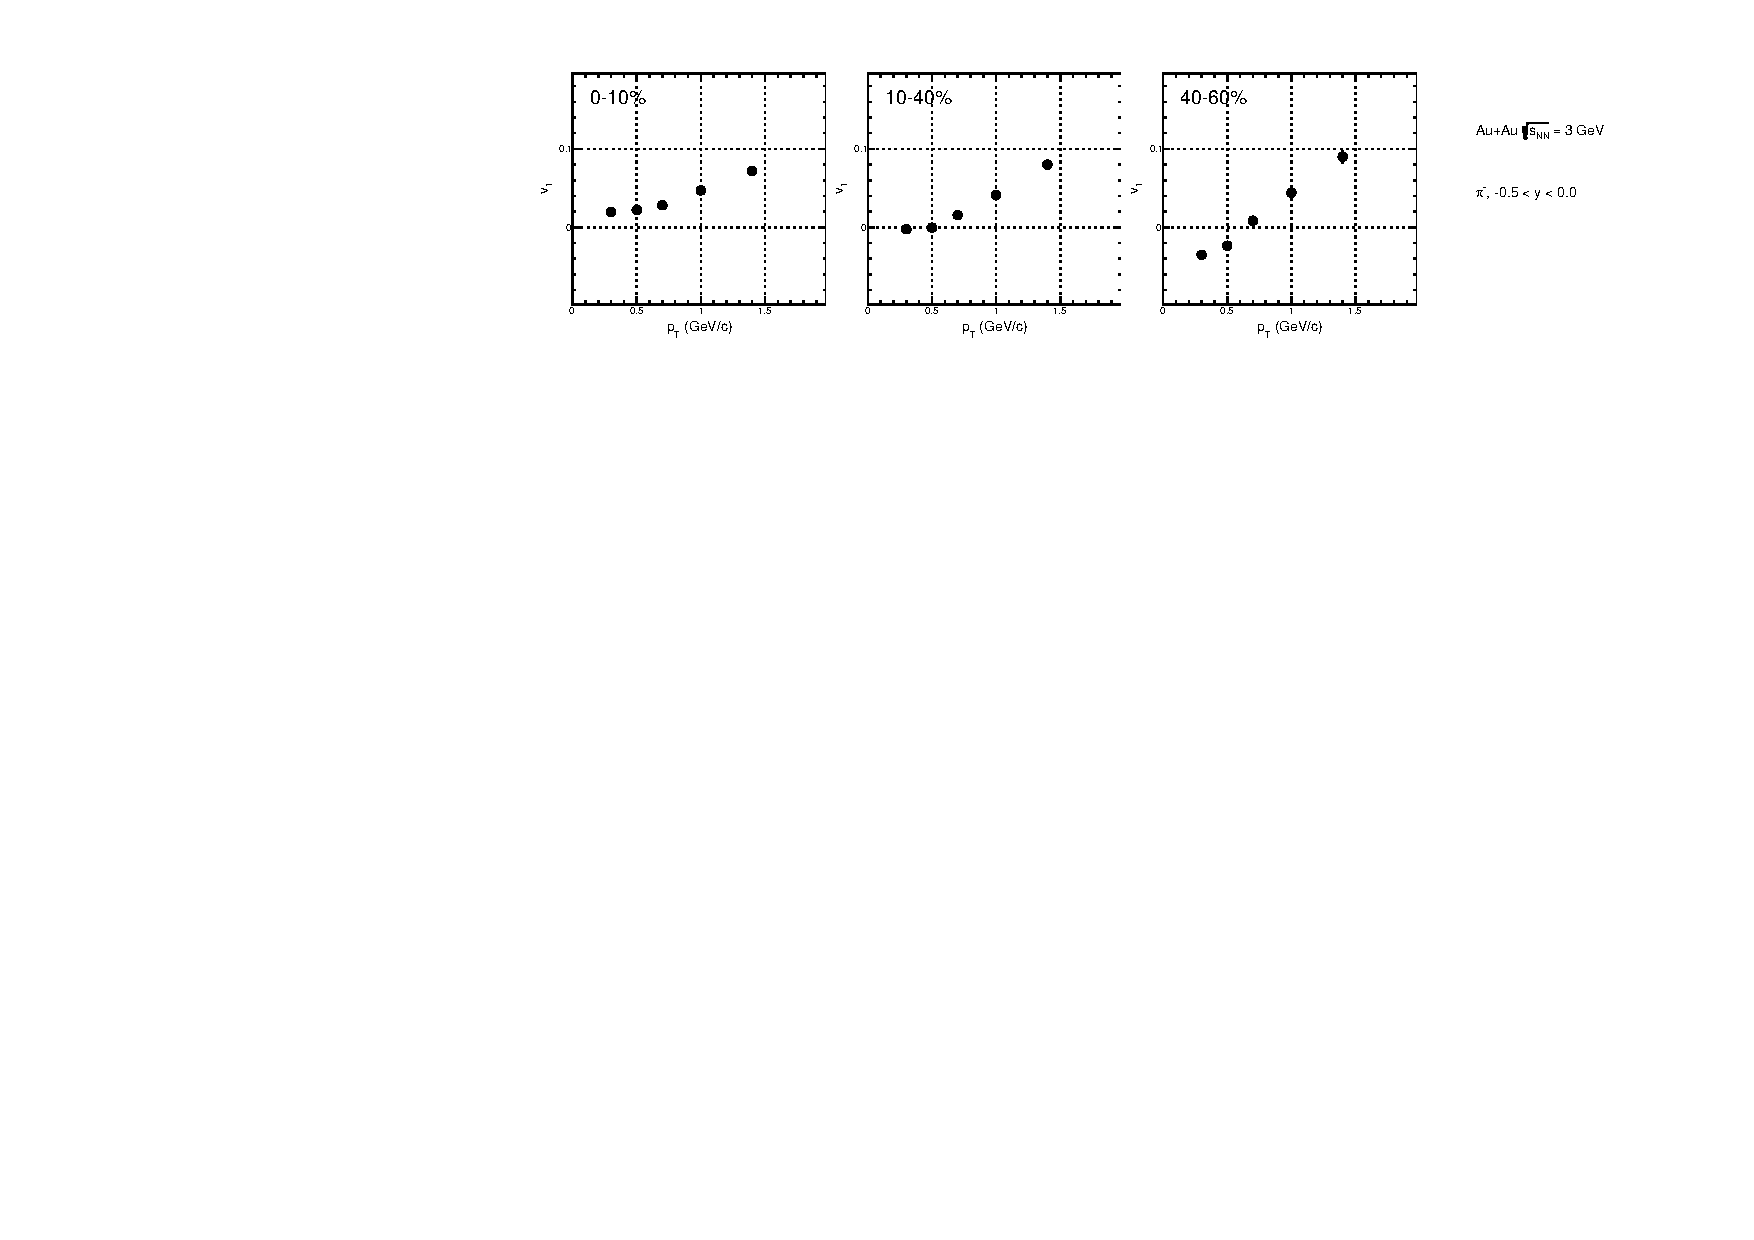
\includegraphics[scale=0.5]{chapter3/fig/v1ptpikp/pionm_v1pt_wide_cent.pdf}
\caption{pions' $v_{1}$ as a function of transverse momentum ($p_{T}$) in Au+Au collisions at $\sqrt{s_{NN}}$ = 3 GeV in 0-10\%, 10-40\% and 40-60\% centrality bins.}
\label{pion_v1pt_widecent}
\end{figure}

\clearpage

\subsubsection{kaons' $v_{1}$ as a function of $p_{T}$ and rapidity}
Figure \ref{kaon_v1y_cent} shows $K^{+}, K^{-}$ $v_{1}$ as a function of y for different centrality bins from 0-5\% to 50-60\%, The red line is fitting function \ref{fit_v1_formula}, $p_{T}$ range is [0.4, 1.6] GeV/c, which is same with STAR BES-I results. As we can see, the magnitude of kaons' $v_{1}$ has weak centrality dependence, which is not same with pions' case, this might be due to kaon has smaller hadronic scattering cross section than pions, and the $v_{1}$ between $K^{+}$ and $K^{-}$ is very similar, figure \ref{kaon_dv1dy_cent} shows $K^{+}, K^{-}$ $dv_{1}/dy$ as a function of centrality. In order to make comparison to STAR BES-I results, we have these results in wider centrality bin in the figure \ref{kaon_v1y_widecent}. And their $v_{1}$ slope is decreasing from central collision to peripheral collision.


\begin{figure}[h]
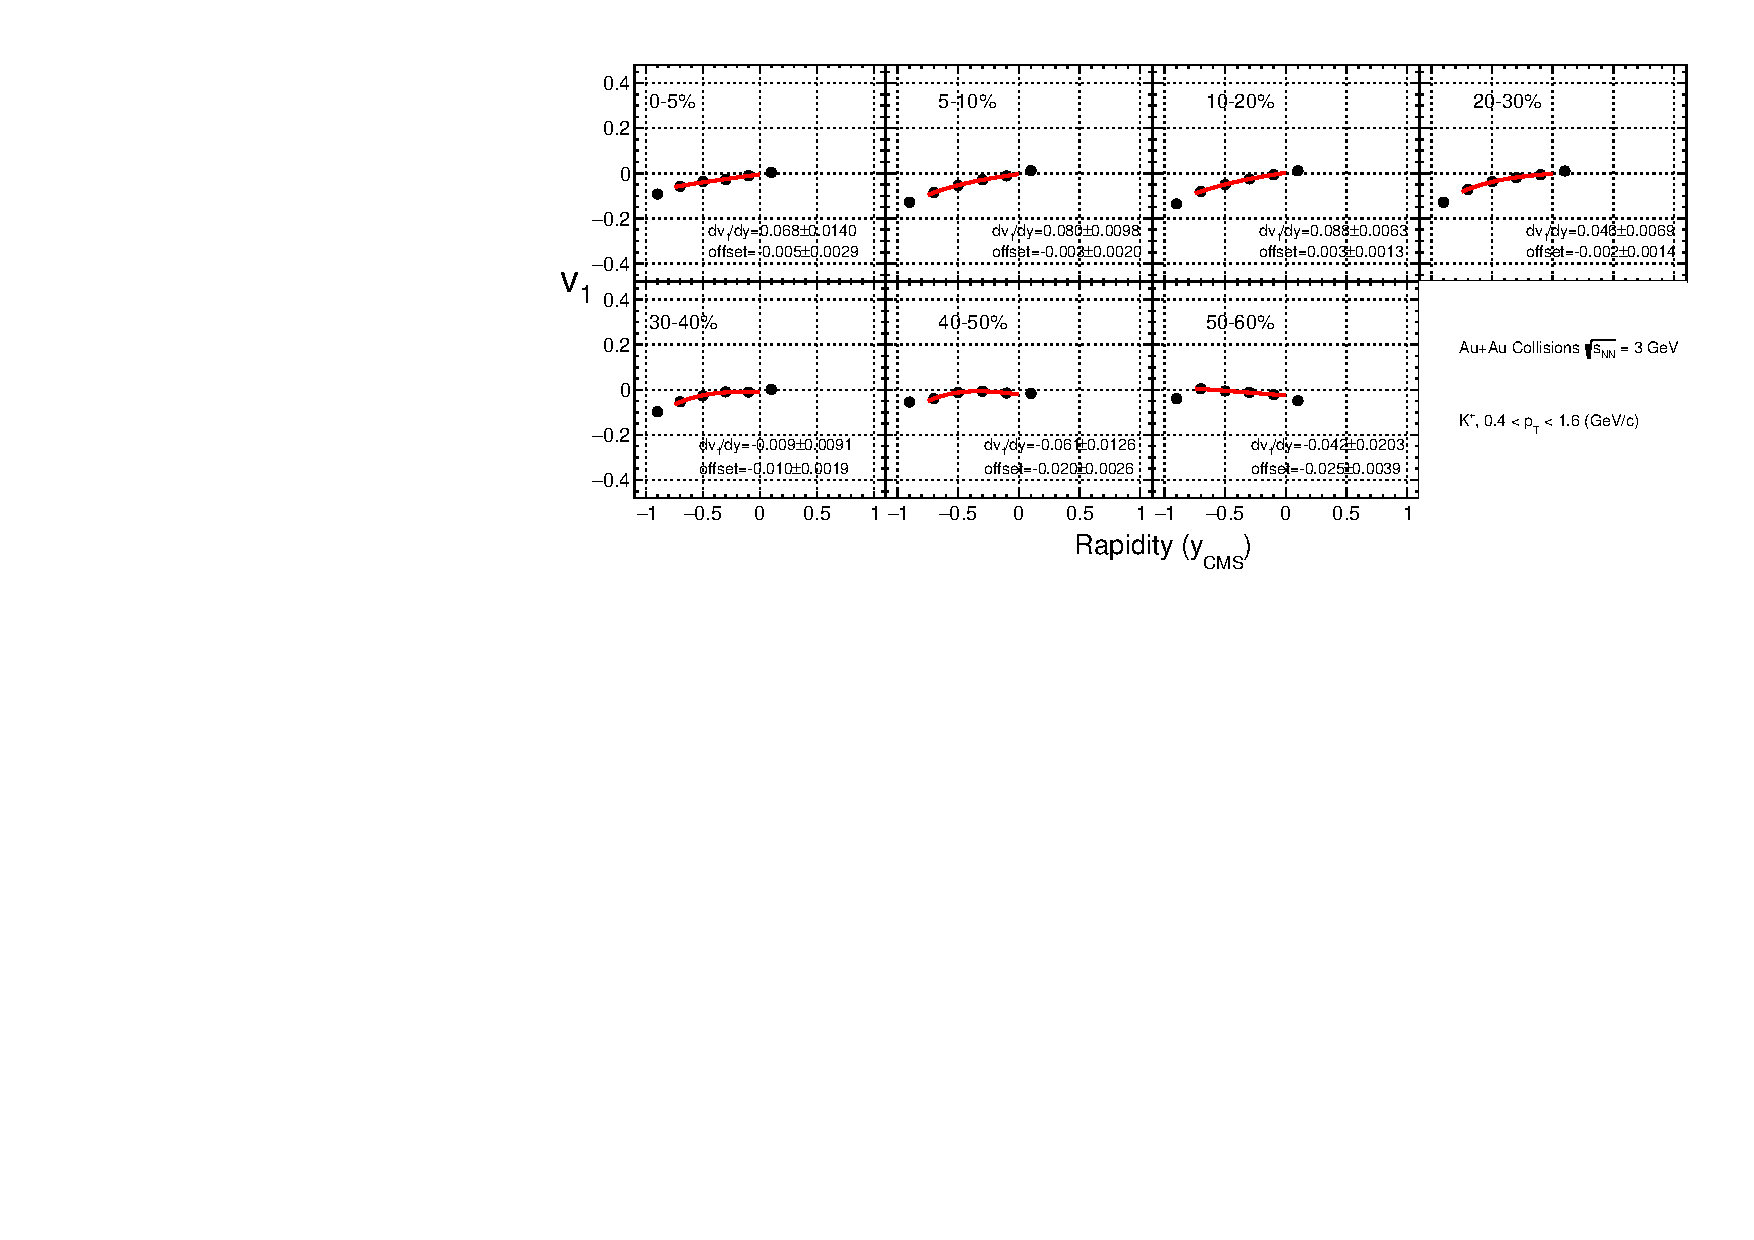
\includegraphics[scale=0.5]{chapter3/fig/v1ypikp/v1kaonp_cent.pdf}
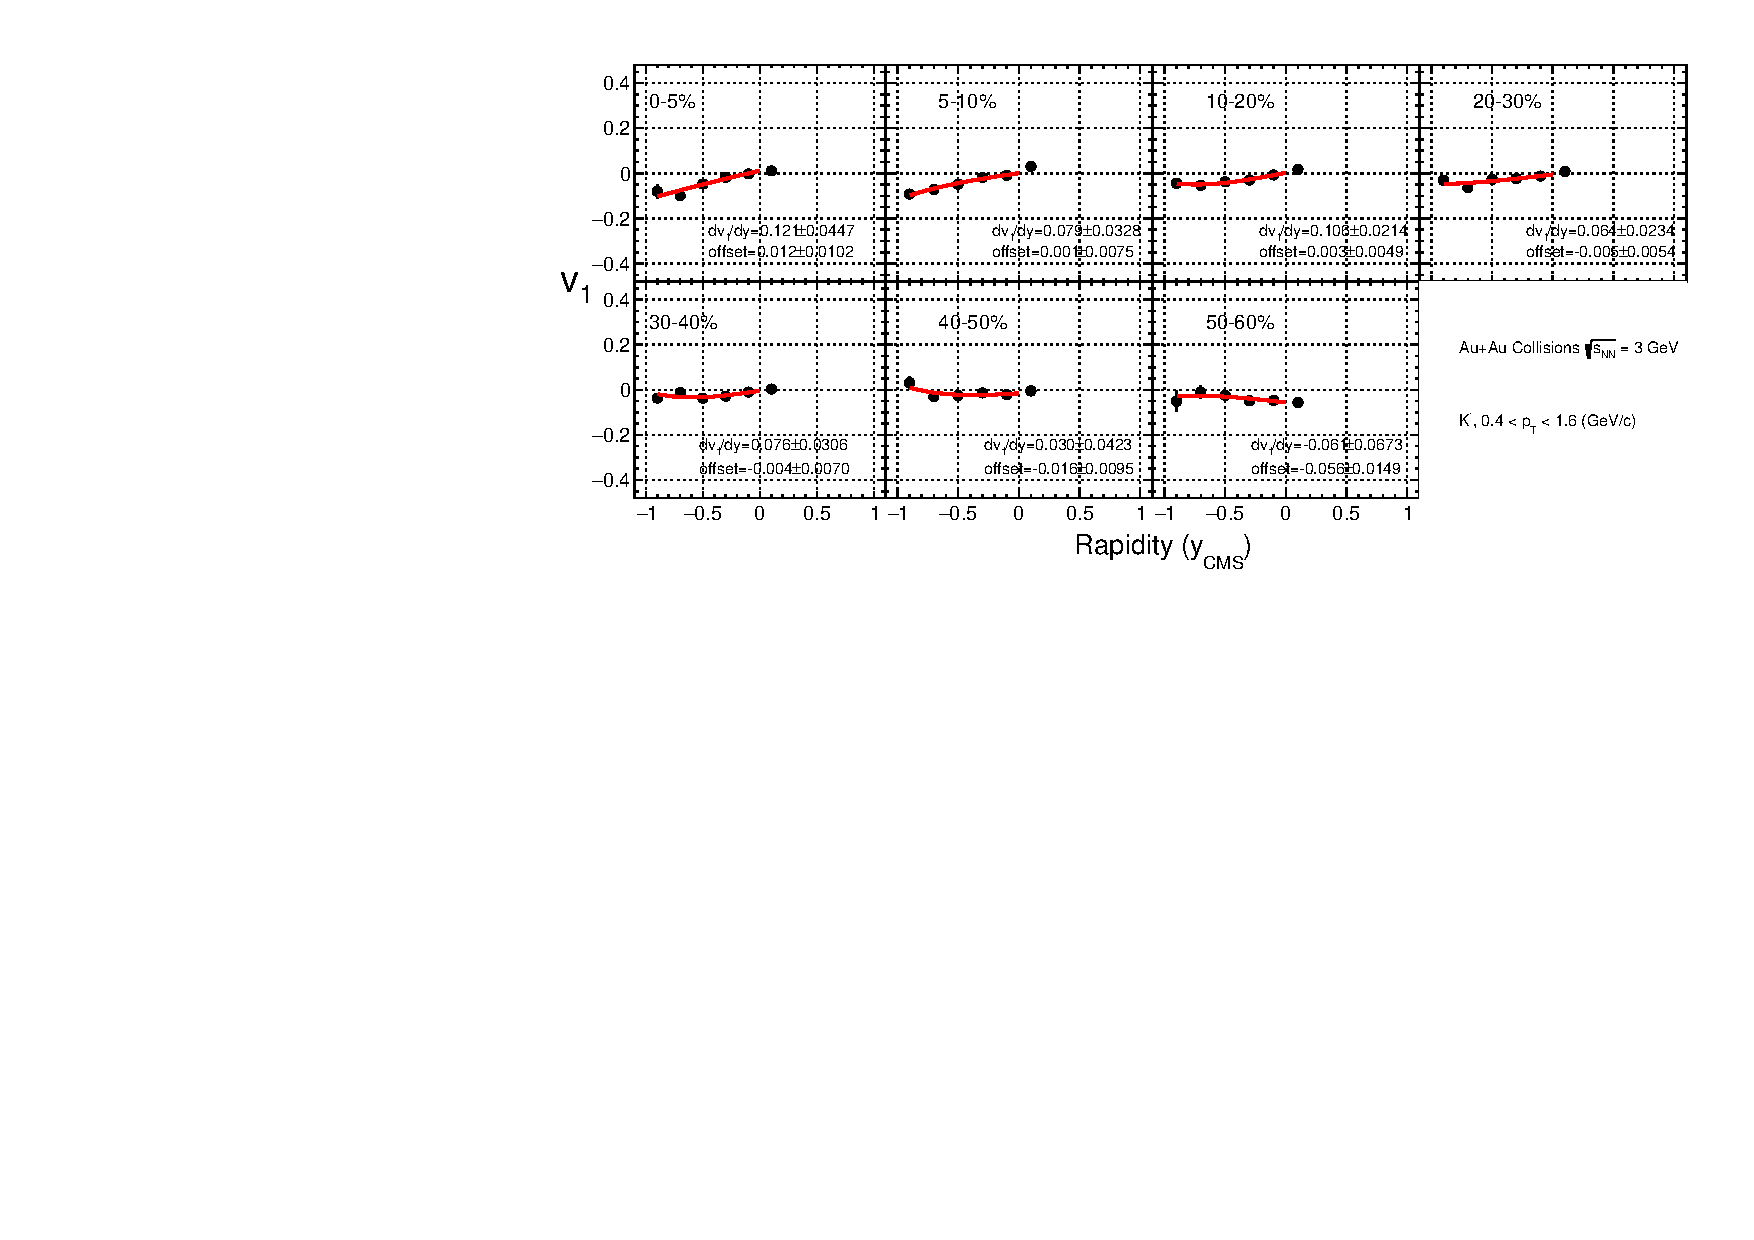
\includegraphics[scale=0.5]{chapter3/fig/v1ypikp/v1kaonm_cent.pdf}
\caption{\label{kaon_v1y_cent} $v_{1}$ as a function of rapidity(y) in different centrality bins for $K^{+}$ and $K^{-}$ in Au+Au collisions at $\sqrt{s_{NN}}$. The red line is fitting function.}
\end{figure}

\begin{figure}[h]
\centering
\subfigure{   
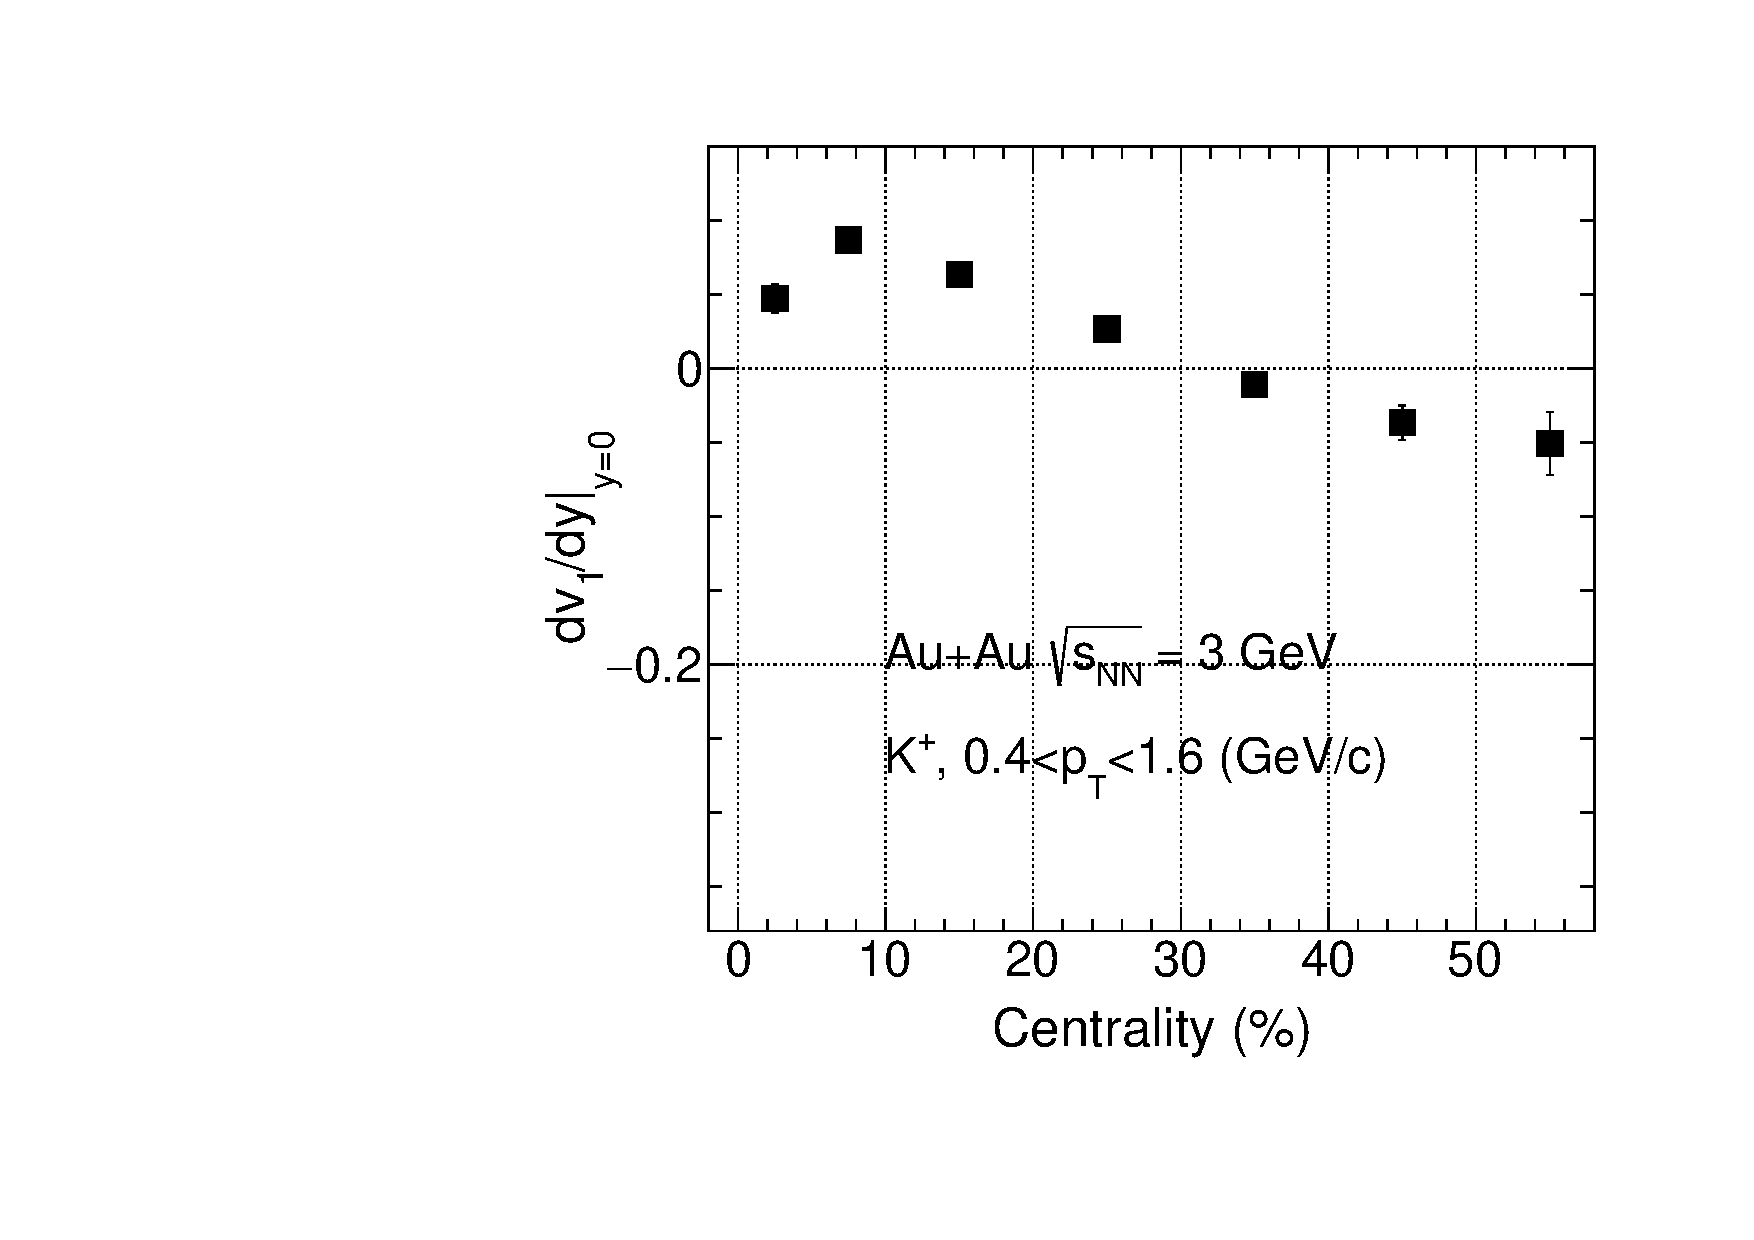
\includegraphics[width=0.4\textwidth]{chapter3/fig/v1ypikp/dv1dy_kaonp.pdf}}
\subfigure{
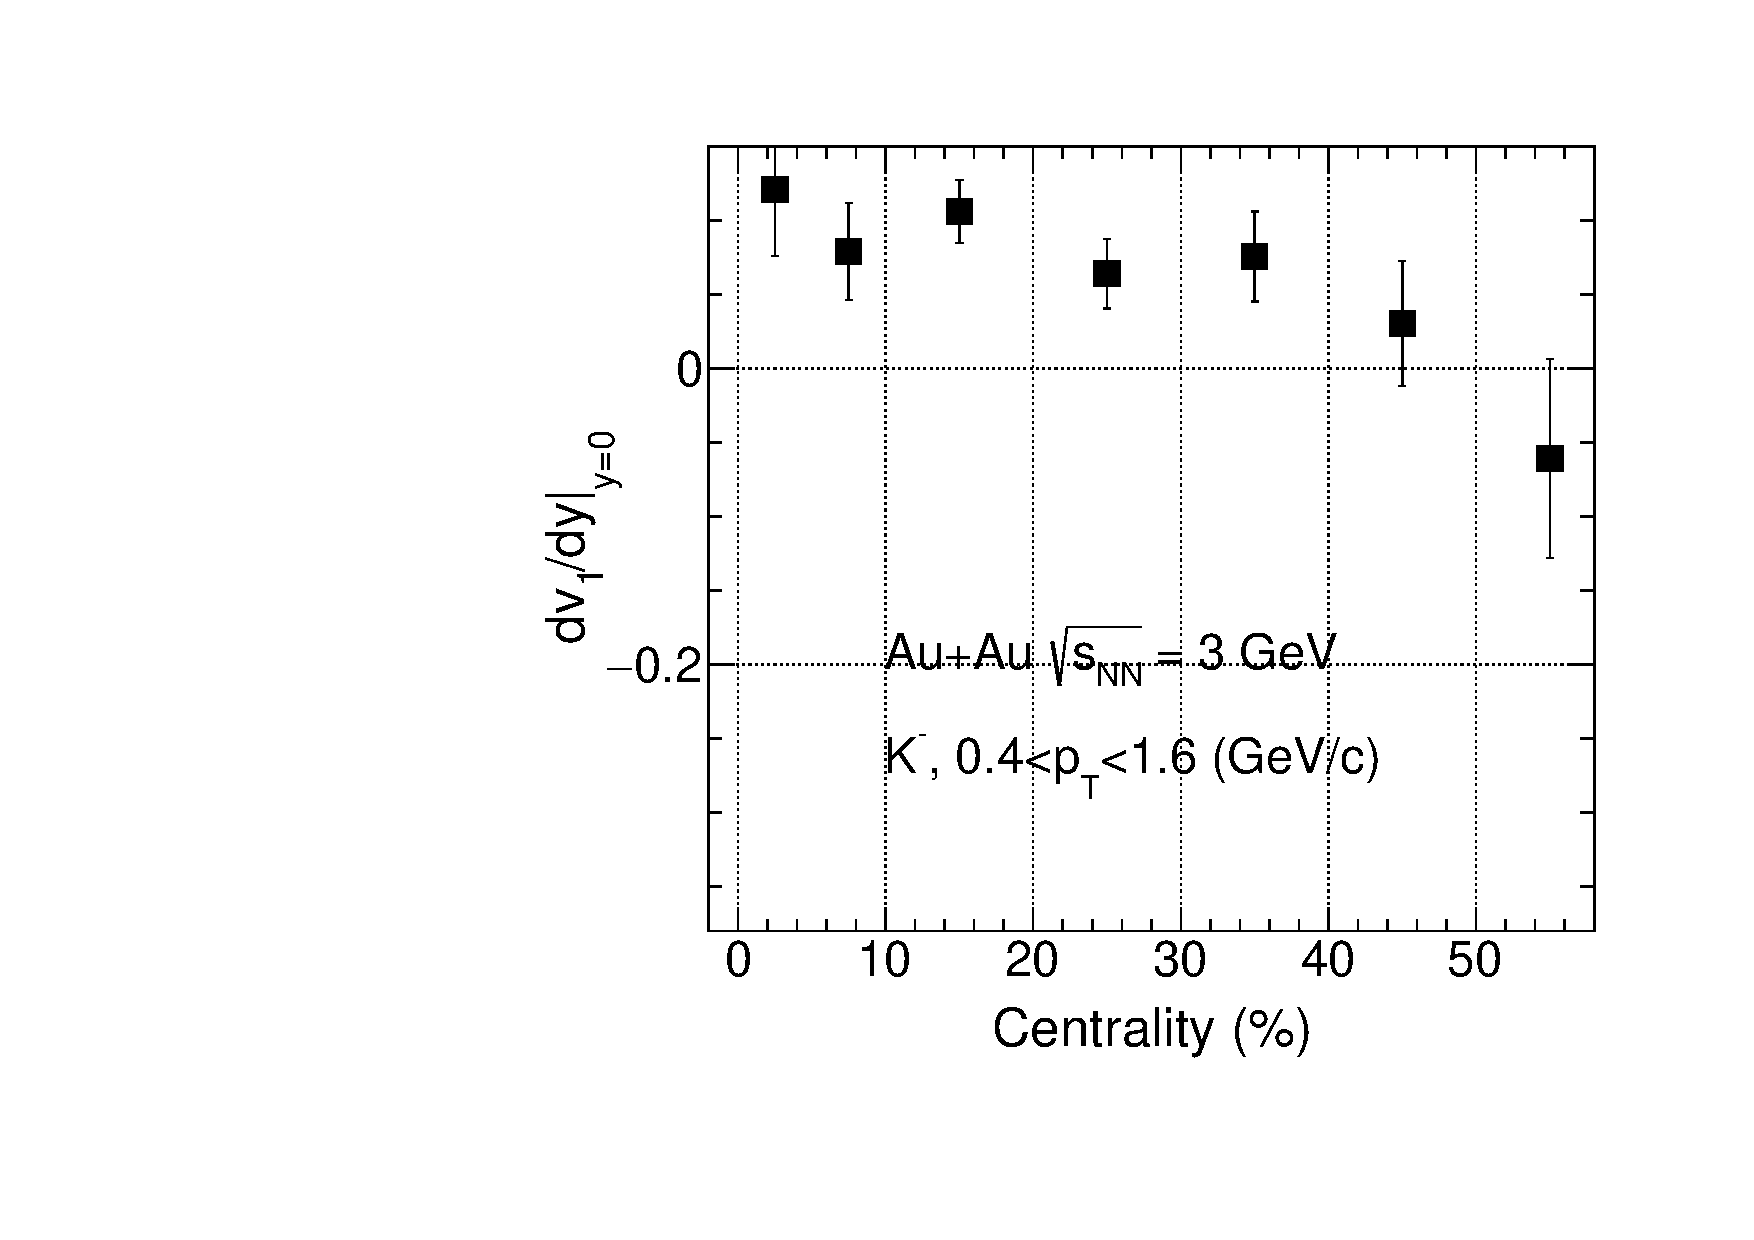
\includegraphics[width=0.4\textwidth]{chapter3/fig/v1ypikp/dv1dy_kaonm.pdf}}
\caption{\label{kaon_dv1dy_cent} kaons' $v_{1}$ slope $dv_{1}/dy$ as a function of centrality, (left) $K^{+}$ (right) $K^{-}$ in Au+Au collisions $\sqrt{s_{NN}}$ = 3GeV.}
\end{figure}

\begin{figure}[h]
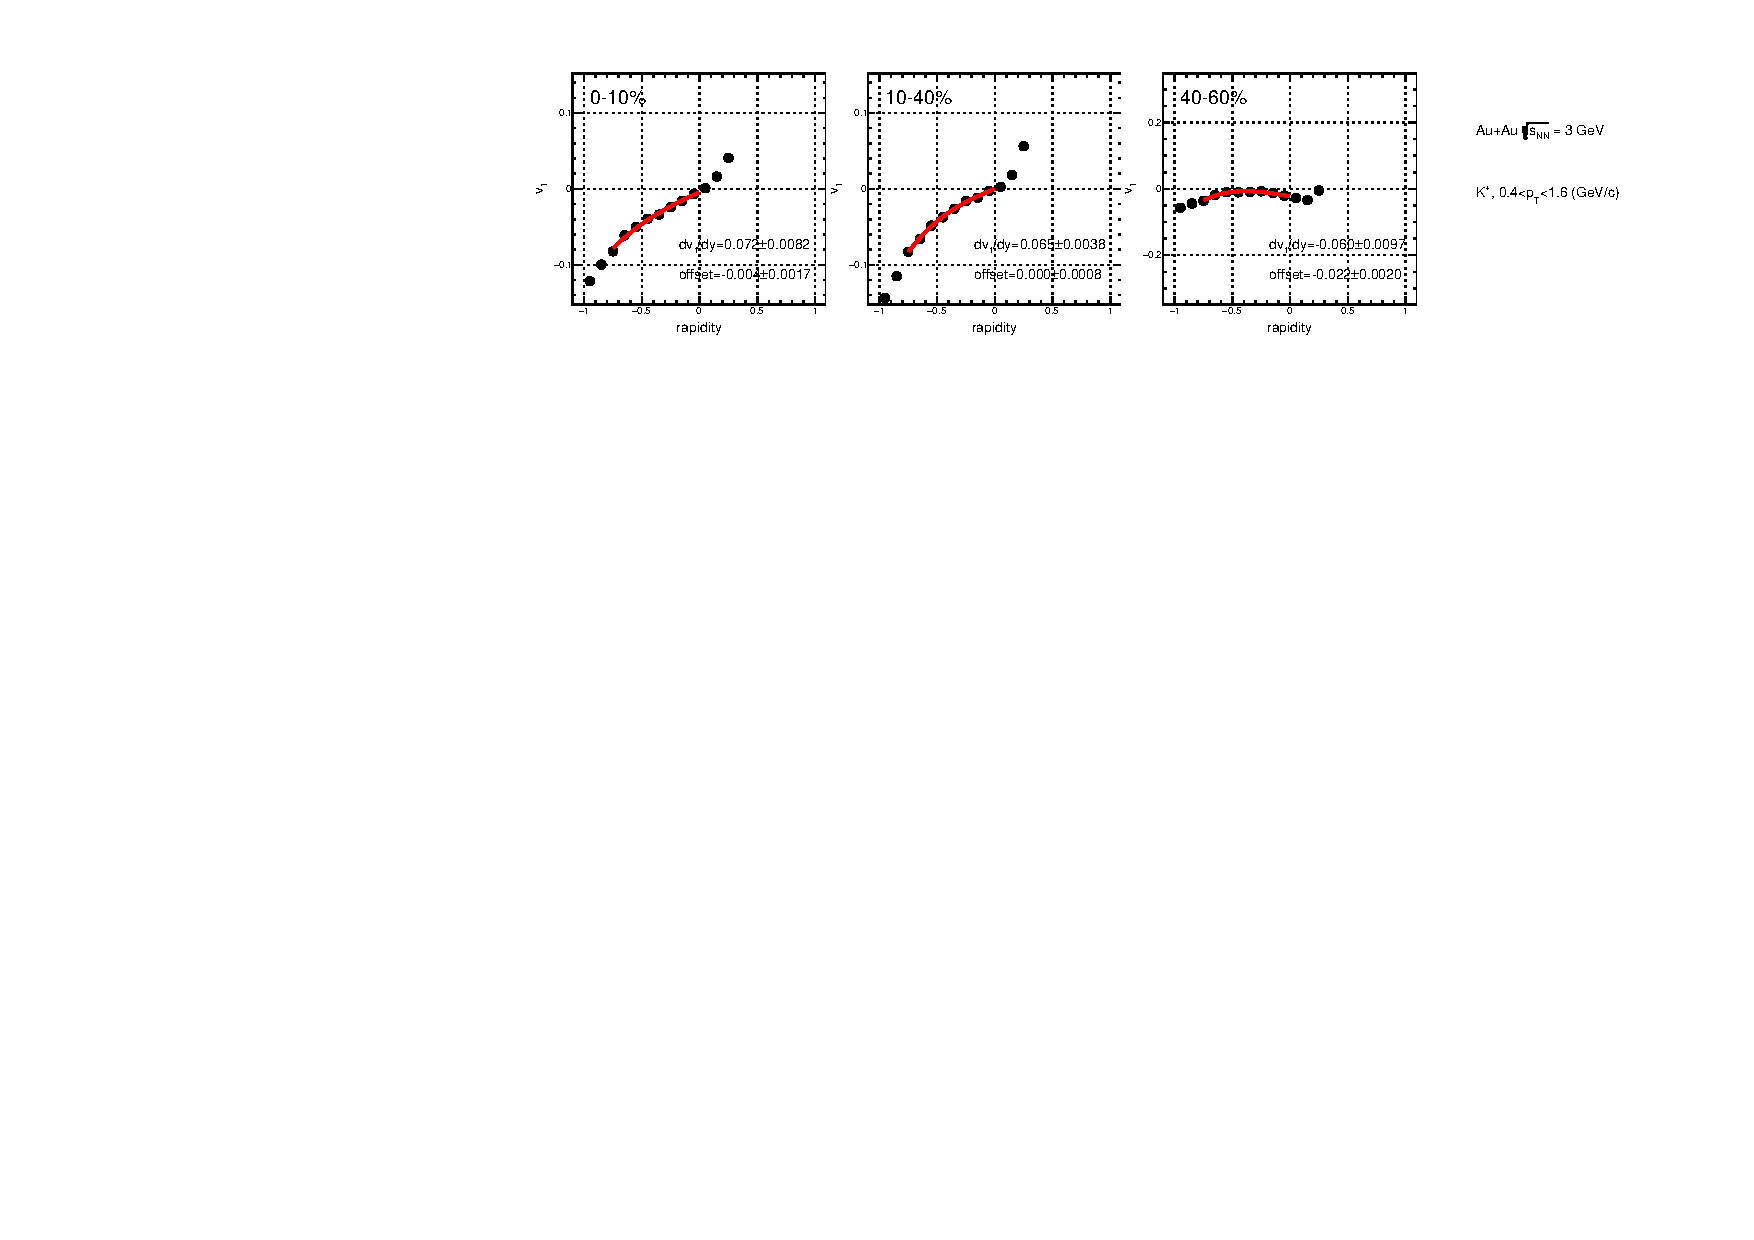
\includegraphics[scale=0.8]{chapter3/fig/v1ypikp/kaonp_v1y_wide_cent.pdf}
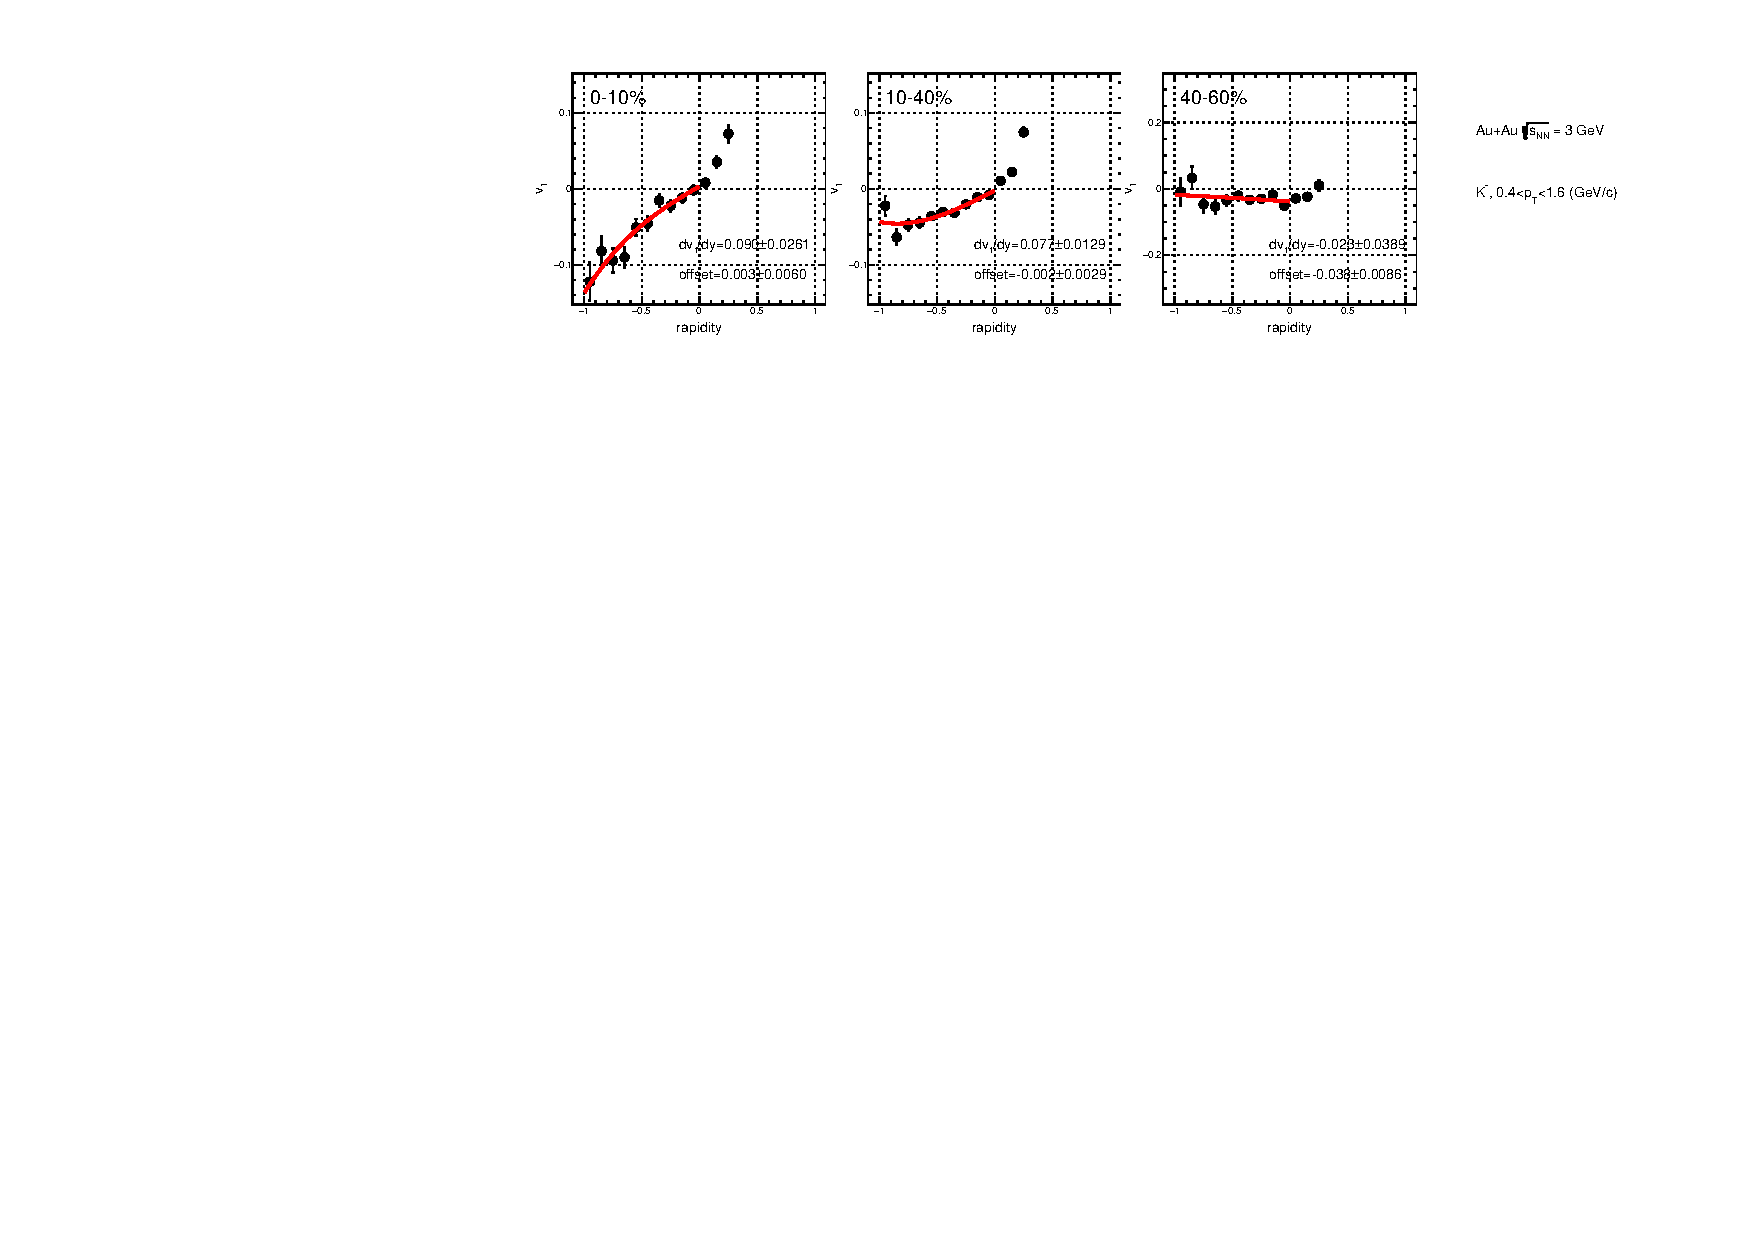
\includegraphics[scale=0.8]{chapter3/fig/v1ypikp/kaonm_v1y_wide_cent.pdf}
\caption{\label{kaon_v1y_widecent} kaons' $v_{1}$ as a function of rapidity(y) in Au+Au collision at $\sqrt{s_{NN}}$=3GeV in 0-10\%, 10-40\% and 40-60\% bins.}
\end{figure}

\clearpage

We also study the $p_{T}$ dependence of kaons' $v_{1}$ in the mid-rapidity region (-0.5$<$y$<$0) in different centrality bins in the figure \ref{kaon_v1pt_cent}.As we can see, kaons $v_{1}$ is increasing with $p_{T}$ increasing. Figure \ref{kaon_v1pt_widecent} also shows the results in the wider centrality bins. 

\begin{figure}[h]
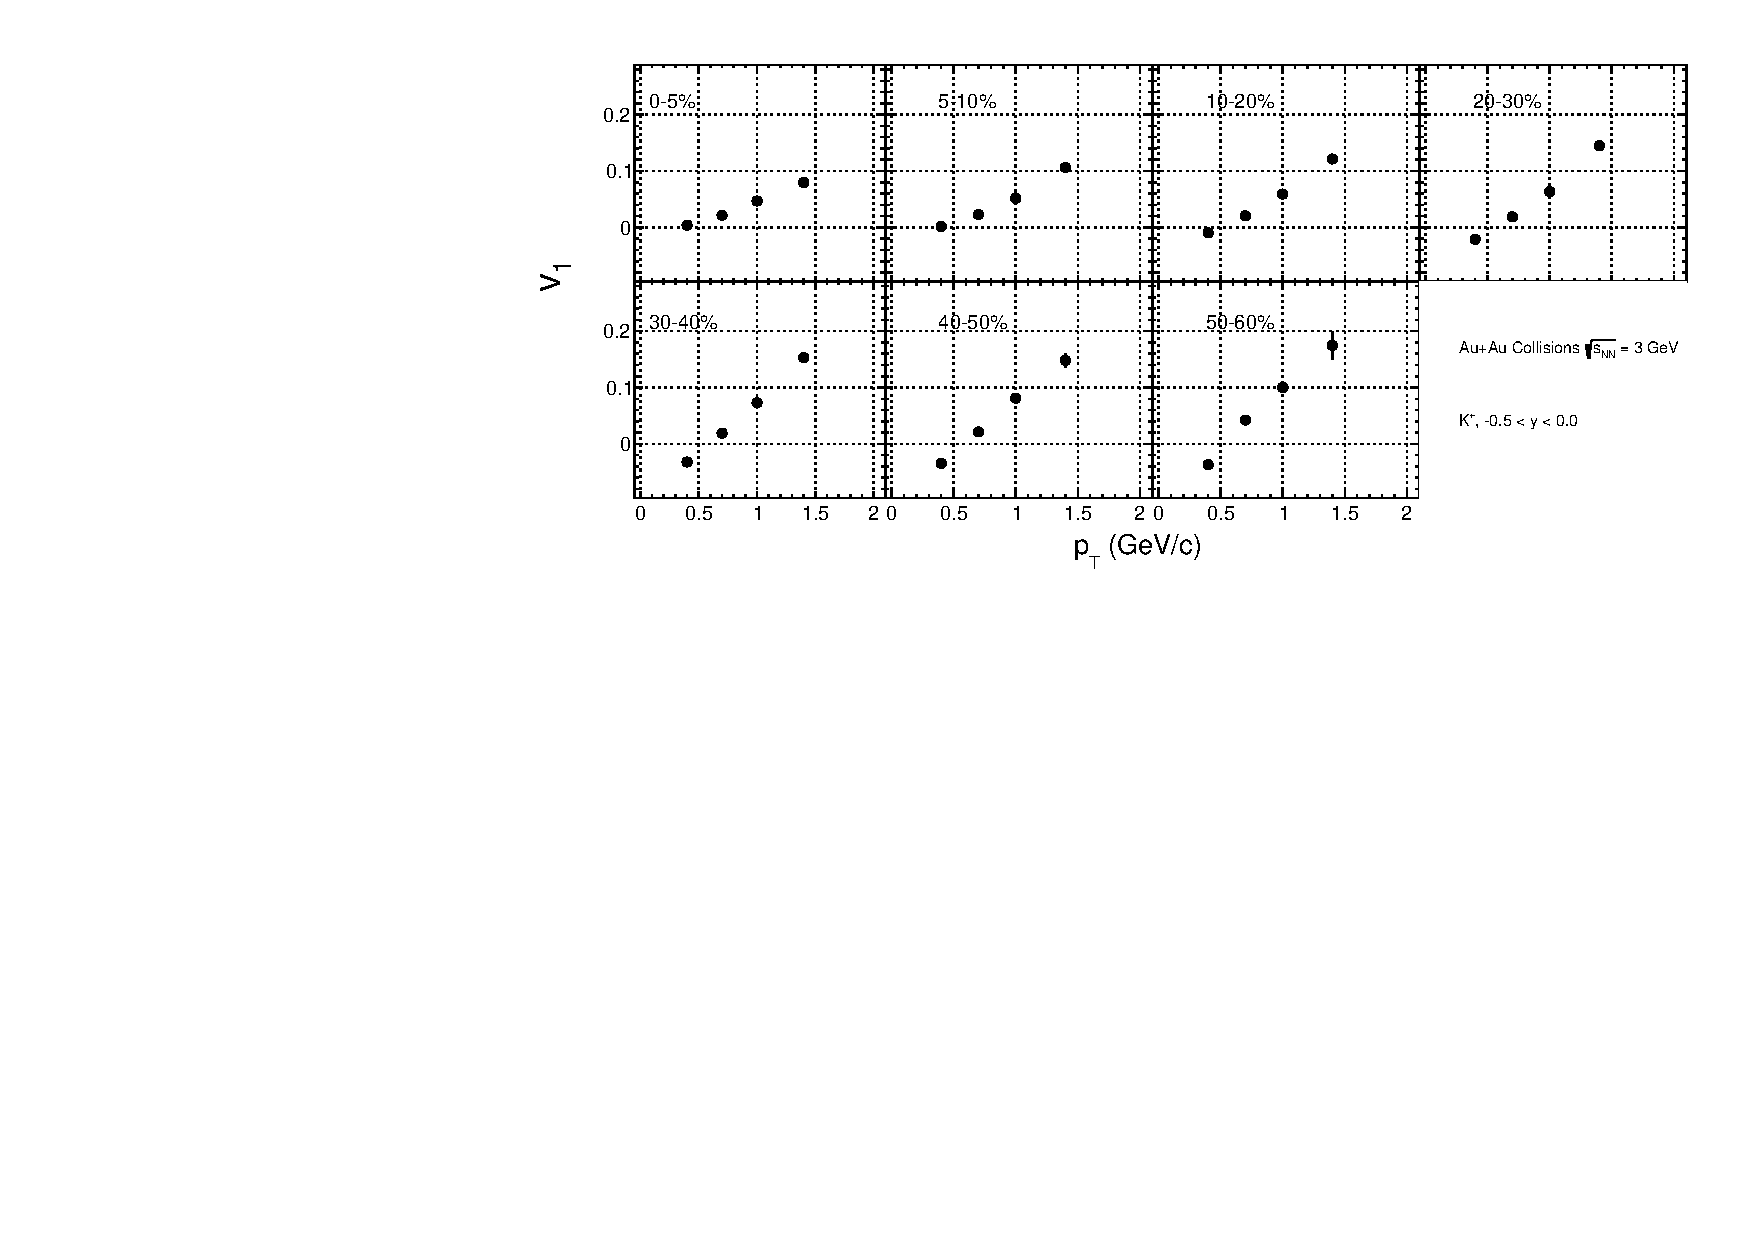
\includegraphics[scale=0.5]{chapter3/fig/v1ptpikp/v1pt_cent_kaonp.pdf}
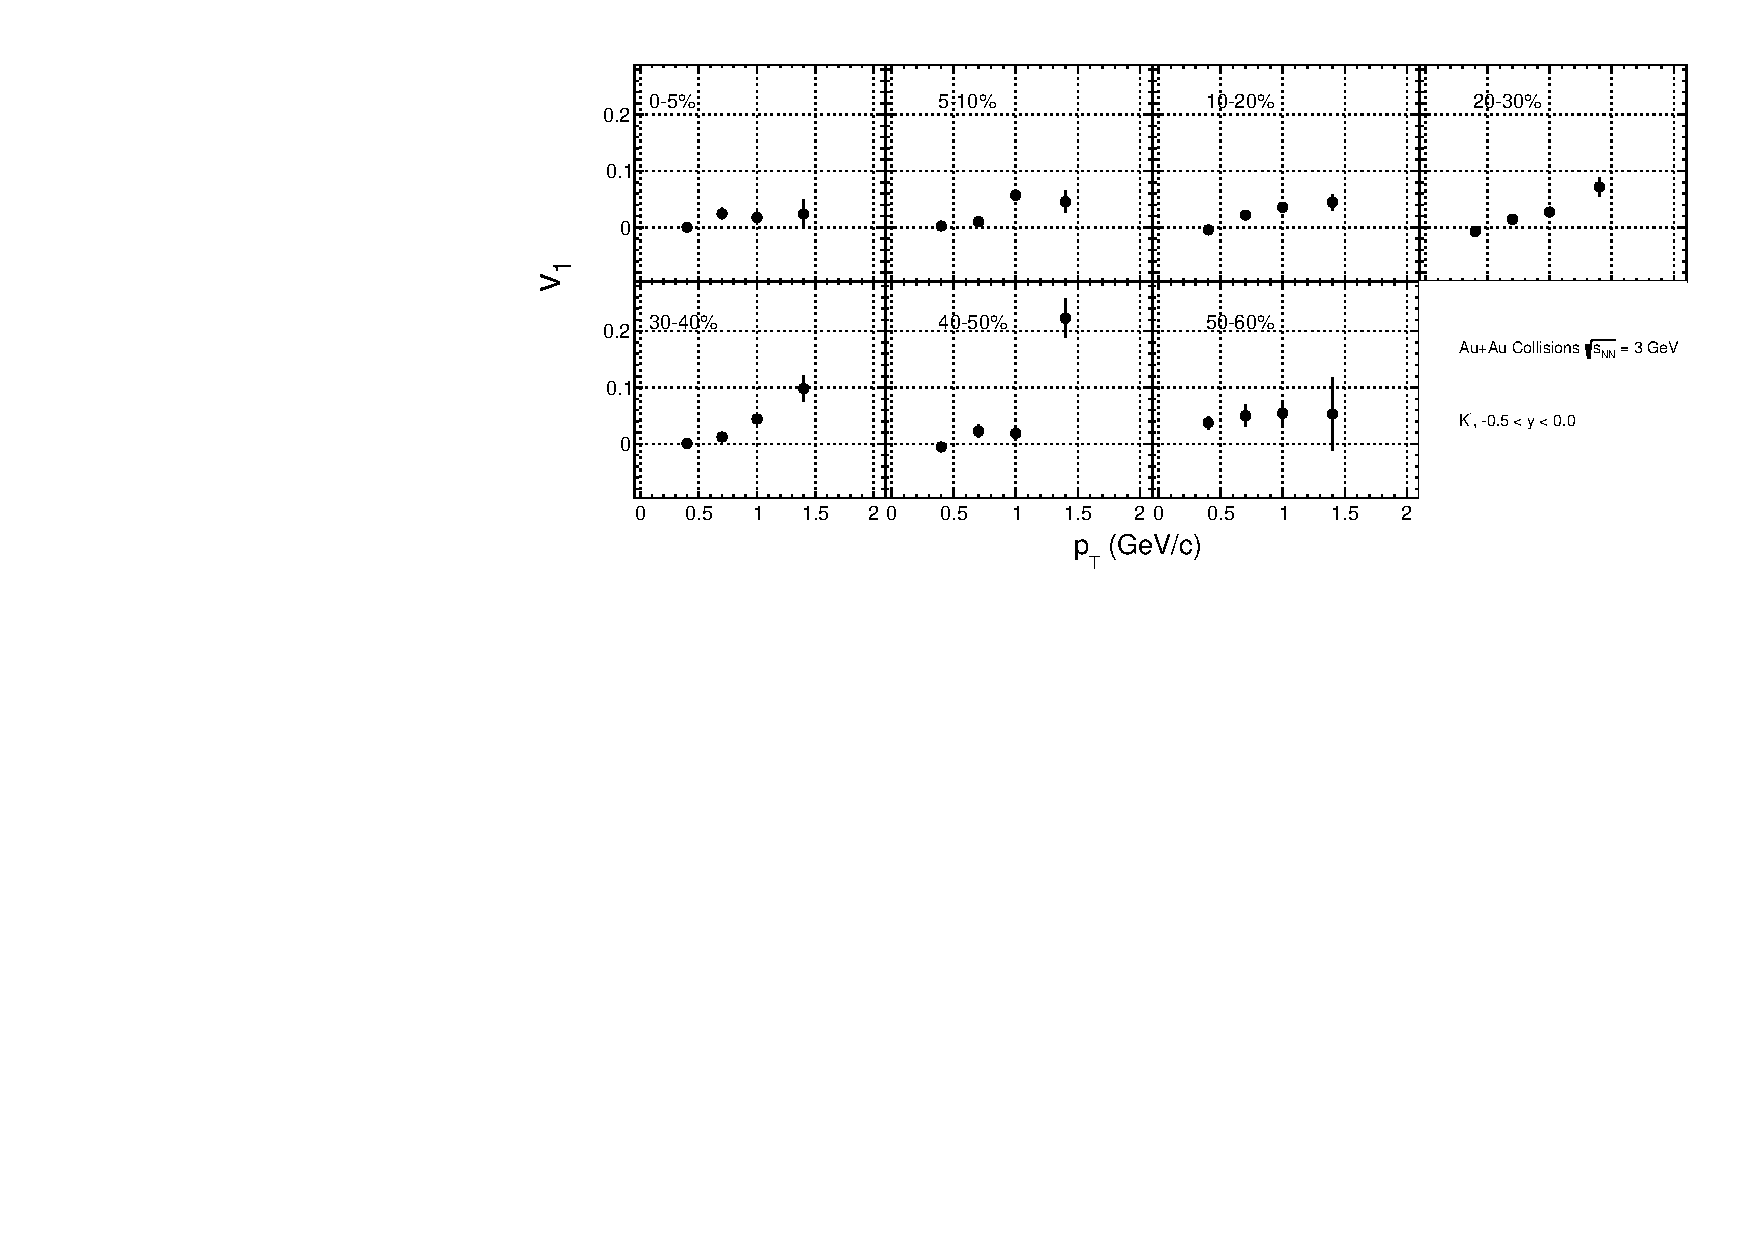
\includegraphics[scale=0.5]{chapter3/fig/v1ptpikp/v1pt_cent_kaonm.pdf}
\caption{kaons' $v_{1}$ as a function of transverse momentum ($p_{T}$) in Au+Au collisions at $\sqrt{s_{NN}}$ = 3 GeV.}
\label{kaon_v1pt_cent}
\end{figure}

\begin{figure}[h]
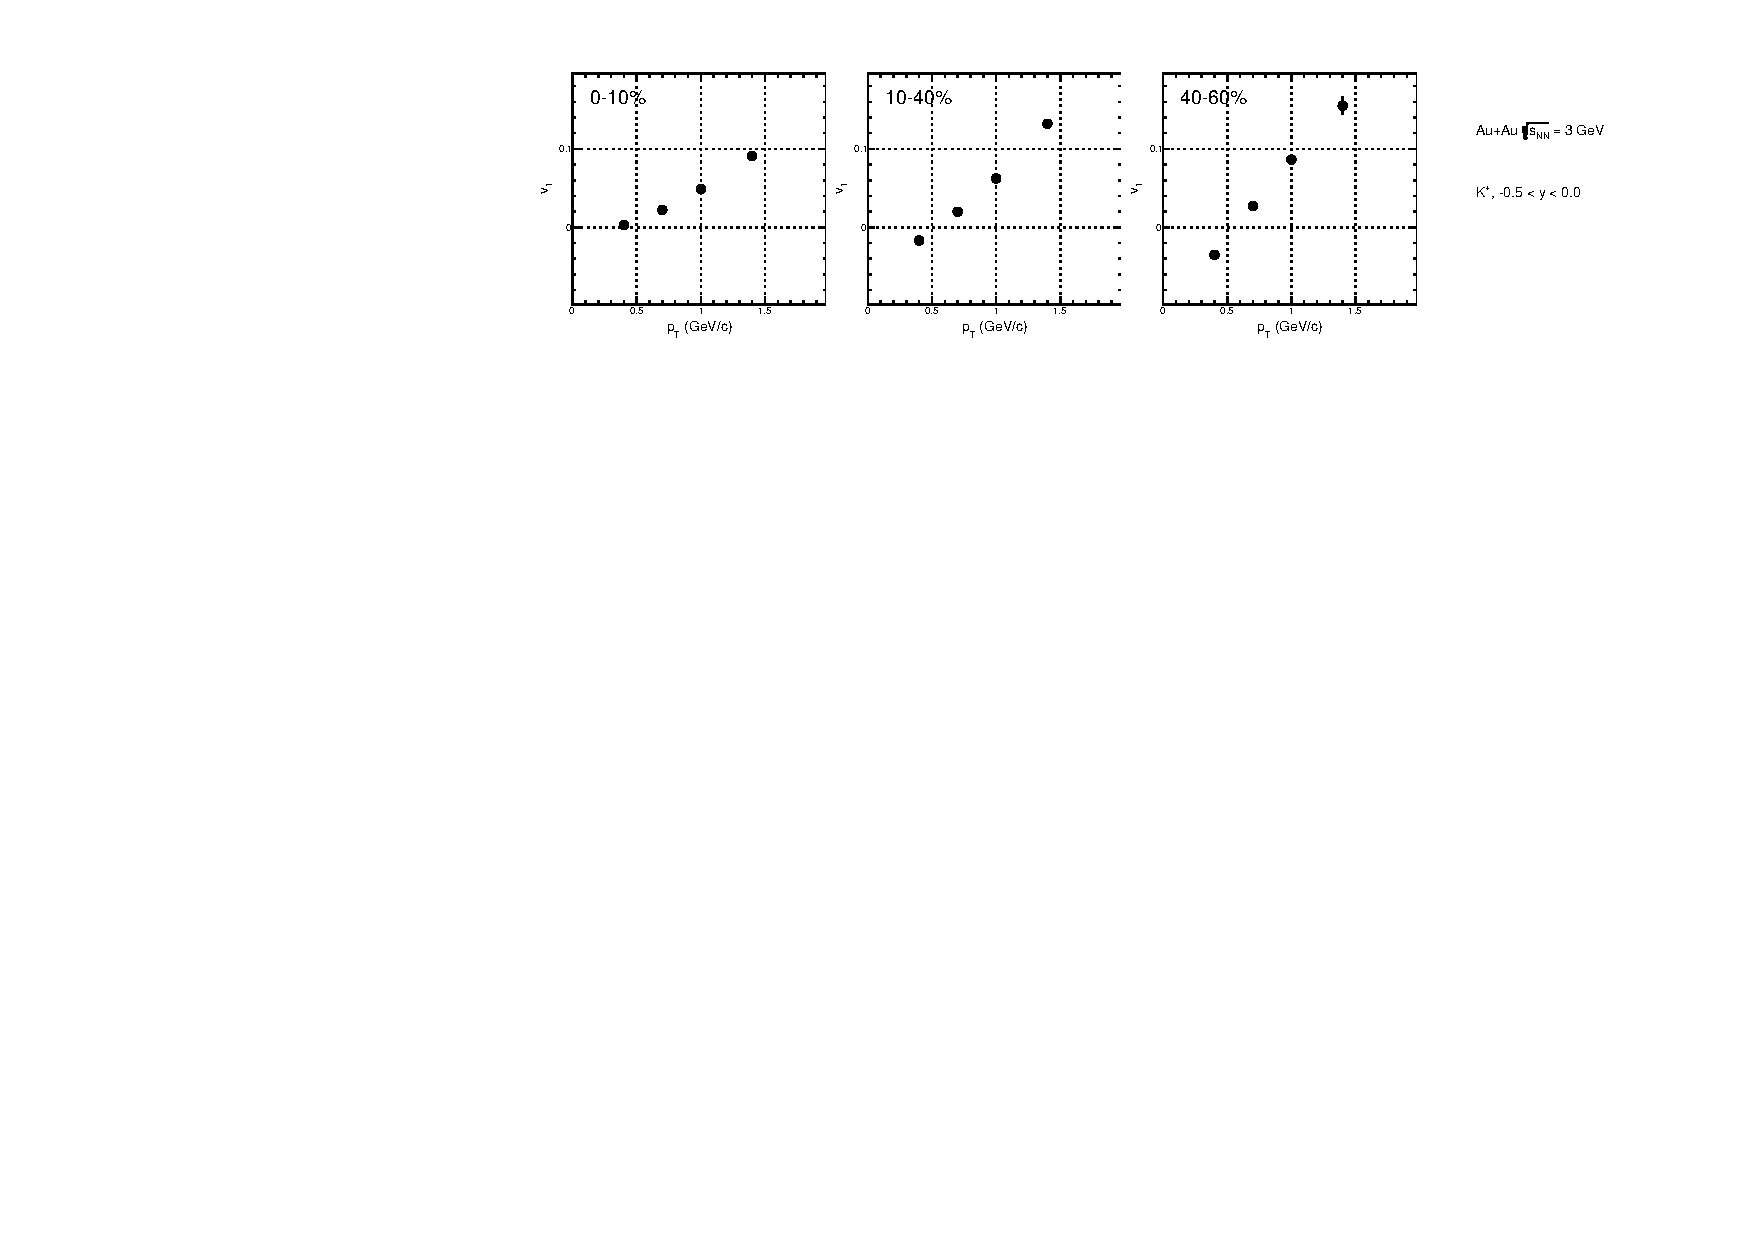
\includegraphics[scale=0.5]{chapter3/fig/v1ptpikp/kaonp_v1pt_wide_cent.pdf}
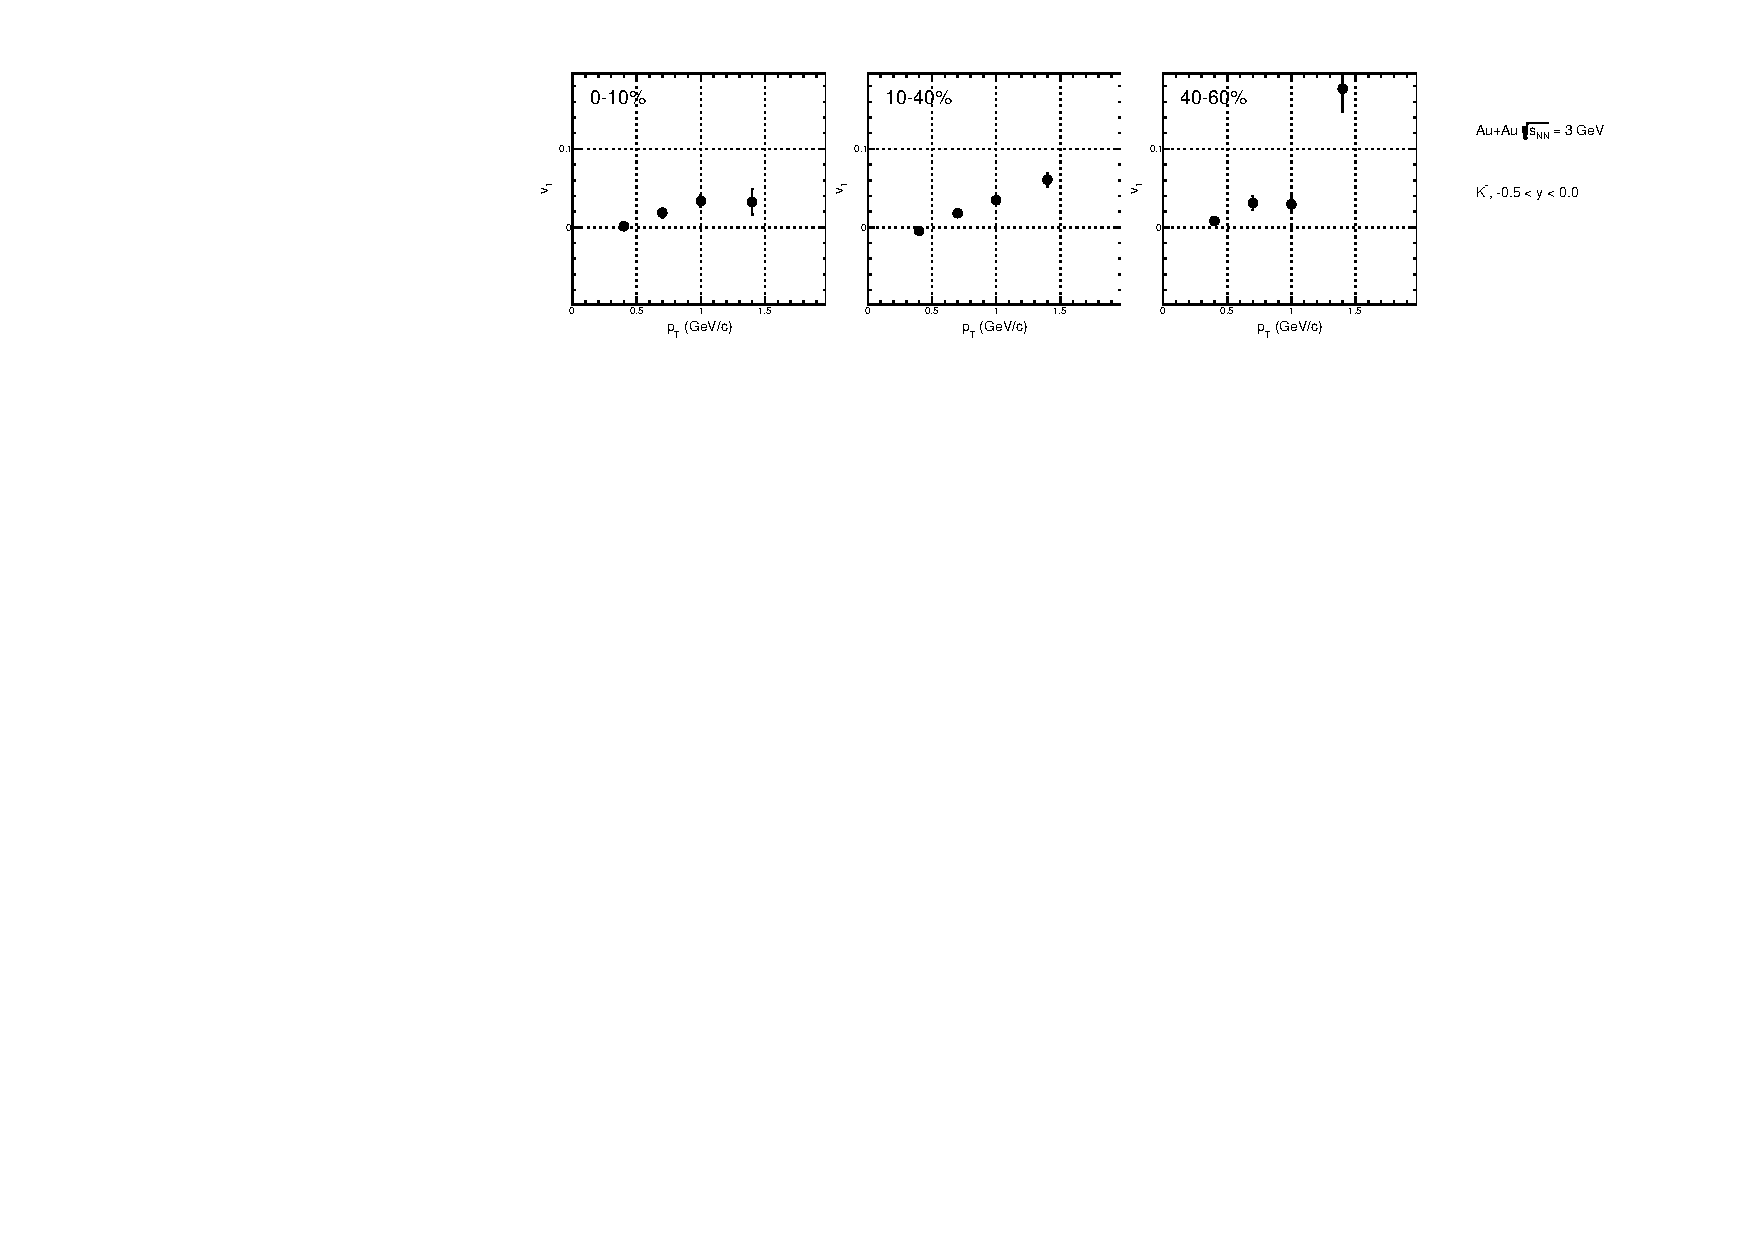
\includegraphics[scale=0.5]{chapter3/fig/v1ptpikp/kaonm_v1pt_wide_cent.pdf}
\caption{kaons' $v_{1}$ as a function of transverse momentum ($p_{T}$) in Au+Au collisions at $\sqrt{s_{NN}}$ = 3 GeV in 0-10\%, 10-40\% and 40-60\% centrality bins.}
\label{kaon_v1pt_widecent}
\end{figure}

\clearpage

\subsubsection{proton $v_{1}$ as a function of $p_{T}$ and rapidity}
In this chapter, we will show the results of proton $v_{1}$ as a function of $p_{T}$ and rapidity(y). 
Figure \ref{proton_v1y_cent} shows proton $v_{1}$ as a function of y for different centrality bins from 0-5\% to 50-60\%, The red line is fitting function \ref{fit_v1_formula}, $p_{T}$ range is [0.4, 2.0] GeV/c, which is same with STAR BES-I results. As we can see, the magnitude of proton's $v_{1}$ has centrality dependence, figure \ref{proton_dv1dy_cent} shows proton $dv_{1}/dy$ as a function of centrality. In order to make comparison to STAR BES-I results, we have these results in wider centrality bin in the figure \ref{proton_v1y_widecent}. And the $v_{1}$ slope has maximum value in the mid-central collision.


\begin{figure}[h]
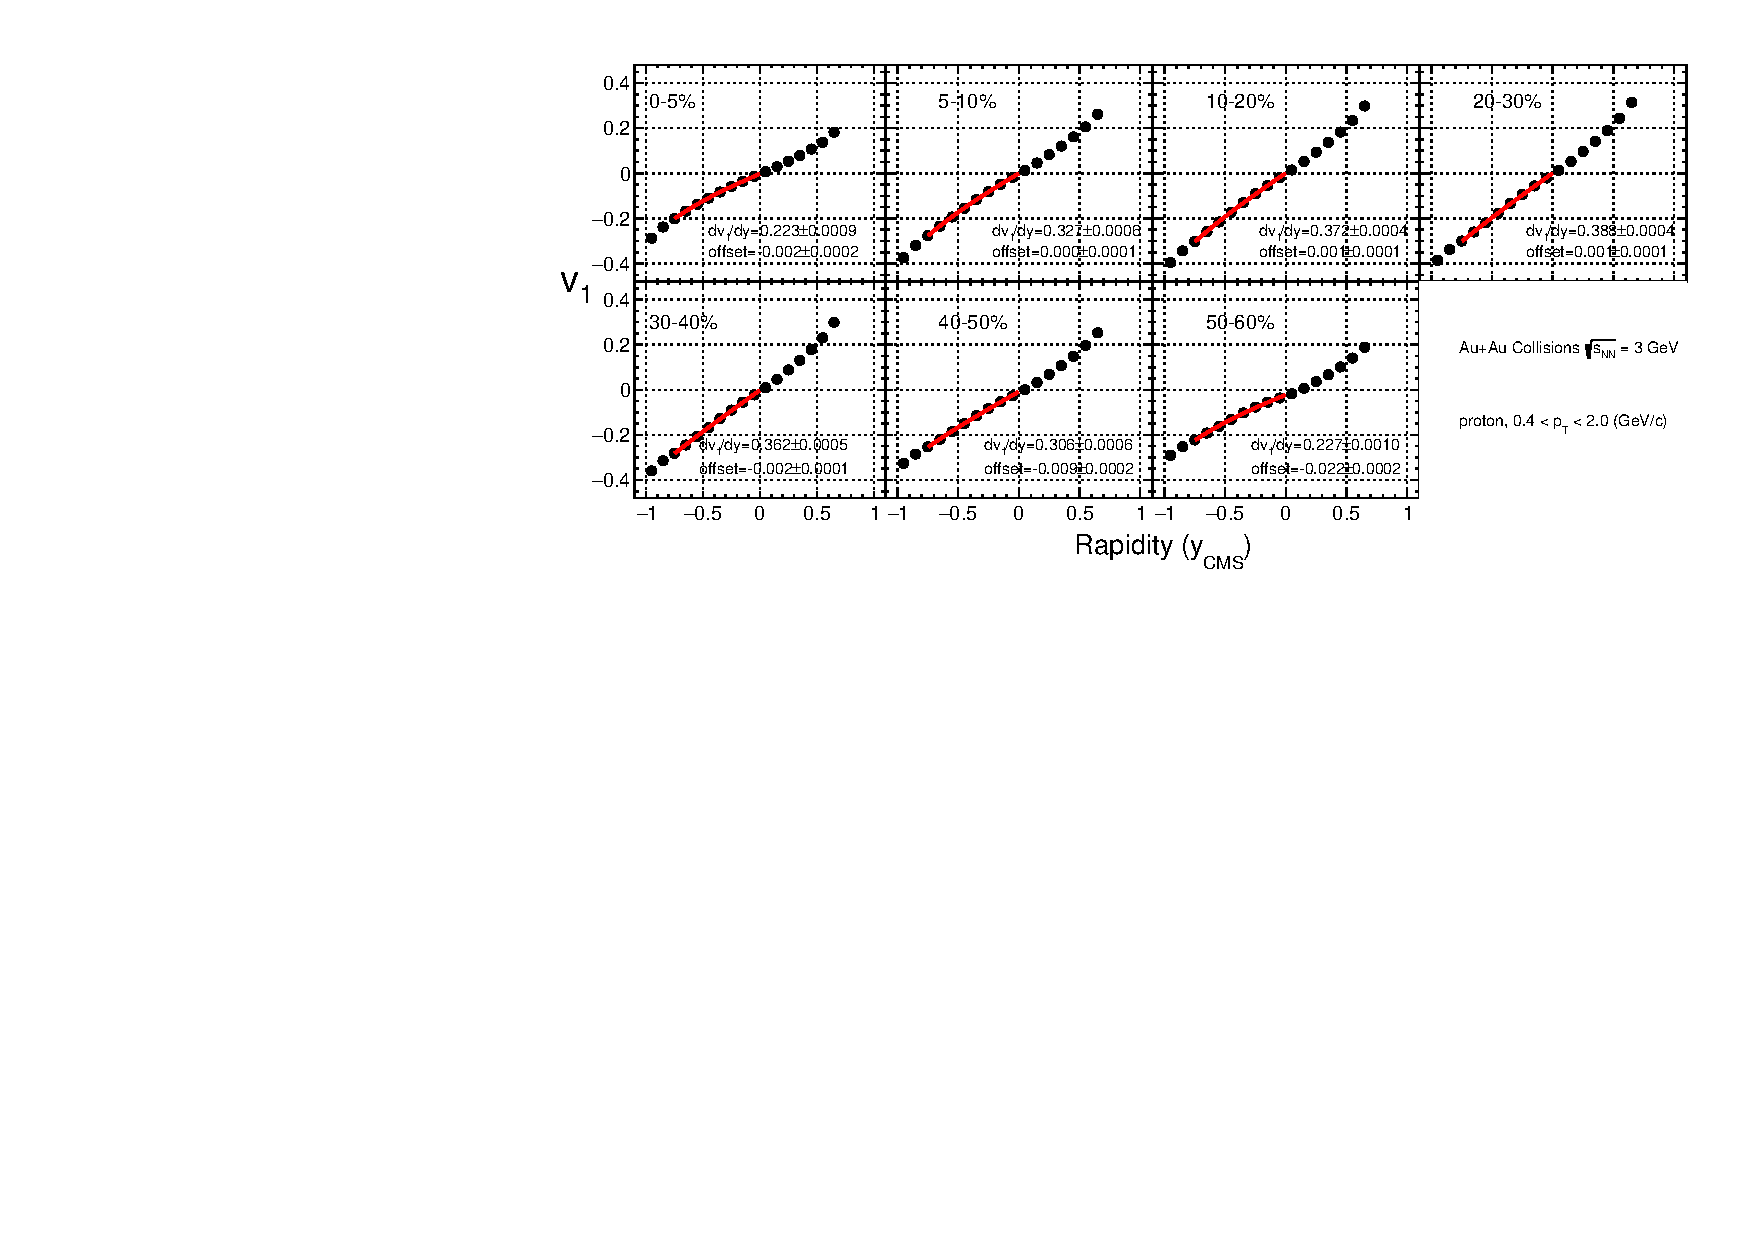
\includegraphics[scale=0.8]{chapter3/fig/v1ypikp/v1proton_cent.pdf}
\caption{\label{proton_v1y_cent} $v_{1}$ as a function of rapidity(y) in different centrality bins for proton in Au+Au collisions at $\sqrt{s_{NN}}$. The red line is fitting function.}
\end{figure}

\begin{figure}[h]
\centering
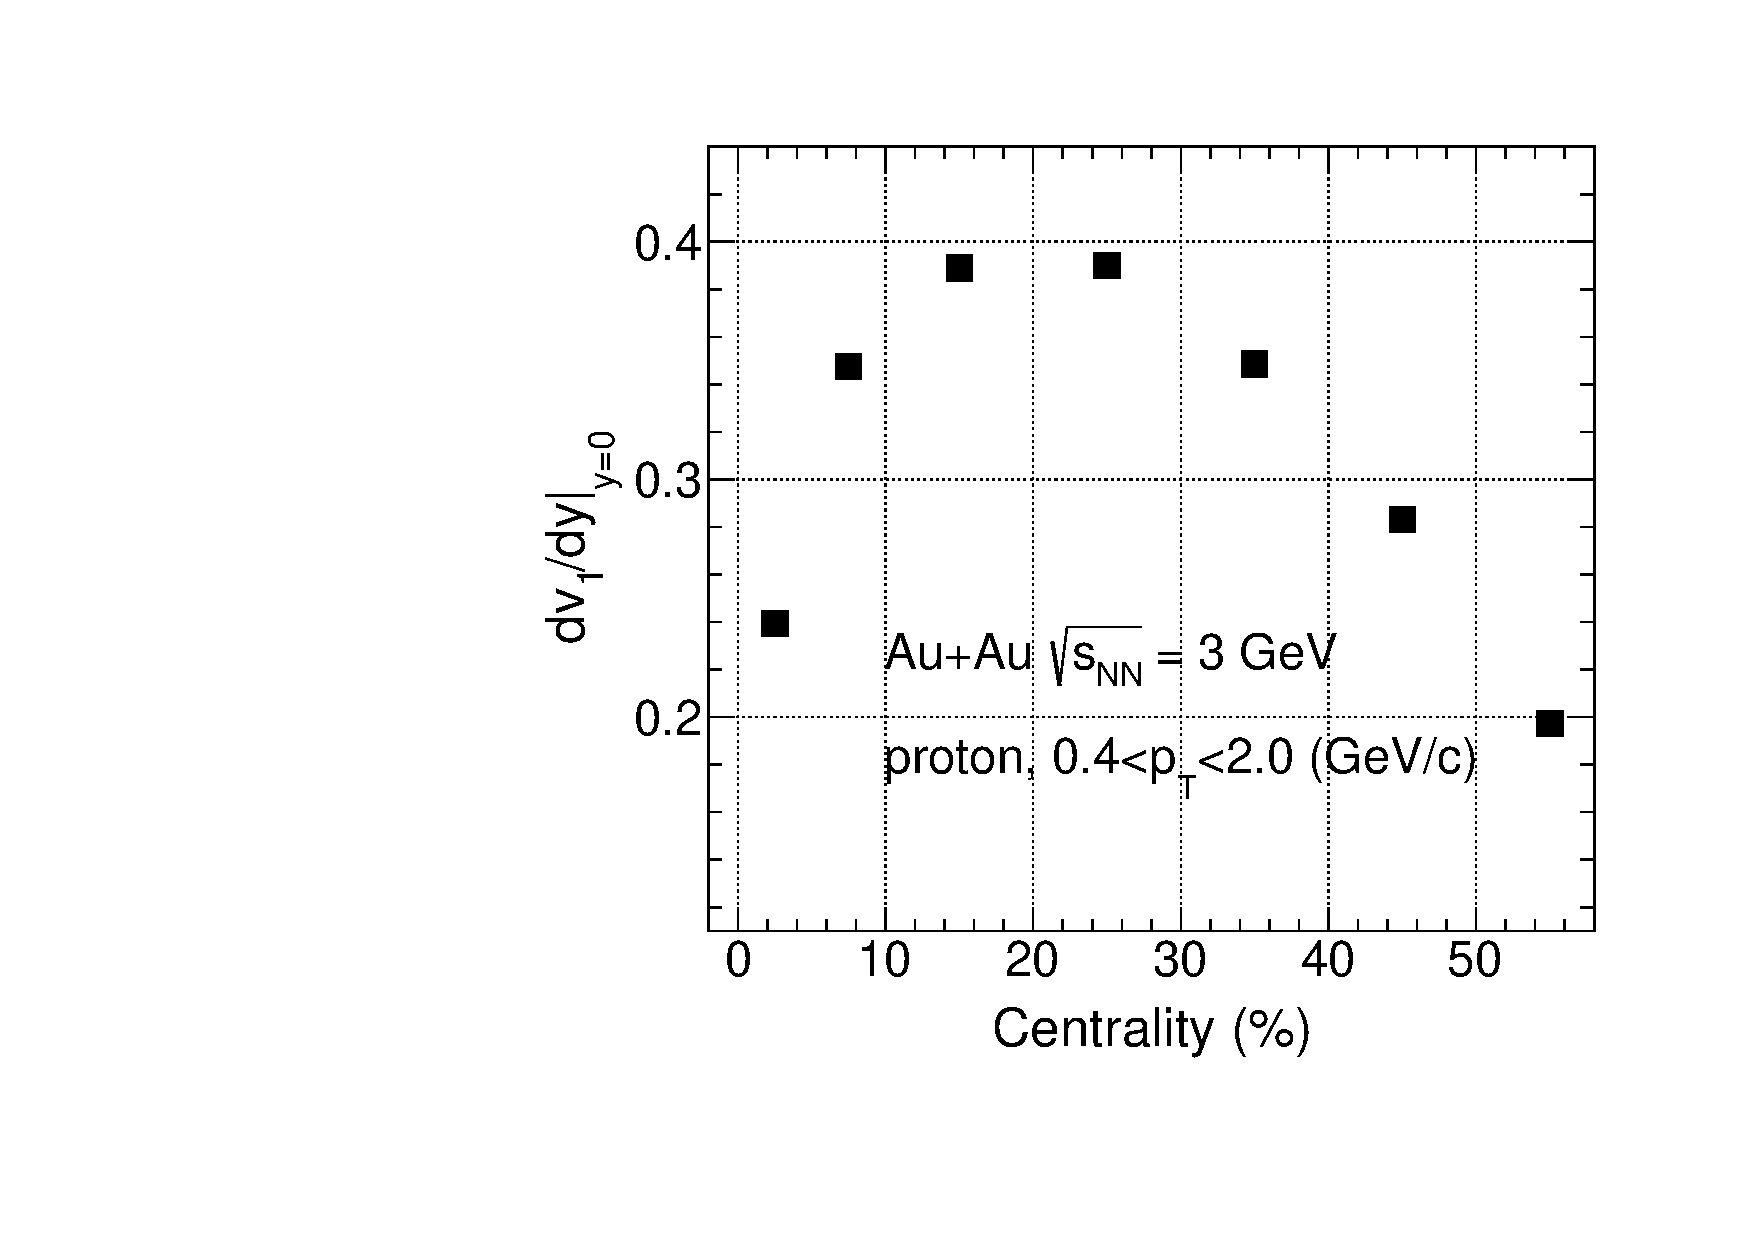
\includegraphics[scale=0.5]{chapter3/fig/v1ypikp/dv1dy_proton.pdf}
\caption{\label{kaon_dv1dy_cent} protons' $v_{1}$ slope $dv_{1}/dy$ as a function of centrality in Au+Au collisions $\sqrt{s_{NN}}$ = 3GeV.}
\end{figure}

\begin{figure}[h]
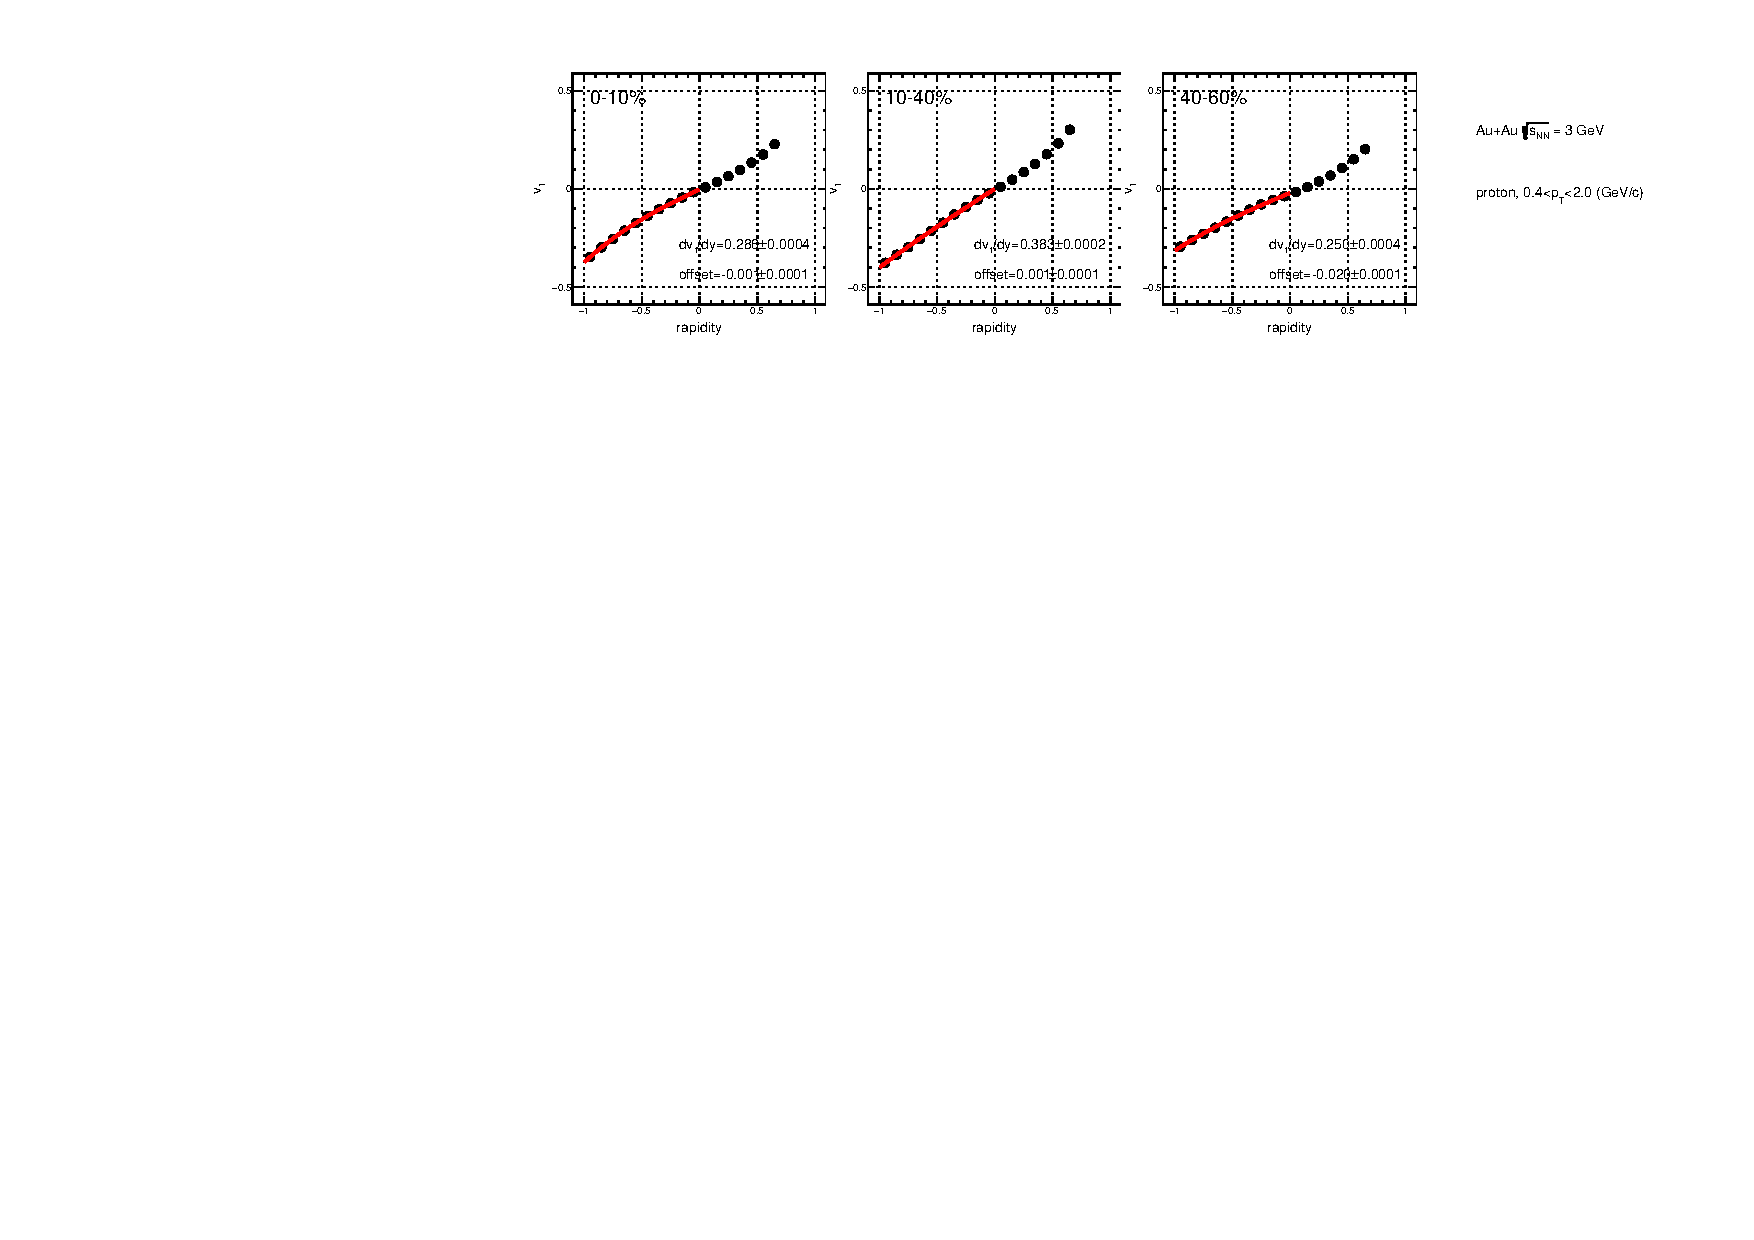
\includegraphics[scale=0.8]{chapter3/fig/v1ypikp/protonp_v1y_wide_cent.pdf}
\caption{\label{proton_v1y_widecent} protons' $v_{1}$ as a function of rapidity(y) in Au+Au collision at $\sqrt{s_{NN}}$=3GeV in 0-10\%, 10-40\% and 40-60\% bins.}
\end{figure}

\clearpage

We also study the $p_{T}$ dependence of protons' $v_{1}$ in the mid-rapidity region (-0.5$<$y$<$0) in different centrality bins in the figure \ref{proton_v1pt_cent}. As we can see, protons $v_{1}$ is increasing with $p_{T}$ increasing. Figure \ref{proton_v1pt_widecent} also shows the results in the wider centrality bins. Since we do see the clear $p_{T}$ and rapidity dependence for proton $v_{1}$ and we have fruitful statistics for proton at 3 GeV, we would like to do the 2D scan for proton $v_{1}$, 1: we scan $p_{T}$ bins to plot $v_{1}$ as a function of rapidity, 2: we scan rapidity bins to plot $v_{1}$ as a function of $p_{T}$. As we can see in the figure \ref{v1_2dscan_proton}.

\begin{figure}[h]
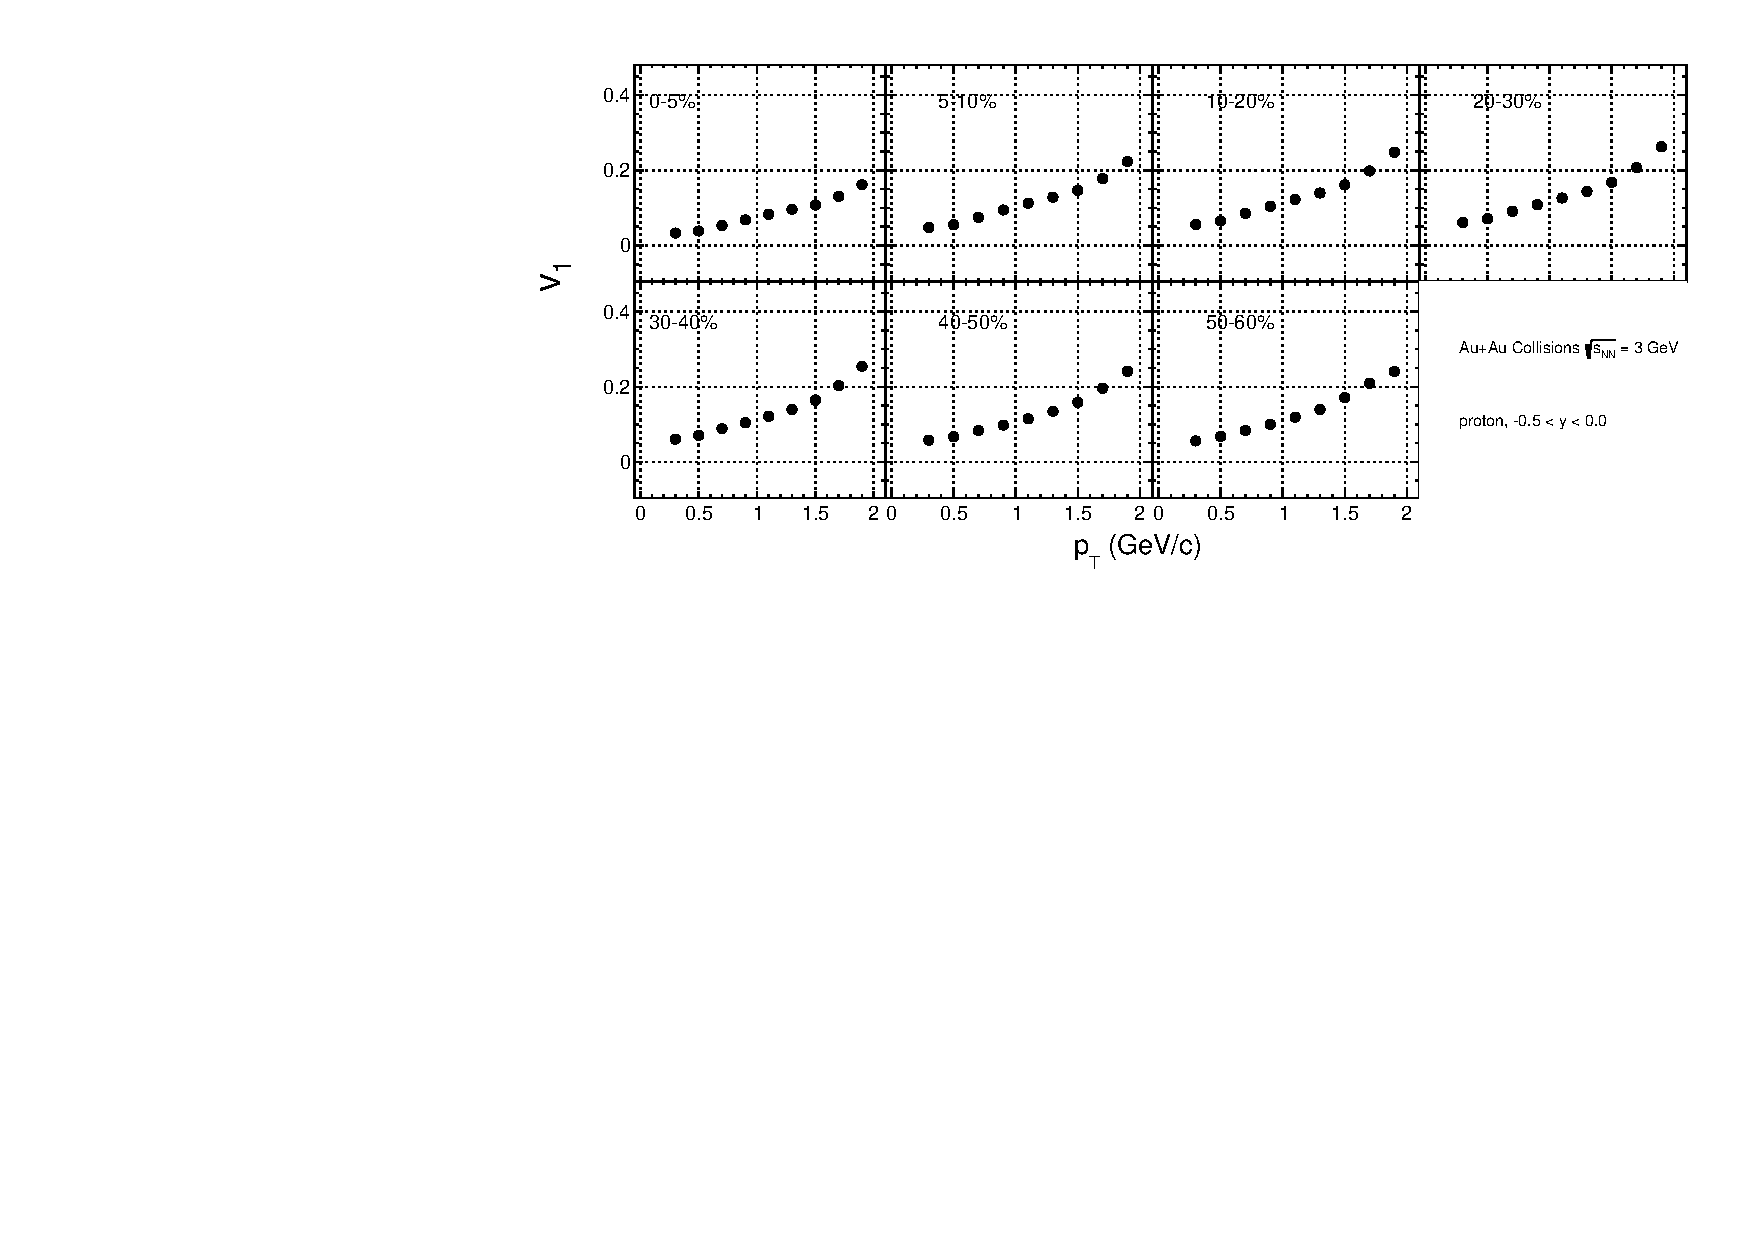
\includegraphics[scale=0.7]{chapter3/fig/v1ptpikp/v1pt_cent_proton.pdf}
\caption{protons' $v_{1}$ as a function of transverse momentum ($p_{T}$) in Au+Au collisions at $\sqrt{s_{NN}}$ = 3 GeV.}
\label{proton_v1pt_cent}
\end{figure}

\begin{figure}[h]
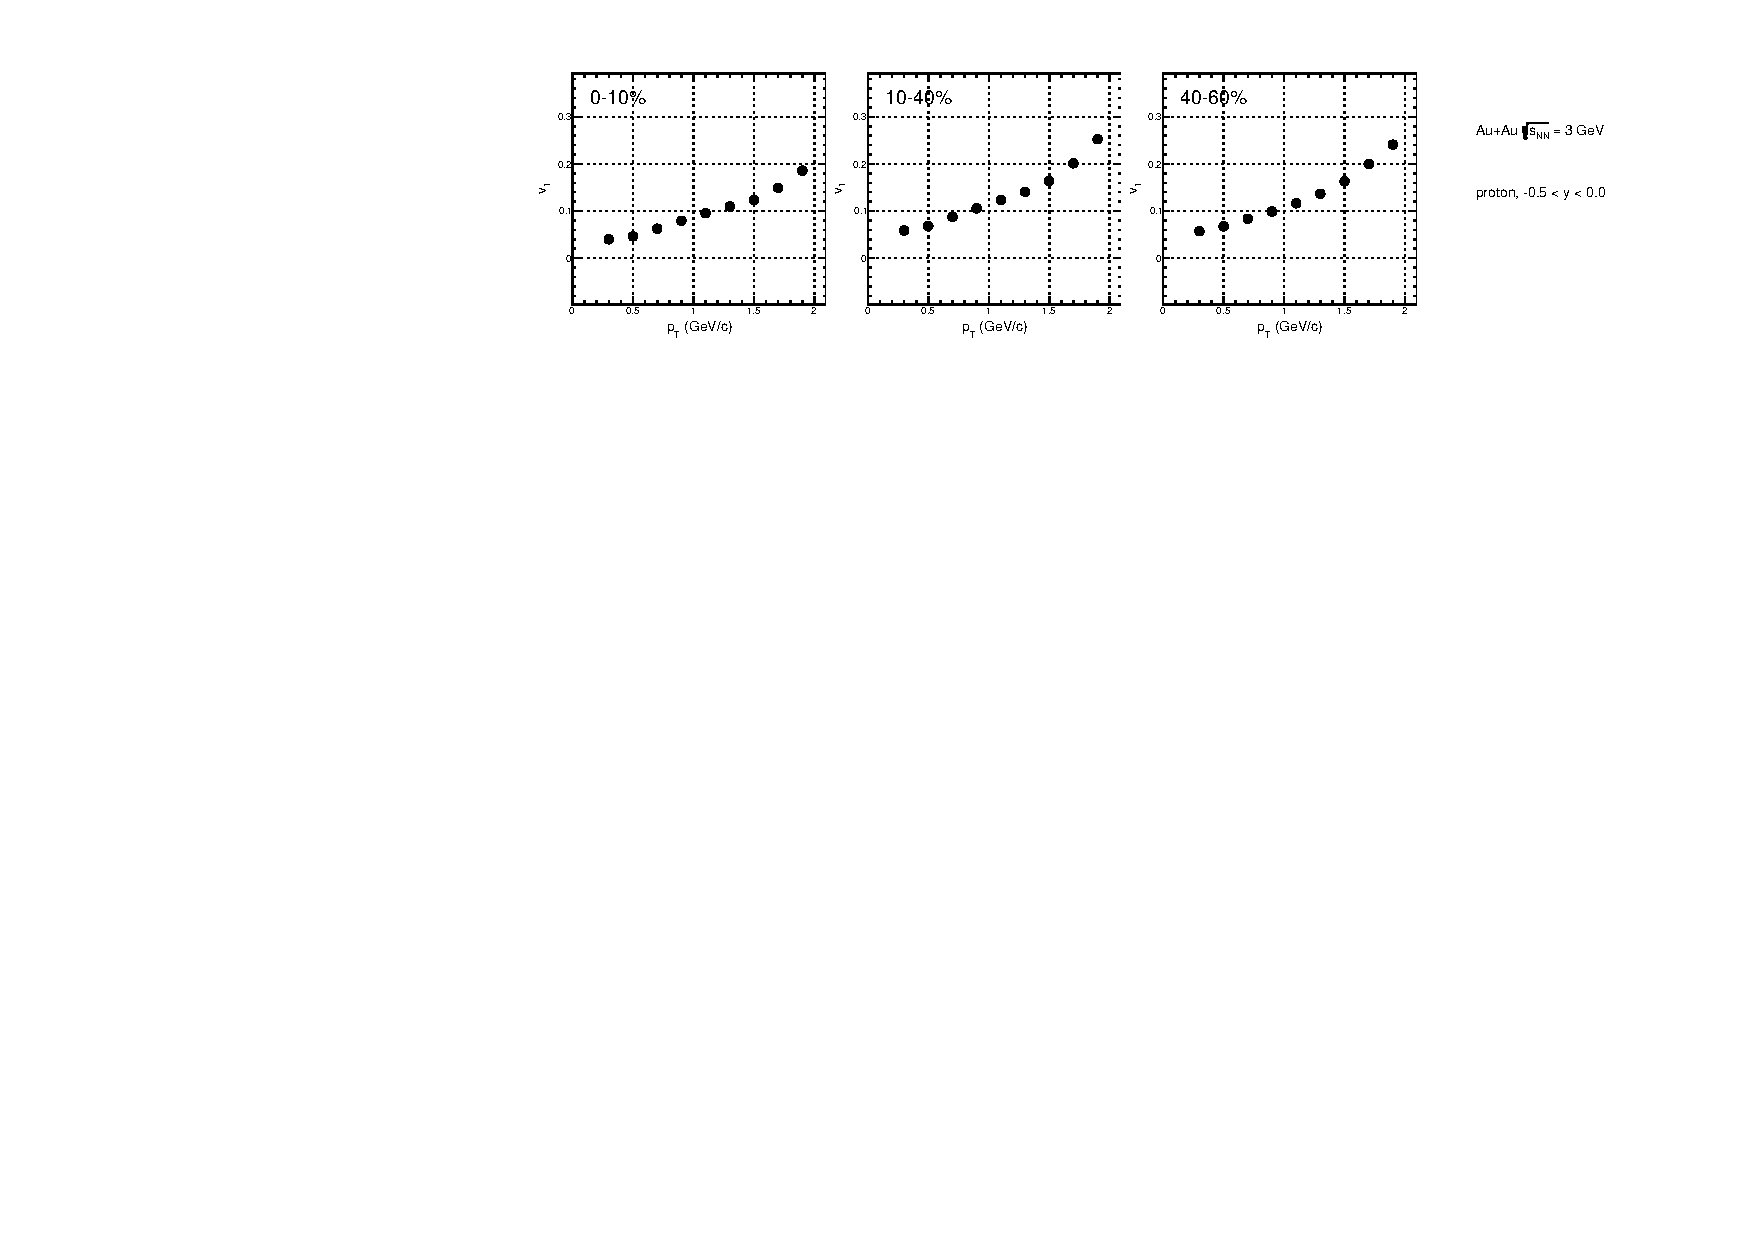
\includegraphics[scale=0.7]{chapter3/fig/v1ptpikp/protonp_v1pt_wide_cent.pdf}
\caption{protons' $v_{1}$ as a function of transverse momentum ($p_{T}$) in Au+Au collisions at $\sqrt{s_{NN}}$ = 3 GeV in 0-10\%, 10-40\% and 40-60\% centrality bins.}
\label{proton_v1pt_widecent}
\end{figure}

\begin{figure}[h]
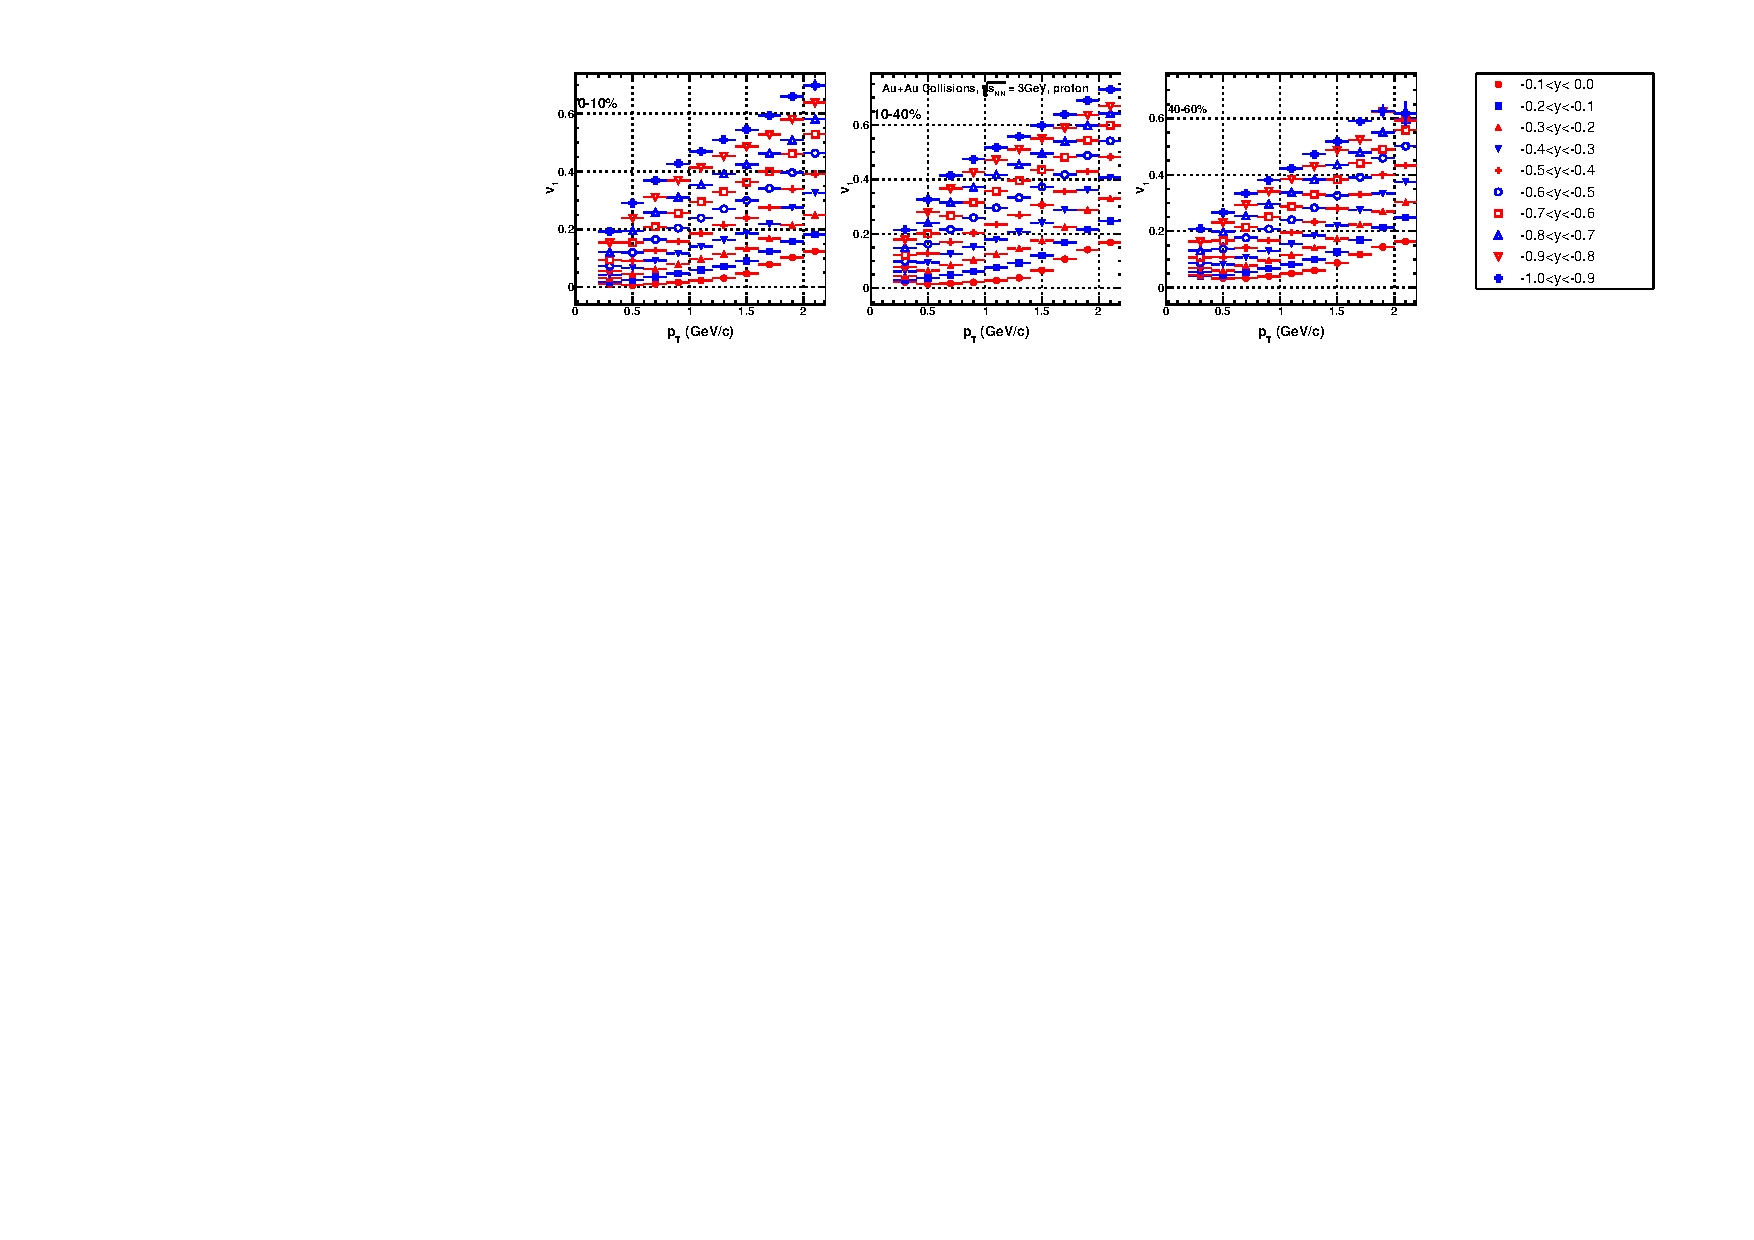
\includegraphics[scale=0.7]{chapter3/fig/2dscan/protonp_y_scan_v1pt.pdf}
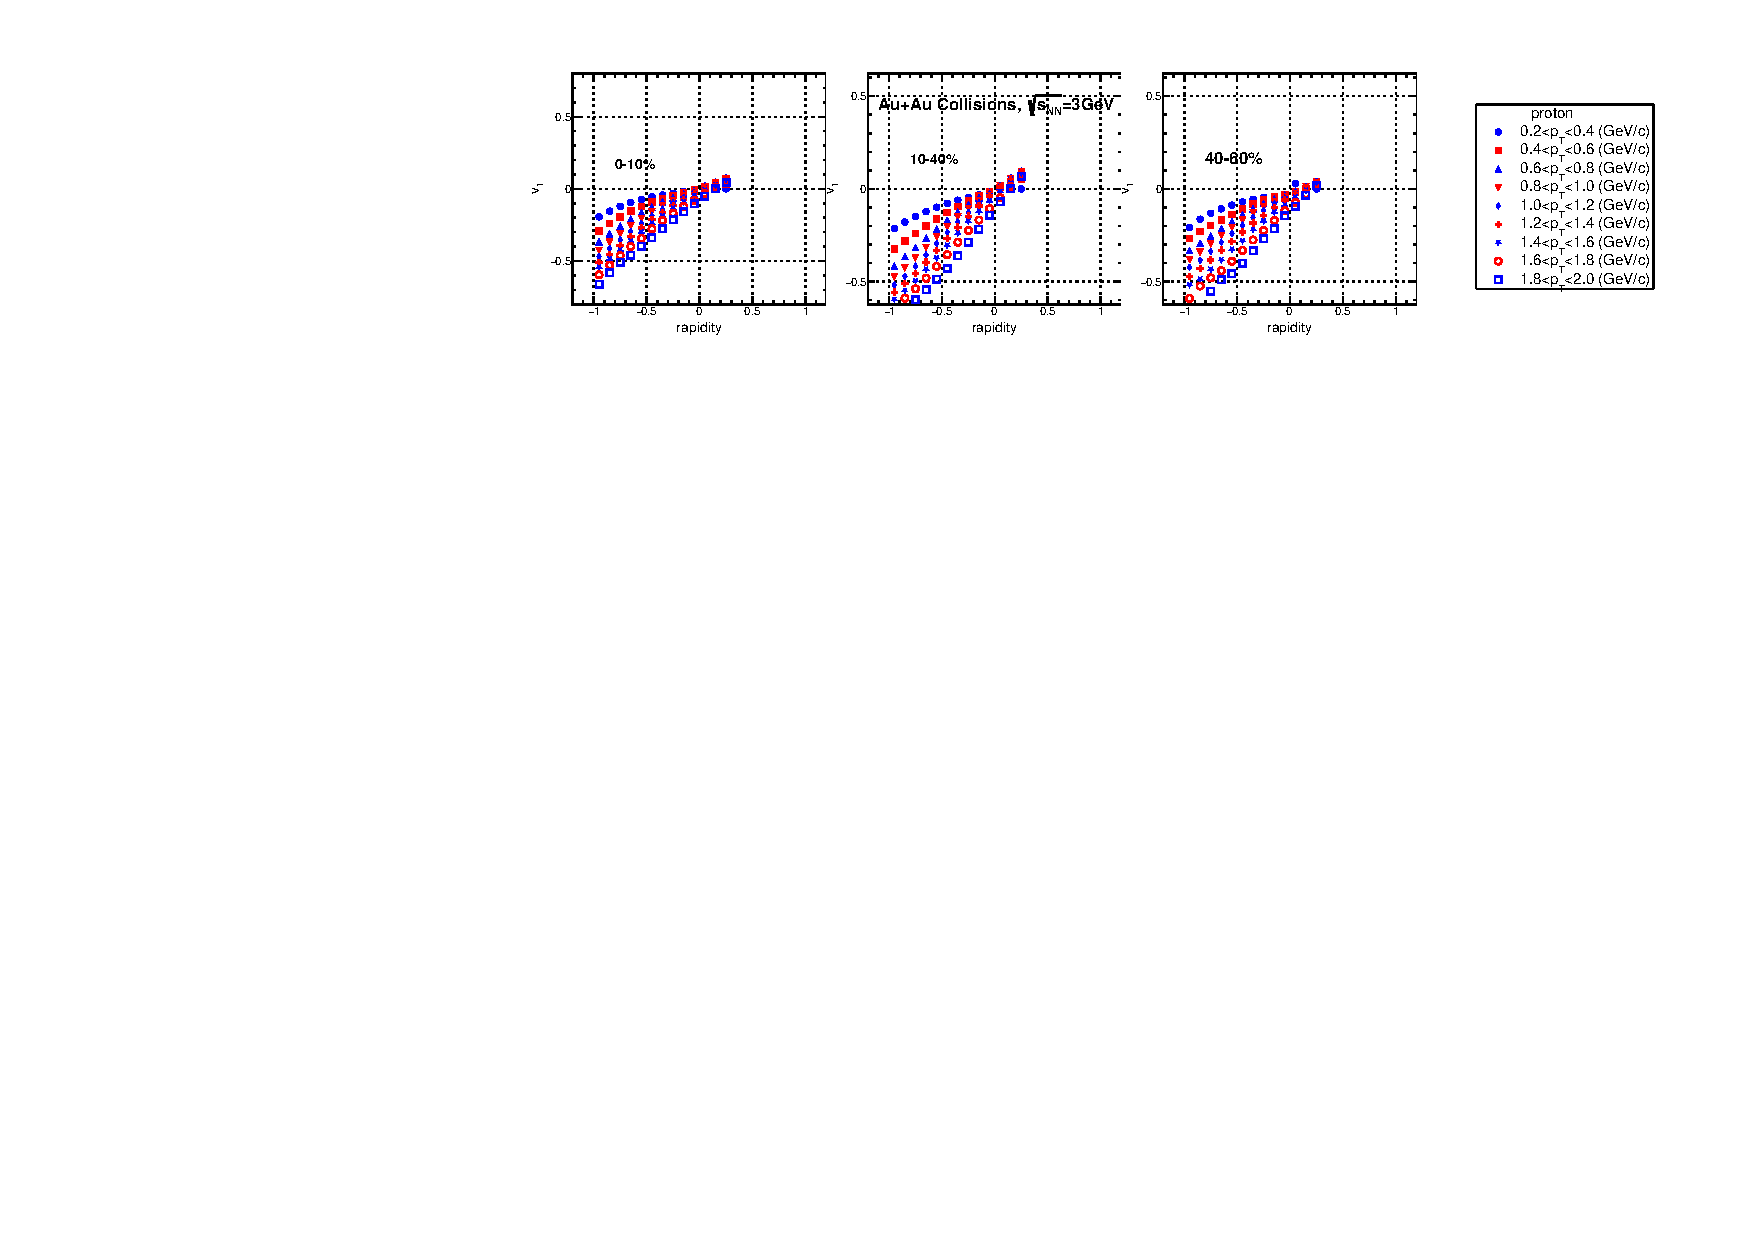
\includegraphics[scale=0.7]{chapter3/fig/2dscan/protonp_pt_scan_v1y.pdf}
\caption{protons' $v_{1}$ as a function of $p_{T}$ in fine rapidity bins and as a function of rapidity in fine $p_{T}$ bins in 0-10\%, 10-40\% and 40-60\% at $\sqrt{s_{NN}}$ 3 GeV.}
\label{v1_2dscan_proton}
\end{figure}


\clearpage
\subsection{$v_{2}$ results for $\pi, K, p$}
In this chapter, we will show the $v_{2}$ as a function of $p_{T}$ and rapidity(y) in fine centrality bins for $\pi^{\pm}, K^{\pm}$ and proton. It is expected to have a negative $v_{2}$ value at mid-rapidity region based on world data due to the "squeeze-out" effect when the center of mass energy is below 4 GeV. This is because at such low energy, the passage time of projectile and target spectators is comparable or larger than the expansion time QGP mediums, thus the spectators will shadow or squeeze out the medium expansion in the impact parameter direction, which will results in the out-of plane $v_{2}$, the negative $v_{2}$ value.

\subsubsection{pions $v_{2}$ as a function of $p_{T}$ and rapidity}
In this chapter, we will show the results of pions' $v_{2}$ as a function of $p_{T}$ and rapidity(y).
Figure \ref{pion_v2y_cent} shows pion $v_{2}$ as a function of y for different centrality bins from 0-5\% to 50-60\%. The $p_{T}$ range is [0.2, 1.6] GeV/c. As we can see, we have observed the negative pion $v_{2}$ value at mid-rapidity region, and it has weak rapidity dependence for both $\pi^{+}$ and $\pi^{-}$. Which we do see the difference between $\pi^{+}$ and $\pi^{-}$ $v_{2}$, $\pi^{-}$ $v_{2}$ is a little larger than $\pi^{+}$ $v_{2}$. In the BES-I flow results, we also see the difference between $\pi^{+}$ and $\pi^{-}$ $v_{2}$, which has been interpreted by the isospin effect or mean-filed potential effect. Figure \ref{pion_v2y_widecent} shows the pions' $v_{2}$ vs. y in wider centrality bin.

\begin{figure}[h]
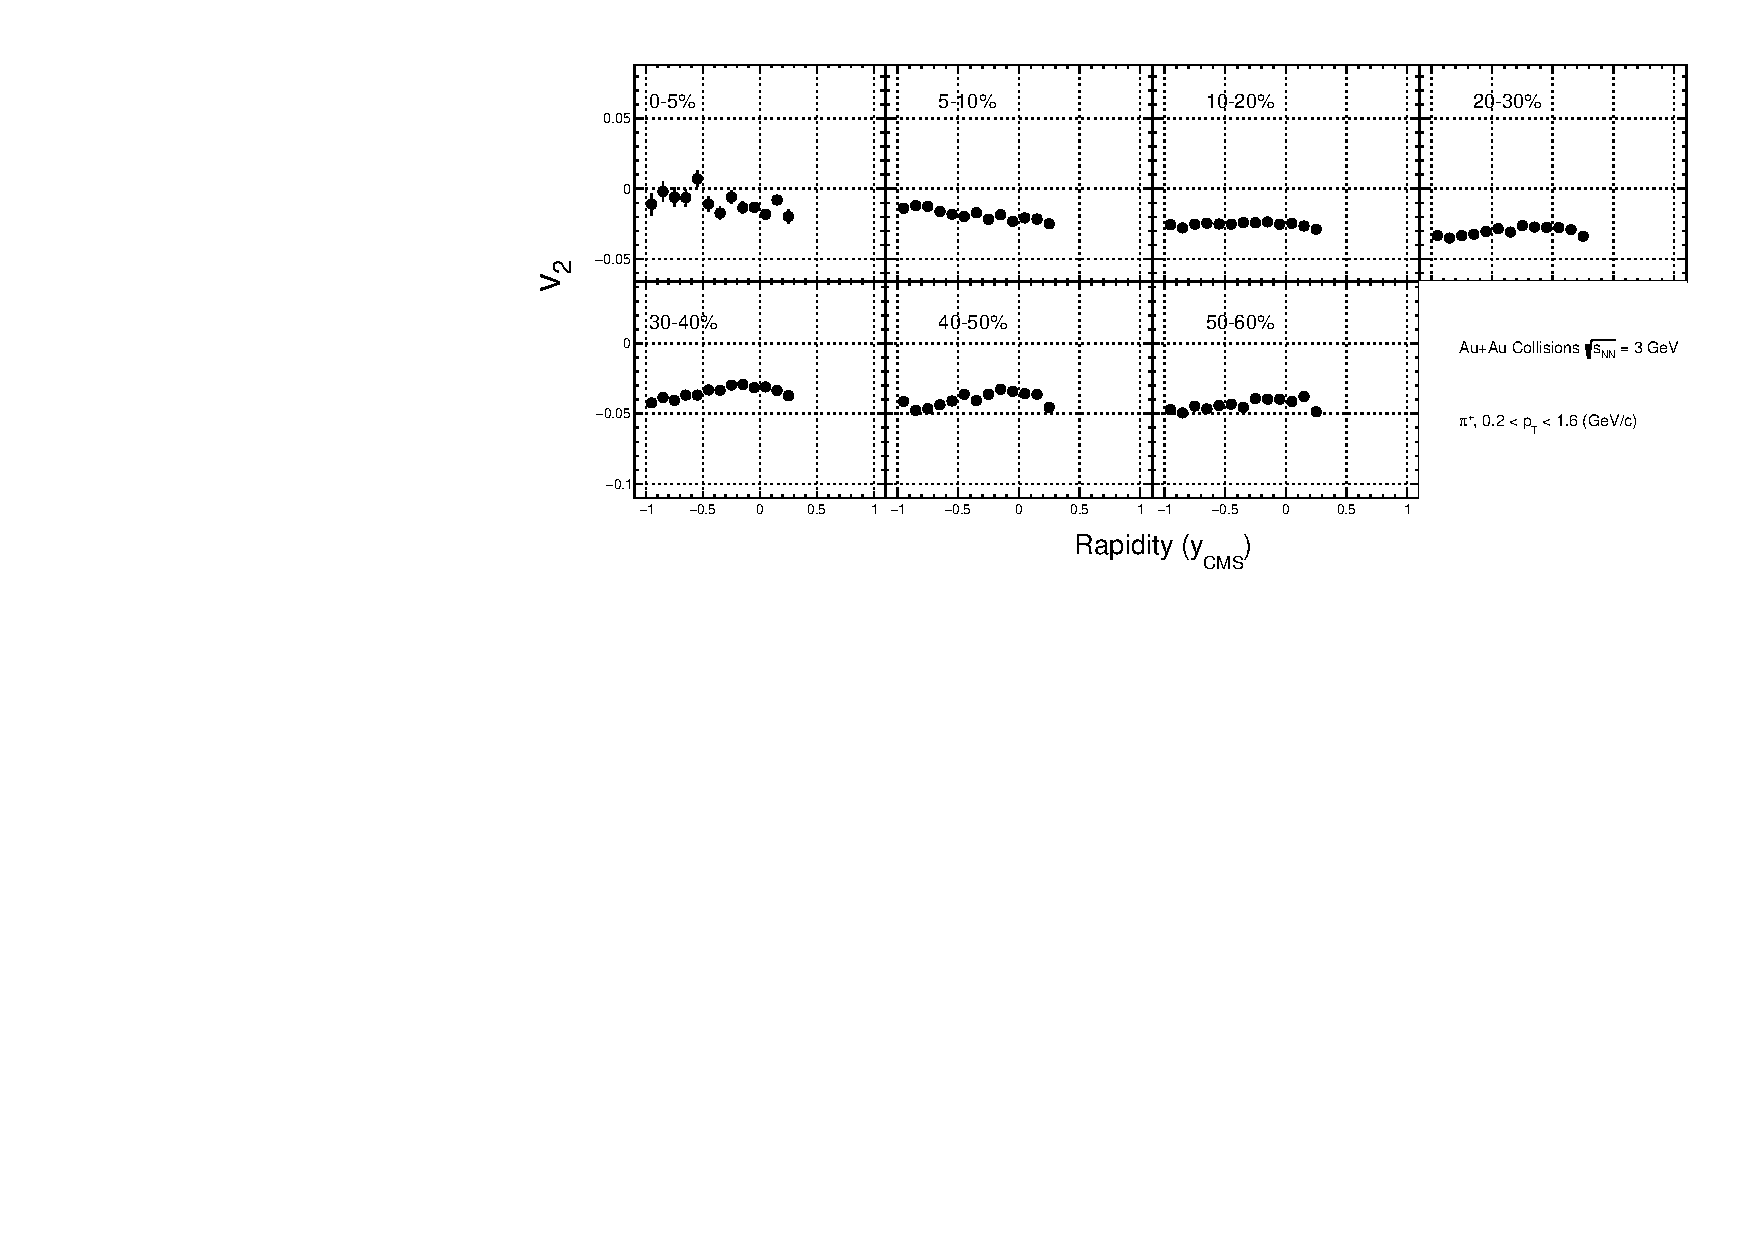
\includegraphics[scale=0.4]{chapter3/fig/v2ypikp/v2y_cent_pionp.pdf}
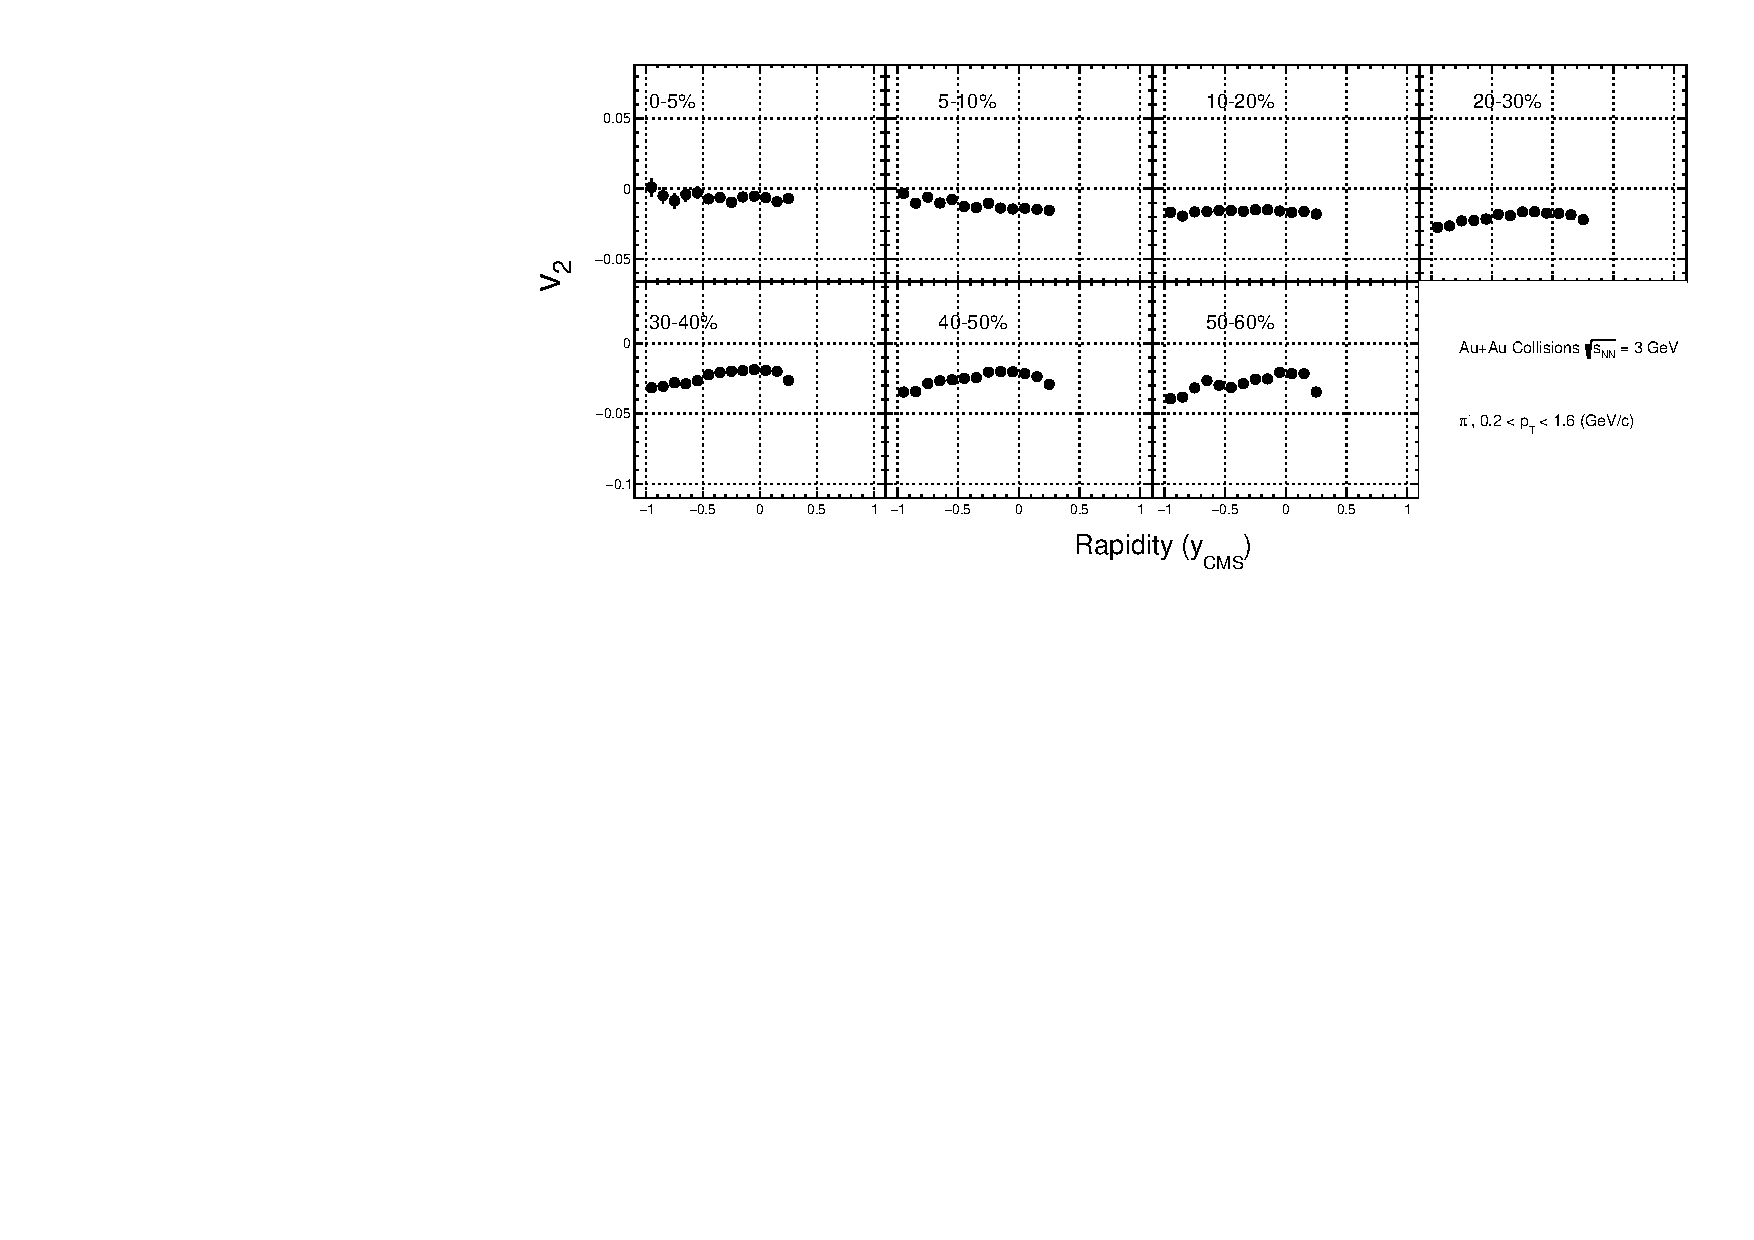
\includegraphics[scale=0.4]{chapter3/fig/v2ypikp/v2y_cent_pionm.pdf}
\caption{\label{pion_v2y_cent} $v_{2}$ as a function of rapidity(y) in different centrality bins for $\pi^{+}$ and $\pi^{-}$ in Au+Au collisions at $\sqrt{s_{NN}}$ = 3 GeV.}
\end{figure}

\begin{figure}[h]
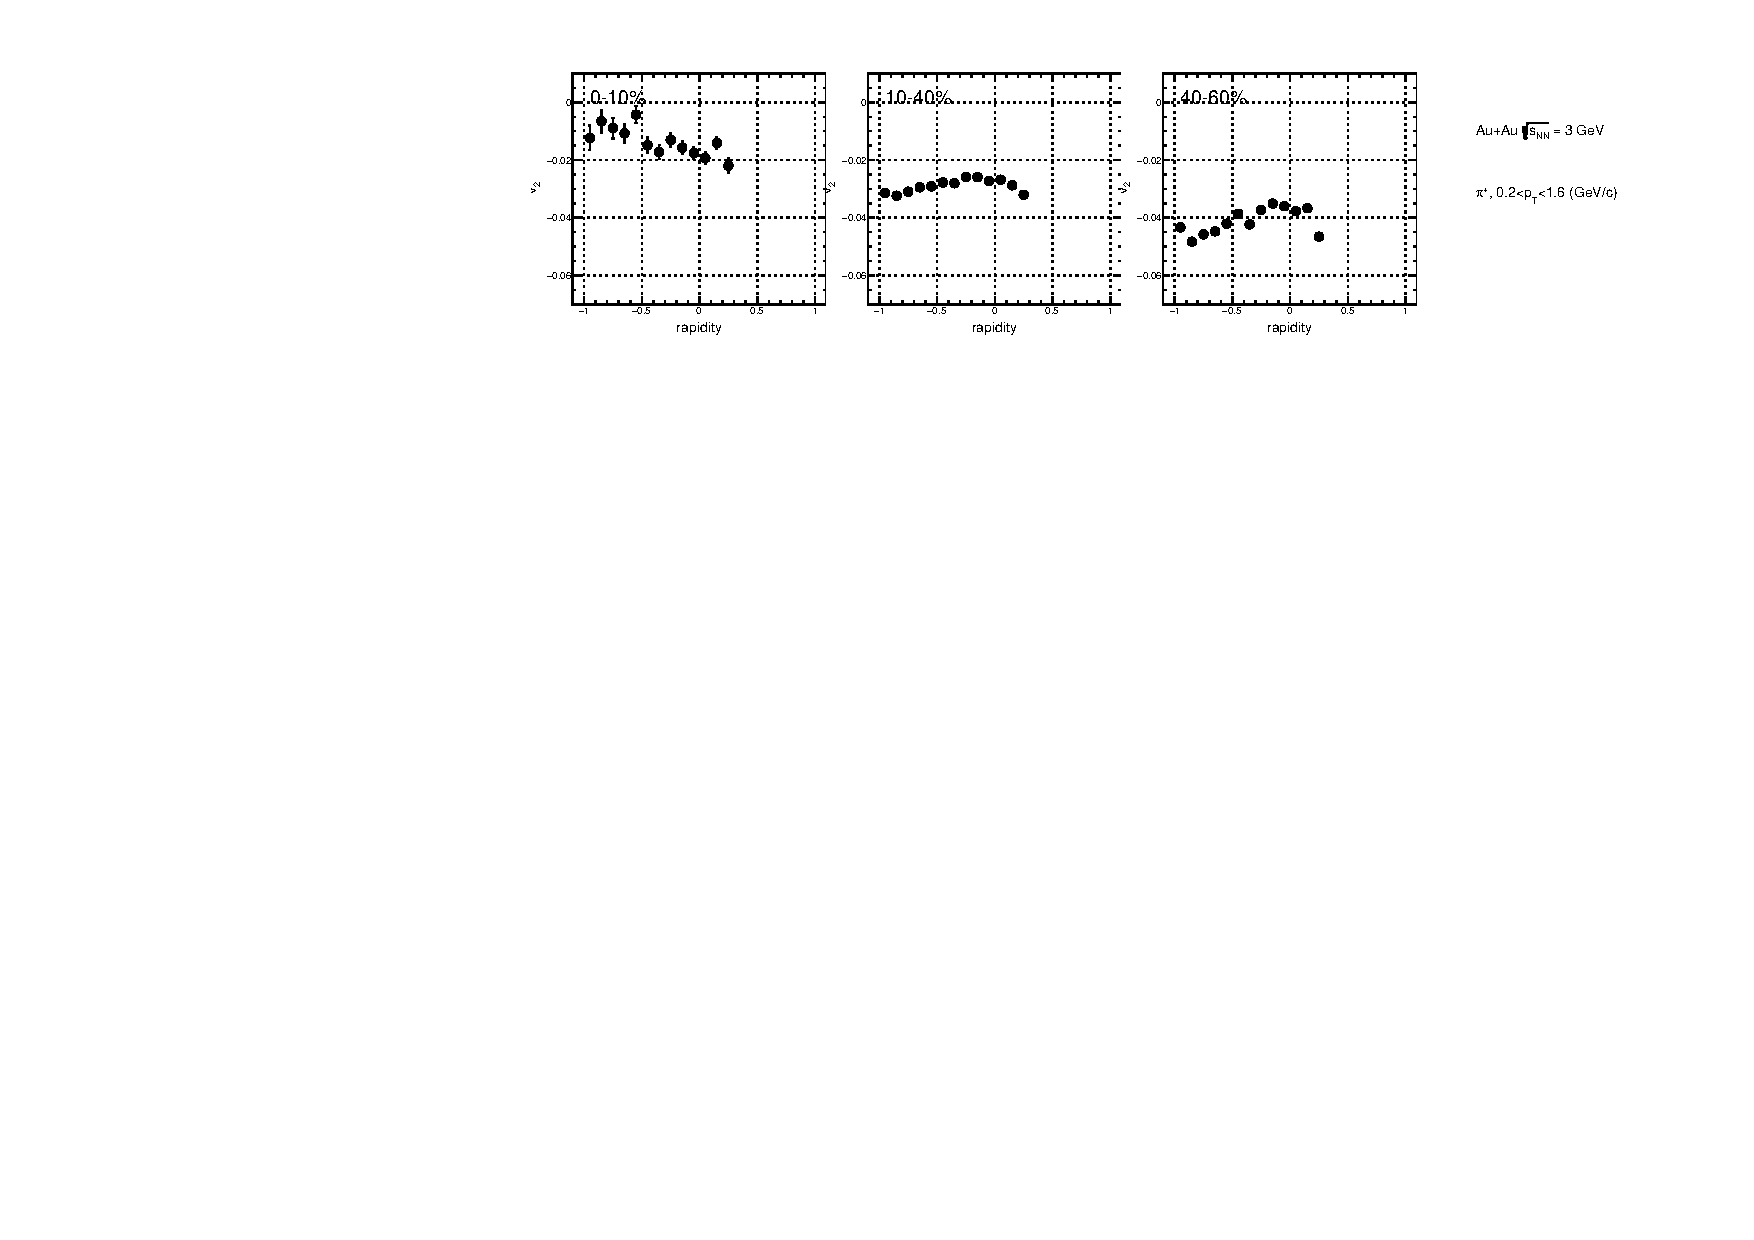
\includegraphics[scale=0.6]{chapter3/fig/v2ypikp/pionp_v2y_wide_cent.pdf}
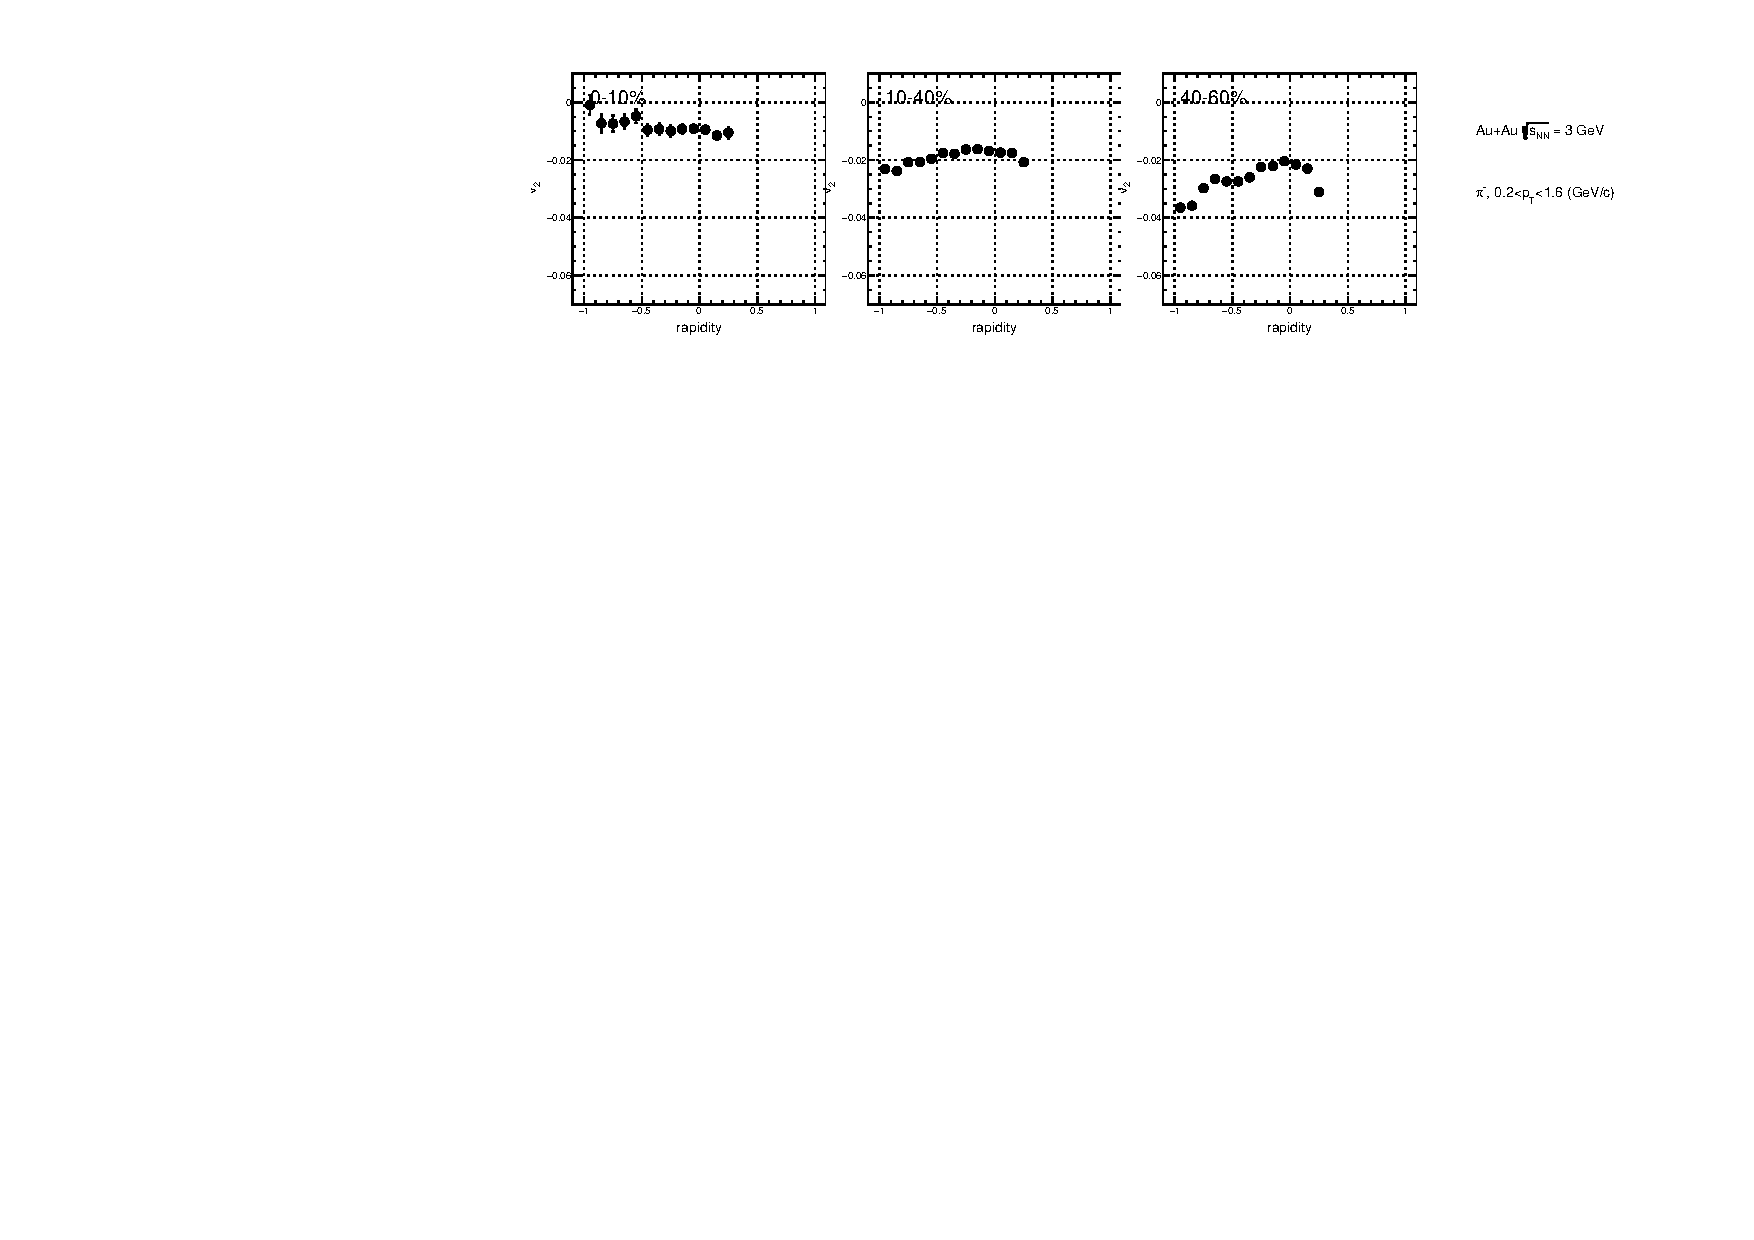
\includegraphics[scale=0.6]{chapter3/fig/v2ypikp/pionm_v2y_wide_cent.pdf}
\caption{\label{pion_v2y_widecent} $v_{2}$ as a function of rapidity(y) in different centrality bins for $\pi^{+}$ and $\pi^{-}$ in Au+Au collisions at $\sqrt{s_{NN}}$ = 3 GeV in 0-10\%, 10-40\%, 40-60\% centrality bins.}
\end{figure}

We also study the $p_{T}$ dependence for pions' $v_{2}$ in the figure \ref{pion_v2pt_cent}, as we can see, pions' $v_{2}$ is decreasing with $p_{T}$ increasing. Figure \ref{pion_v2pt_widecent} shows these results in wider centrality bins 0-10\%, 10-40\%, 40-60\%. 


\begin{figure}[h]
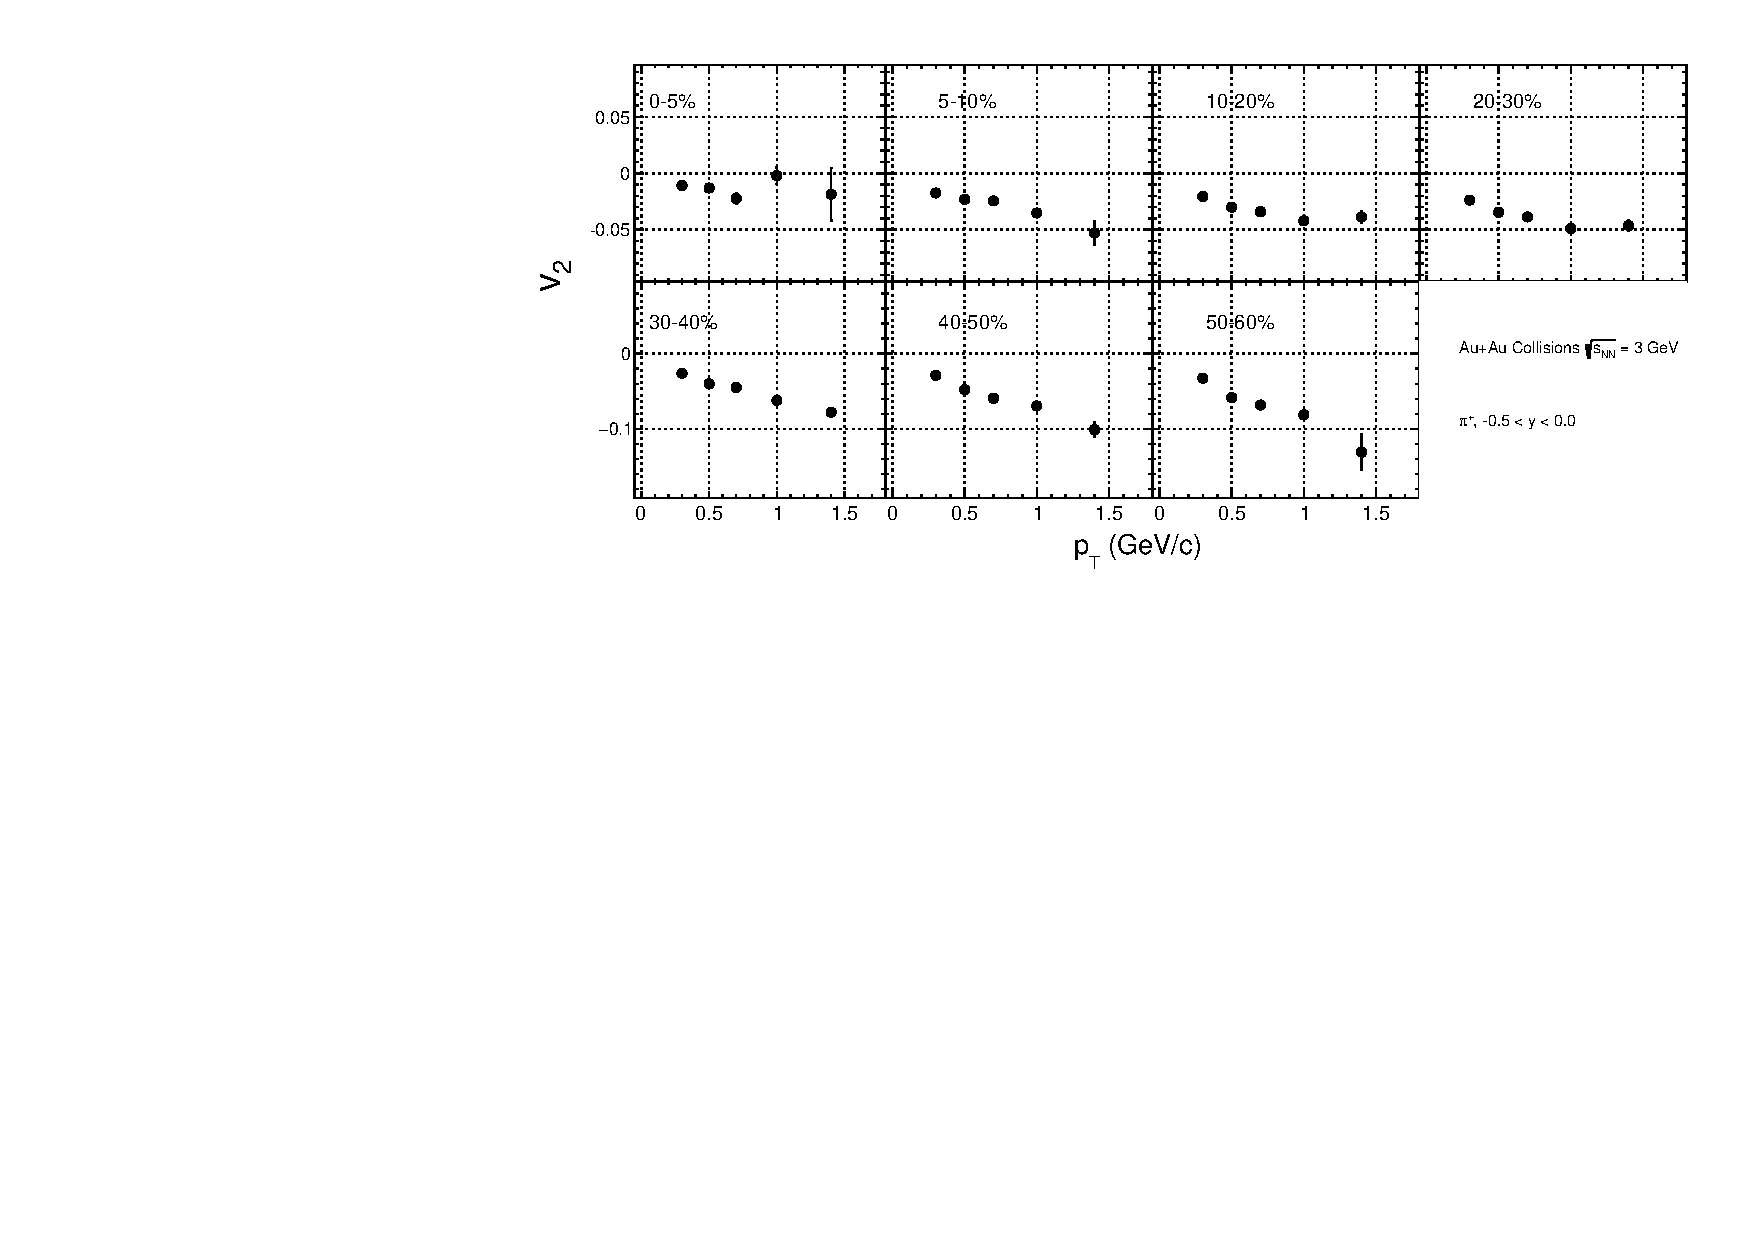
\includegraphics[scale=0.4]{chapter3/fig/v2ptpikp/v2pt_cent_pionp.pdf}
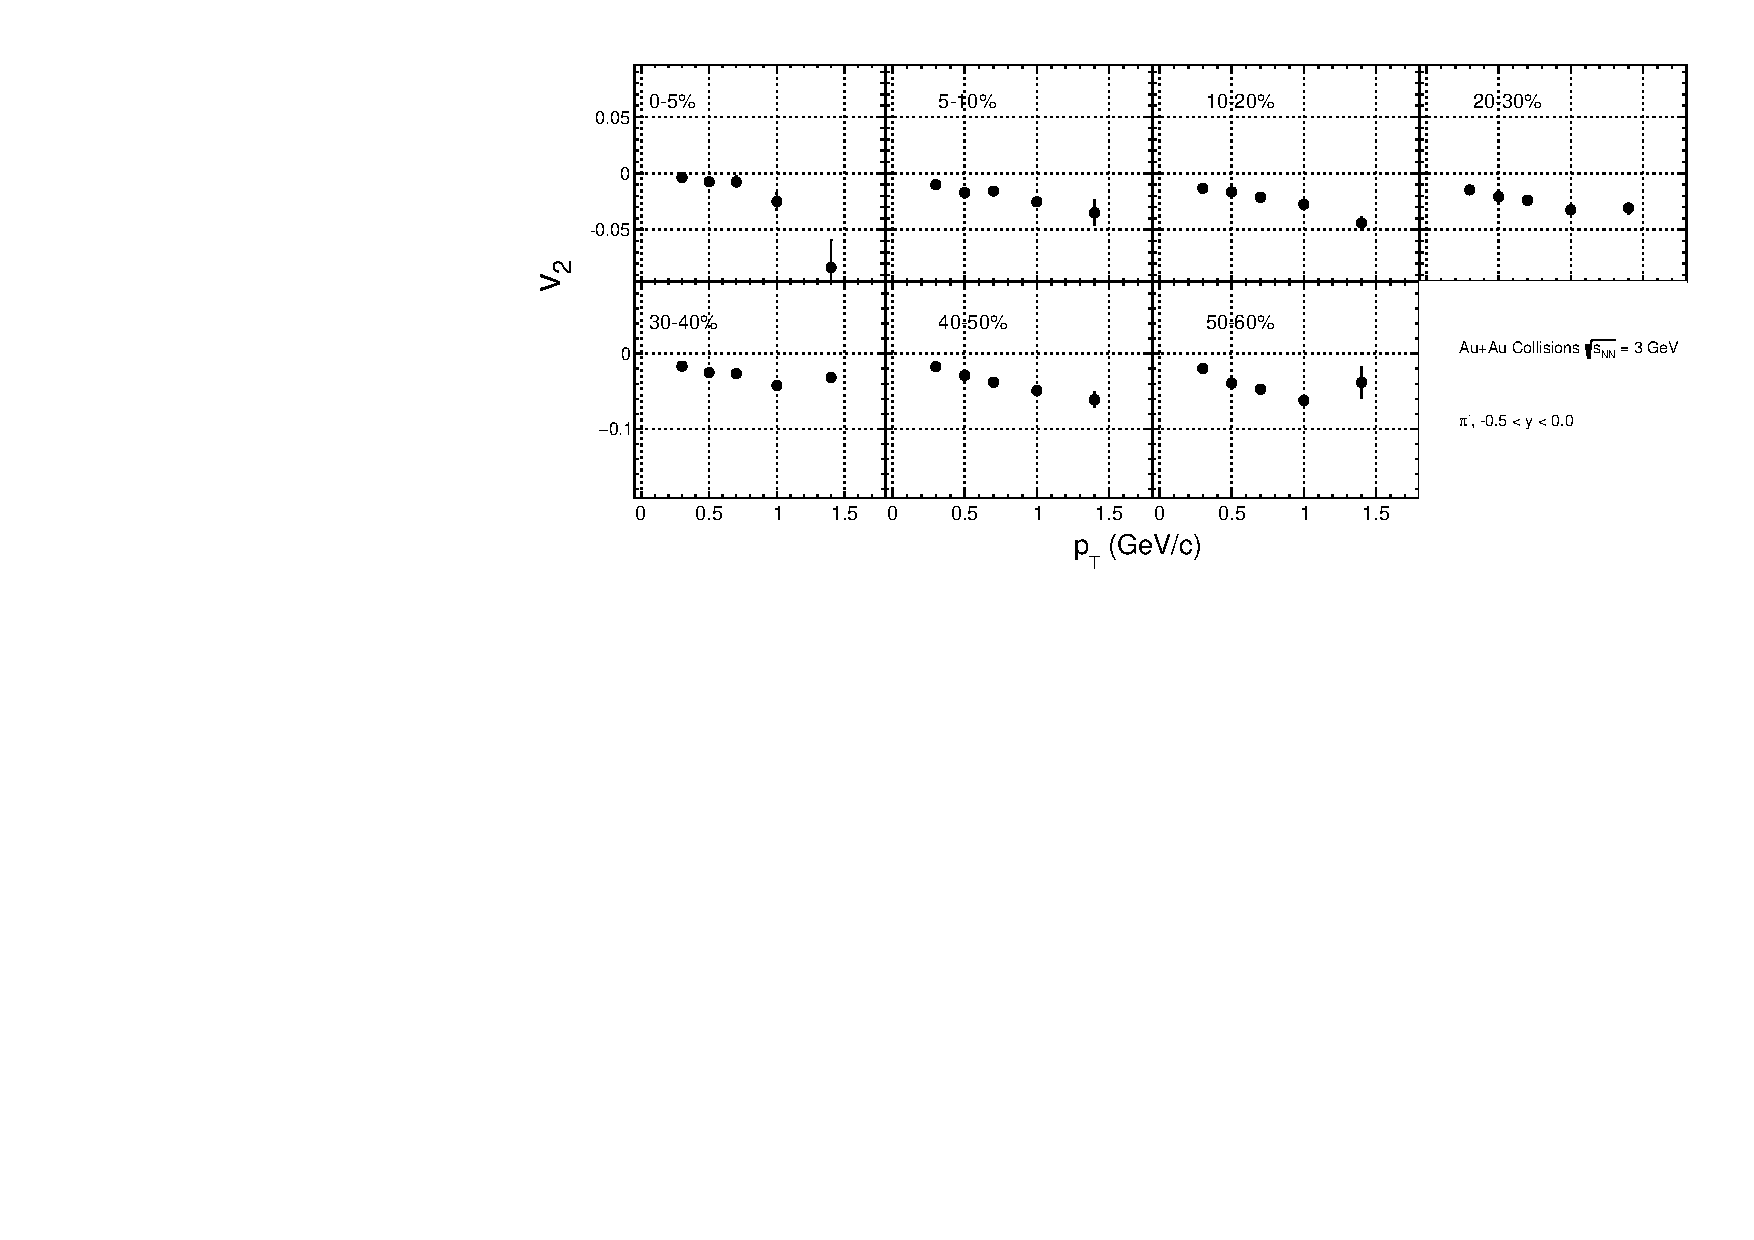
\includegraphics[scale=0.4]{chapter3/fig/v2ptpikp/v2pt_cent_pionm.pdf}
\caption{$v_{2}$ as a function of $p_{T}$ in different centrality bins for $\pi^{+}$ and $\pi^{-}$ in Au+Au collisions at $\sqrt{s_{NN}}$ = 3 GeV.}
\label{pion_v2pt_cent}
\end{figure}

\begin{figure}[h]
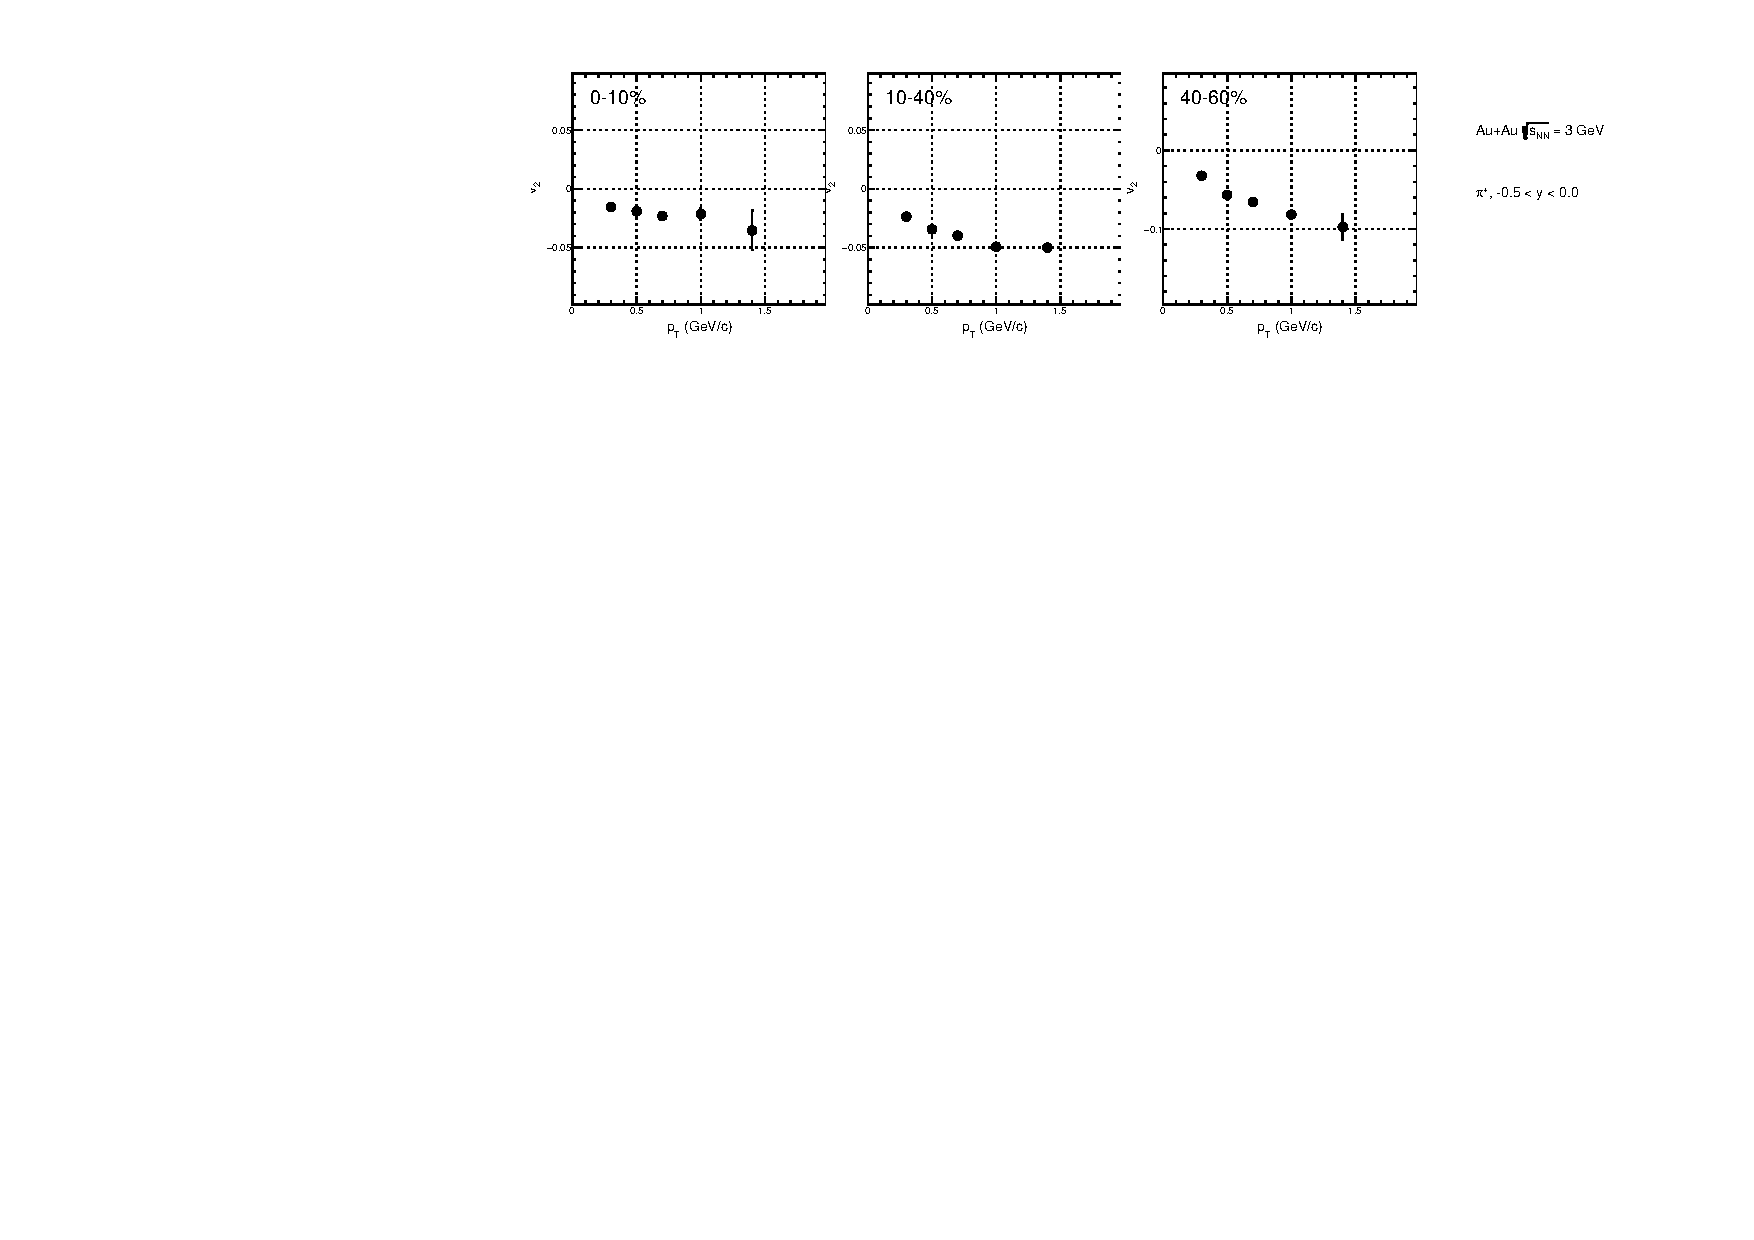
\includegraphics[scale=0.5]{chapter3/fig/v2ptpikp/pionp_v2pt_wide_cent.pdf}
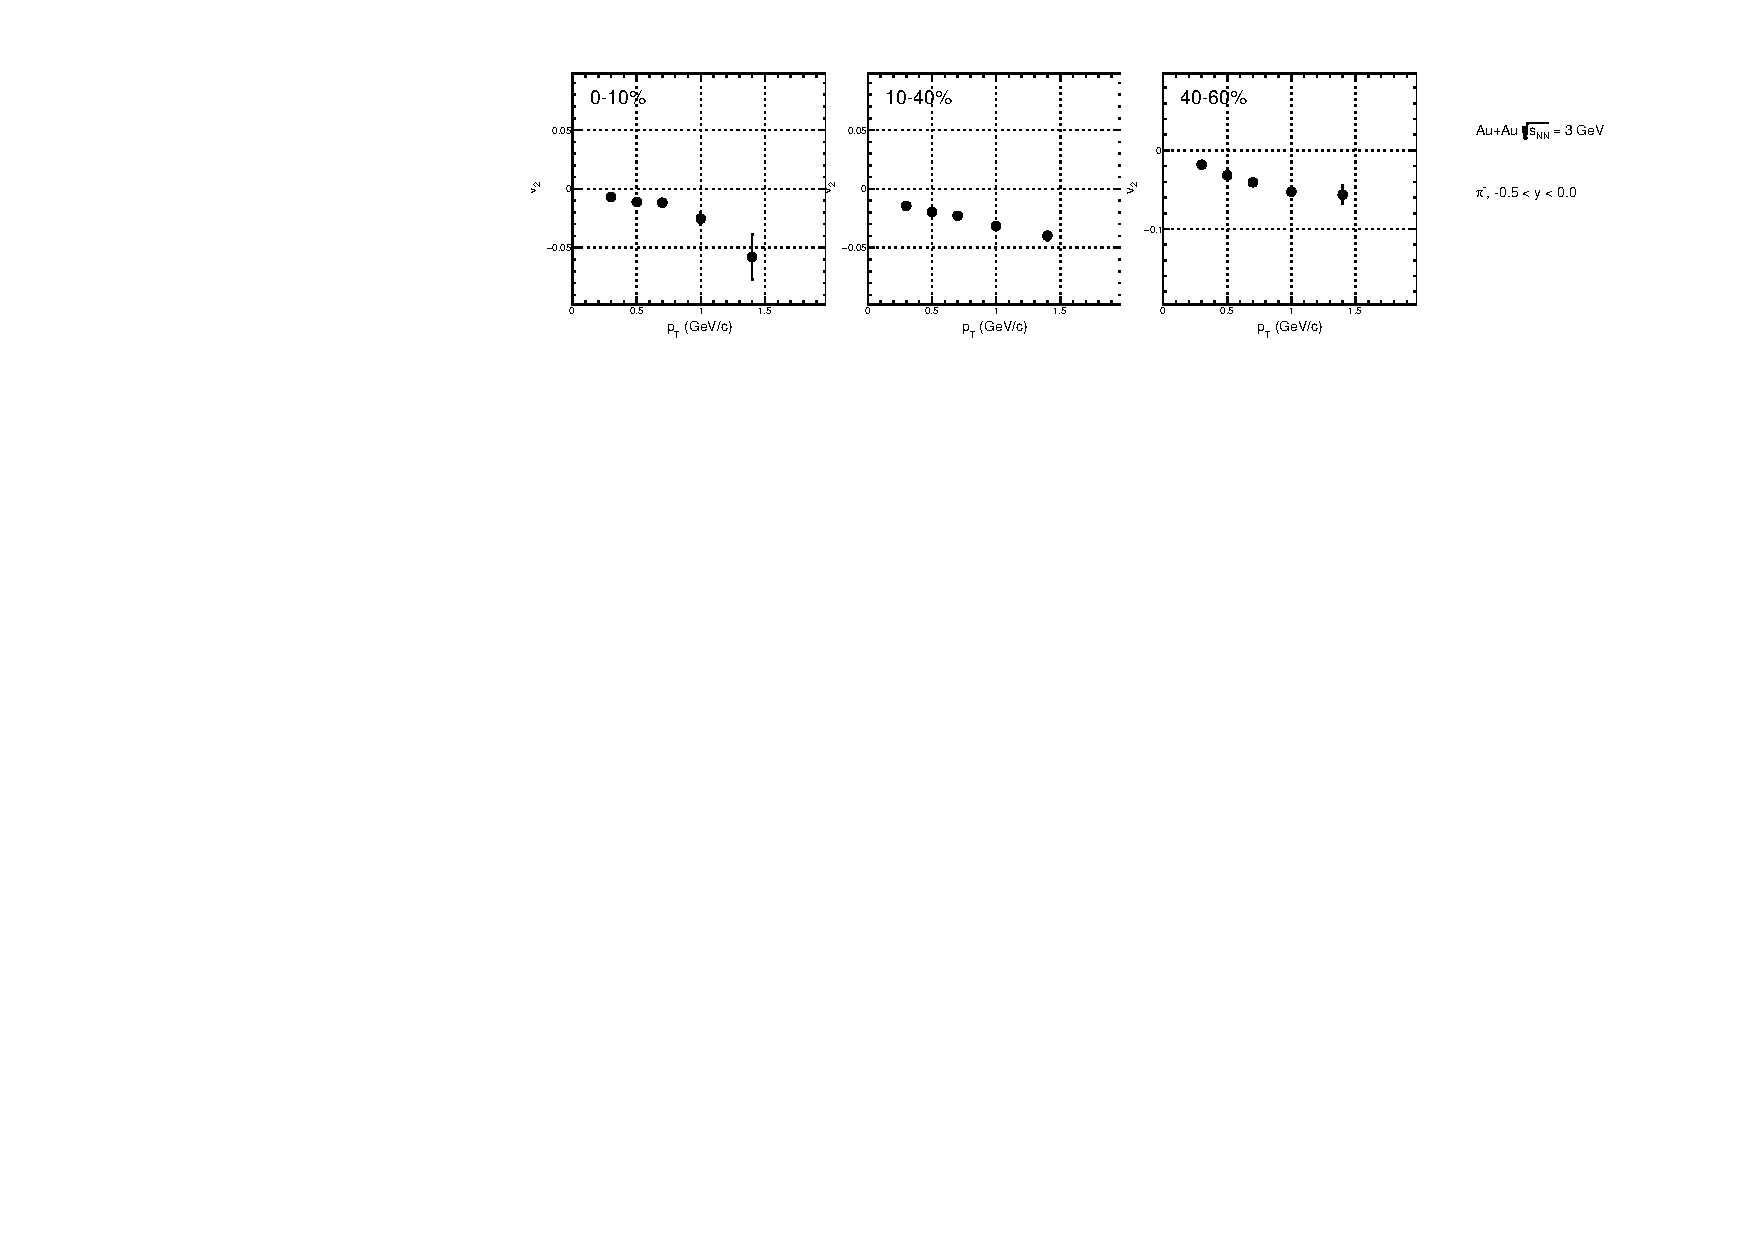
\includegraphics[scale=0.5]{chapter3/fig/v2ptpikp/pionm_v2pt_wide_cent.pdf}
\caption{$v_{2}$ as a function of $p_{T}$ in different centrality bins for $\pi^{+}$ and $\pi^{-}$ in Au+Au collisions at $\sqrt{s_{NN}}$ = 3 GeV in 0-10\%, 10-40\%, 40-60\% centrality bins.}
\label{pion_v2pt_widecent}
\end{figure}



\clearpage


\subsubsection{kaons $v_{2}$ as a function of $p_{T}$ and rapidity}
In this chapter, we will show the results of kaons' $v_{2}$ as a function of $p_{T}$ and rapidity(y).
Figure \ref{kaon_v2y_cent} shows kaon $v_{2}$ as a function of y for different centrality bins from 0-5\% to 50-60\%. The $p_{T}$ range is [0.4, 1.6] GeV/c. Figure \ref{kaon_v2y_widecent} shows the kaons' $v_{2}$ vs. y in wider centrality bin. $K^{+}$ and $K^{-}$ $v_{2}$ are consistent within error bar.



\begin{figure}[h]
\includegraphics[scale=0.4]{chapter3/fig/v2ypikp/v2y_cent_kaonp.pdf}
\includegraphics[scale=0.4]{chapter3/fig/v2ypikp/v2y_cent_kaonm.pdf}
\caption{$v_{2}$ as a function of rapidity(y) in different centrality bins for $K^{+}$ and $K^{-}$ in Au+Au collisions at $\sqrt{s_{NN}}$ = 3 GeV.}
\label{kaon_v2y_cent}
\end{figure}

\begin{figure}[h]
\includegraphics[scale=0.6]{chapter3/fig/v2ypikp/kaonp_v2y_wide_cent.pdf}
\includegraphics[scale=0.6]{chapter3/fig/v2ypikp/kaonm_v2y_wide_cent.pdf}
\caption{$v_{2}$ as a function of rapidity(y) in different centrality bins for $K^{+}$ and $K^{-}$ in Au+Au collisions at $\sqrt{s_{NN}}$ = 3 GeV in 0-10\%, 10-40\%, 40-60\% centrality bins.}
\label{kaon_v2y_widecent}
\end{figure}

We also study the $p_{T}$ dependence for kaons' $v_{2}$ in the figure \ref{kaon_v2pt_cent}, as we can see, kaons' $v_{2}$ is decreasing with $p_{T}$ increasing. Figure \ref{kaon_v2pt_widecent} shows these results in wider centrality bins 0-10\%, 10-40\%, 40-60\%. 


\begin{figure}[h]
\includegraphics[scale=0.5]{chapter3/fig/v2ptpikp/v2pt_cent_kaonp.pdf}
\includegraphics[scale=0.5]{chapter3/fig/v2ptpikp/v2pt_cent_kaonm.pdf}
\caption{$v_{2}$ as a function of $p_{T}$ in different centrality bins for $K^{+}$ and $K^{-}$ in Au+Au collisions at $\sqrt{s_{NN}}$ = 3 GeV.}
\label{kaon_v2pt_cent}
\end{figure}

\begin{figure}[h]
\includegraphics[scale=0.5]{chapter3/fig/v2ptpikp/kaonp_v2pt_wide_cent.pdf}
\includegraphics[scale=0.5]{chapter3/fig/v2ptpikp/kaonm_v2pt_wide_cent.pdf}
\caption{$v_{2}$ as a function of $p_{T}$ in different centrality bins for $K^{+}$ and $K^{-}$ in Au+Au collisions at $\sqrt{s_{NN}}$ = 3 GeV in 0-10\%, 10-40\%, 40-60\% centrality bins.}
\label{kaon_v2pt_widecent}
\end{figure}






\clearpage


\subsubsection{proton $v_{2}$ as a function of $p_{T}$ and rapidity}
In this chapter, we will show the results of protons' $v_{2}$ as a function of $p_{T}$ and rapidity(y).
Figure \ref{proton_v2y_cent} shows proton $v_{2}$ as a function of y for different centrality bins from 0-5\% to 50-60\%. The $p_{T}$ range is [0.4, 2.0] GeV/c. Figure \ref{proton_v2y_widecent} shows the proton’s $v_{2}$ vs. y in wider centrality bin. As we can see, proton $v_{2}$ is negative at mid-rapidity region. In 0-10\% and 10-40\% centrality bin, proton $v_{2}$ is negative at mid-rapidity region, while is positive at forward rapidity region.



\begin{figure}[h]
\includegraphics[scale=0.6]{chapter3/fig/v2ypikp/v2y_cent_proton.pdf}
\caption{proton $v_{2}$ as a function of rapidity(y) in different centrality bins in Au+Au collisions at $\sqrt{s_{NN}}$ = 3 GeV.}
\label{proton_v2y_cent}
\end{figure}

\begin{figure}[h]
\includegraphics[scale=0.6]{chapter3/fig/v2ypikp/protonp_v2y_wide_cent.pdf}
\caption{proton $v_{2}$ as a function of rapidity(y) in different centrality bins for in Au+Au collisions at $\sqrt{s_{NN}}$ = 3 GeV in 0-10\%, 10-40\%, 40-60\% centrality bins.}
\label{proton_v2y_widecent}
\end{figure}

We also study the $p_{T}$ dependence for proton's $v_{2}$ in the figure \ref{proton_v2pt_cent}, as we can see, proton's $v_{2}$ is decreasing with $p_{T}$ increasing. Figure \ref{proton_v2pt_widecent} shows these results in wider centrality bins 0-10\%, 10-40\%, 40-60\%. The proton $v_{2}$ decreases with $p_{T}$ increases, then proton $v_{2}$ increases at higher $p_{T}$ region.


\begin{figure}[h]
\includegraphics[scale=0.6]{chapter3/fig/v2ptpikp/v2pt_cent_proton.pdf}
\caption{proton $v_{2}$ as a function of $p_{T}$ in different centrality bins in Au+Au collisions at $\sqrt{s_{NN}}$ = 3 GeV.}
\label{proton_v2pt_cent}
\end{figure}

\begin{figure}[h]
\includegraphics[scale=0.6]{chapter3/fig/v2ptpikp/protonp_v2pt_wide_cent.pdf}
\caption{proton $v_{2}$ as a function of $p_{T}$ in different centrality bins in Au+Au collisions at $\sqrt{s_{NN}}$ = 3 GeV in 0-10\%, 10-40\%, 40-60\% centrality bins.}
\label{proton_v2pt_widecent}
\end{figure}

\clearpage
\newpage

\subsection{$v_{2}$ from second order event plane}
As discussed in the second chapter, the $v_{2}$ is calculated from first order event plane angle $\Psi_{1}$, this is because the higher first order event plane resolution (up to 70\%) than second order resolution, which will induce the higher lower error bar for $v_{2}$, and numerically it is equivalent to that we use second order event plane angle $\Psi_{2}$ to calculate $v_{2}$. The different order event plane resolution comparison can be found in the figure \ref{res2_tpc_epd}.
Here in the figure \ref{psi2_dis_tpc_epd}, we show the reconstructed second order event plane angle distribution in different centrality in different sub-event group of TPC and EPD. The black line is raw $\Psi_{2}$ distribution, the blue line is $\Psi_{2}$ distribution with re-centering calibration and red line is $\Psi_{2}$ distribution with re-centering and shift calibration,  as we can see, after re-centeringing and shift calibration (the red line) we have flat second order event plane angle $\Psi_{2}$ distribution, and it can be used for $v_{2}$ calculation. 

\begin{figure}[h]
\includegraphics[scale=0.6]{chapter3/fig/second/res_3gev_com.pdf}
\caption{\label{res2_tpc_epd} EPD event plane resolution as a function of collision centrality, the black solid circle is first order event plane resolution, black open circle is the converted second order event plane resolution for $v_{2}$ calculation, the black solid square is second order event plane resolution.}
\end{figure}

\begin{figure}[h]
\includegraphics[scale=0.6]{chapter3/fig/second/psi2.pdf}
\caption{\label{psi2_dis_tpc_epd} TPC and EPD sub-event plane angle ($\Psi_{2}$) distribution in different centralities, the black line is raw $\Psi_{2}$ distribution, the blue line is $\Psi_{2}$ distribution with re-centering calibration, the red line is $\Psi_{2}$ distribution with re-centering and shift calibration.}
\end{figure}

We calculate the proton $v_{2}$ as a function of $p_{T}$ using second order event plane angle $\Psi_{2}$ and make comparison to the results from using first order event plane angle. It can be found in the figure \ref{v2pt_sec_com}. We found their results are consistent in the low $p_{T}$ and middle $p_{T}$ region. There is little difference in the high $p_{T}$ region, we think this could be some effect from proton's purity, and the error is also too large. So far, our conclusion is that the results of $v_{2}$ using first order and second event plane angle are consistent.

\begin{figure}[h]
\includegraphics[scale=0.6]{chapter3/fig/second/v2pt_com.pdf}
\caption{\label{v2pt_sec_com} $v_{2}$ as a function of $p_{T}$ in 3GeV Au+Au collisions, 10-40\% centrality from first order and second event plane angle, and their ratio.}
\end{figure}

In order to confirm this, we also do the same analysis (calculate $v_{2}$ using first order and second order event plane angle) using UrQMD model. First, we show the resolution of different order event plane in the figure \ref{urqdm_res2}, we have the same conclusion with data, the second order event plane resolution is quite small than first order event plane resolution, which will induce larger error bar when calculating $v_{2}$. In the figure \ref{v2pt_urqmd_com}, we calculate the $v_{2}$ from first order and second event plane angle and make comparison. 
We found they are consistent within the error bar.

\begin{figure}[h]
\includegraphics[scale=0.6]{chapter3/fig/second/res_urqmd.pdf}
\caption{\label{urqmd_res2} The event plane resolution as a function collision centrality at 3GeV in UrQMD model for first order second order and converted second order.}
\end{figure}

\begin{figure}[h]
\includegraphics[scale=0.6]{chapter3/fig/second/v2pt_urqdm.pdf}
\caption{\label{v2pt_urqmd_com} $v_{2}$ as a function of $p_{T}$ at 3 GeV 10-40\% in UrQMD model from first order and second event plane angle, and their ratio.}
\end{figure}


\clearpage
\subsection{Systematic Uncertainties}

Point-by-point systematic errors on variables used for tracks cuts and particle identification and resolution. For all systematic checks, the various cuts are changed one at a time. Table \ref{sys_cut_pionkaon} shows the systematic cuts and minimum and maximum values used in the analysis for pions and kaons. Similarly, table \ref{sys_cut_proton} shows the systematic cuts used in the analysis for proton. 
For each cut variable, we choose the maximum deviation from default value, then the total systematic uncertainty can be estimated using in the equation \ref{sys_equation} from different source (dca, nHitsFit, n$\sigma_{particle}$, resolution, efficiency). The systematic uncertainty contribution from resolution should be constants for each particle in fine centrality bin. While there will be difference in wide centrality bin(10-40\%) because the relative number of particles in fine centrality bin are not same for each particle species. But in this analysis, the  

\begin{equation}
	sys_{total}=\sqrt{(y_{dca}-y_{def})^{2} + (y_{nHit}-y_{def})^{2} + (y_{n\sigma}-y_{def})^{2} + (y_{EP}-y_{def})^{2} + (y_{eff}-y_{def})^{2}}
\label{sys_equation}
\end{equation}

\begin{table}[ht]
\caption{Systematic cuts for pions and kaons}
\label{sys_cut_pionkaon}
\begin{tabular}{cccc}
\hline
Cuts & Default & var1 & var2\\ 
\hline
dca ($<$) & 3 & 1 & 2\\ 
%\hline
nHitFit ($>$) & 15 & 10 & 20\\ 
%\hline
$|$ n$\sigma_{particle}$ $|$ $<$ & 3 & 2 & 2.5 \\ 
%\hline
resolution reference EP & EPD-C & EPD-CD & EPD D\\ 
\hline
\end{tabular} 
\end{table}


\begin{table}[ht]
\caption{Systematic cuts for proton}
\label{sys_cut_proton}
\begin{tabular}{cccc}
\hline
Cuts & Default & var1 & var2\\ 
\hline
dca ($<$) & 3 & 1 & 2\\ 
%\hline
nHitFit ($>$) & 15 & 10 & 20\\ 
%\hline
$|$ n$\sigma_{particle}$ $|$ $<$ & 2 & 3 & 2.5 \\ 
%\hline
resolution reference EP & EPD-C & EPD-CD & EPD D\\ 
\hline
\end{tabular} 
\end{table}

\begin{figure}[h]
\includegraphics[scale=0.5]{chapter3/fig/sys/pion/v1y_pip_sys.pdf}
\includegraphics[scale=0.5]{chapter3/fig/sys/pion/v1y_pim_sys.pdf}
\caption{Systematic uncertainty study for $v_{1}$ as a function of rapidity in 10-40\% for pion at $\sqrt{s_{NN}}$ = 3 GeV. Left is $v_{1}$ as a function of rapidity from different cut, right is fitted results of $dv_{1}/dy$ from different source cut .}
\label{pion_v1y_sys}
\end{figure}

\begin{figure}[h]
\includegraphics[scale=0.4]{chapter3/fig/sys/pion/v2y_pip_sys.pdf}
\includegraphics[scale=0.4]{chapter3/fig/sys/pion/v2y_pim_sys.pdf}
\caption{Systematic uncertainty study for $v_{2}$ as a function of rapidity in 10-40\% for pion at $\sqrt{s_{NN}}$ = 3 GeV.}
\label{pion_v1y_sys}
\end{figure}

\begin{figure}[h]
\includegraphics[scale=0.4]{chapter3/fig/sys/pion/v1pt_pip_sys.pdf}
\includegraphics[scale=0.4]{chapter3/fig/sys/pion/v1pt_pim_sys.pdf}
\caption{Systematic uncertainty study for $v_{1}$ as a function of $p_{T}$ in 10-40\% for pion at $\sqrt{s_{NN}}$ = 3 GeV}
\label{pion_v1y_sys}
\end{figure}

\begin{figure}[h]
\includegraphics[scale=0.4]{chapter3/fig/sys/pion/v2pt_pip_sys.pdf}
\includegraphics[scale=0.4]{chapter3/fig/sys/pion/v2pt_pim_sys.pdf}
\caption{Systematic uncertainty study for $v_{2}$ as a function of $p_{T}$ in 10-40\% for pion at $\sqrt{s_{NN}}$ = 3 GeV.}
\label{pion_v1y_sys}
\end{figure}


\begin{figure}[h]
\includegraphics[scale=0.5]{chapter3/fig/sys/kaon/v1y_kp_sys.pdf}
\includegraphics[scale=0.5]{chapter3/fig/sys/kaon/v1y_km_sys.pdf}
\caption{Systematic uncertainty study for $v_{1}$ as a function of rapidity in 10-40\% for kaon at $\sqrt{s_{NN}}$ = 3 GeV. Left is $v_{1}$ as a function of rapidity from different cut, right is fitted results of $dv_{1}/dy$ from different source cut .}
\label{pion_v1y_sys}
\end{figure}

\begin{figure}[h]
\includegraphics[scale=0.4]{chapter3/fig/sys/kaon/v2y_kp_sys.pdf}
\includegraphics[scale=0.4]{chapter3/fig/sys/kaon/v2y_km_sys.pdf}
\caption{Systematic uncertainty study for $v_{2}$ as a function of rapidity in 10-40\% for kaon at $\sqrt{s_{NN}}$ = 3 GeV.}
\label{pion_v1y_sys}
\end{figure}

\begin{figure}[h]
\includegraphics[scale=0.4]{chapter3/fig/sys/kaon/v1pt_kp_sys.pdf}
\includegraphics[scale=0.4]{chapter3/fig/sys/kaon/v1pt_km_sys.pdf}
\caption{Systematic uncertainty study for $v_{1}$ as a function of $p_{T}$ in 10-40\% for kaon at $\sqrt{s_{NN}}$ = 3 GeV}
\label{pion_v1y_sys}
\end{figure}

\begin{figure}[h]
\includegraphics[scale=0.4]{chapter3/fig/sys/kaon/v2pt_kp_sys.pdf}
\includegraphics[scale=0.4]{chapter3/fig/sys/kaon/v2pt_km_sys.pdf}
\caption{Systematic uncertainty study for $v_{2}$ as a function of $p_{T}$ in 10-40\% for kaon at $\sqrt{s_{NN}}$ = 3 GeV.}
\label{pion_v1y_sys}
\end{figure}


\begin{figure}[h]
\includegraphics[scale=0.5]{chapter3/fig/sys/proton/v1y_pp_sys.pdf}
\caption{Systematic uncertainty study for $v_{1}$ as a function of rapidity in 10-40\% for proton at $\sqrt{s_{NN}}$ = 3 GeV. Left is $v_{1}$ as a function of rapidity from different cut, right is fitted results of $dv_{1}/dy$ from different source cut .}
\label{pion_v1y_sys}
\end{figure}

\begin{figure}[h]
\includegraphics[scale=0.4]{chapter3/fig/sys/proton/v2y_pp_sys.pdf}
\caption{Systematic uncertainty study for $v_{2}$ as a function of rapidity in 10-40\% for proton at $\sqrt{s_{NN}}$ = 3 GeV.}
\label{pion_v1y_sys}
\end{figure}

\begin{figure}[h]
\includegraphics[scale=0.4]{chapter3/fig/sys/proton/v1pt_pp_sys.pdf}
\caption{Systematic uncertainty study for $v_{1}$ as a function of $p_{T}$ in 10-40\% for proton at $\sqrt{s_{NN}}$ = 3 GeV}
\label{pion_v1y_sys}
\end{figure}

\begin{figure}[h]
\includegraphics[scale=0.4]{chapter3/fig/sys/proton/v2pt_pp_sys.pdf}
\caption{Systematic uncertainty study for $v_{2}$ as a function of $p_{T}$ in 10-40\% for proton at $\sqrt{s_{NN}}$ = 3 GeV.}
\label{pion_v1y_sys}
\end{figure}


















%Results
\clearpage
\section{Discussion} 
In this chapter, we will review the results of number of constituent quark scaling of elliptic for identified particles from STAR BES-I and compare with the results that from 3 GeV to discuss the partonic collectivity at RHIC-STAR energy region.  The $p_{T}$ integrated $v_{2}$ will also be discussed and compared with world data. The excitation function indicates the elliptic flow evolves from a in-plane flow ($v_{2} > 0$) to an out-of-plane flow pattern as the collision energy decreases due to the shadowing effect from spectators. The directed flow slope of identified particle will be discussed and compared with the higher energy from STAR BES-I. 

\subsection{Development of elliptic flow}
In non-central heavy ion collisions, the overlap region of colliding nuclei is like almond-shaped. This spatial anisotropy will cause larger pressure gradients in the direction of participant plane compared to out of this plane, which finally result in azimuthal anisotropy of the momenta of the produced particles. The elliptic flow $v_{2}$ is the second harmonic coefficient of the Fourier decomposition of the azimuthal particle distribution with respect to event plane.

At high energy, the passage time of the projectile and target spectators is much smaller than the development time of medium expansion. The passage time is $ \sim 2R/(\gamma_{0} v_{0})$, where R is the nuclear radius, $v_{0}$ is the spectator velocity in the CM frame. The development time of medium expansion can be estimated as $\sim$ $R/c_{s}$, where the speed of sound $c_{s} = \sqrt{\partial p/\partial e}$, where the p is the pressure, and e is the energy density. The spectators will have little effect on the medium expansion at high energy. When the collision energy decreases, the passage time of spectators might be larger than the development time of medium expansion. This will cause shadowing of "squeeze-out" effect by spectators. It means the spectators shadow the expansion of medium alone impact parameter direction, which leads to negative elliptic flow \cite{Pinkenburg:1999ya}. This is important for understanding the equation of state (EoS) at low energy \cite{Danielewicz:1998vz, Danielewicz:2002pu}.

\subsection{Number of constituent quark scaling of elliptic flow ($v_{2}$)}
Quark coalescence and recombination mechanisms ~\cite{Fries:2003vb,Hwa:2003bn} in particle production for heavy-ion collisions predict that if particles are made up of quarks then the elliptic flow $v_{2}(p_{T})$ of the particles will scale with their number of constituent quarks and follow a universal trend ~\cite{Molnar:2003ff} . The number of constituent quark for meson is two, for baryon is three. It is always performed as $v_{2}$ divide by number of consistent quark ($n_{q}$) for various particle species as a function of $(m_{T}-m_{0})/n_{q}$. Here the transport mass $m_{T}$ is defined as $m_{T} = \sqrt{p_{T}^{2}+m_{0}^{2}}$. The variable transverse kinetic energy is chosen in order to remove particle mass dependence from the flow coefficients.  The number of constituent quark scaling for elliptic flow has been argued for a evidence for partonic degree of freedom.

From STAR previous measurements, the identified hadrons follow a universal scaling at top BES-I energy 200 GeV, which indicates the light quark (u, d, s) even charm quark (c) exhibit the same strong collective behavior and may be close to thermal equilibrium in Au+Au collisions at 200 GeV ~\cite{Abelev:2008ae, Adamczyk:2015ukd, Adamczyk:2017xur}. While at lower STAR BES-I energy region, the difference of elliptic flow between particle and anti-particle have been observed, especially for the baryons. The difference is increasing with collision energy decreasing ~\cite{Adamczyk:2013gv}. This indicates the break of NCQ scaling between particles and antiparticles. Many theoretical calculation or transport model ~\cite{Dunlop:2011cf, Steinheimer:2012bn, Sun:2014rda, Hatta:2015era, Xu:2013sta} study this effect and have a description of pion, kaon and proton $v_{2}$ difference. The individual positive and negative charged hadrons still have good NCQ scaling when collision energy is larger than 19.6 GeV \cite{Adamczyk:2013gw}. At 7.7 GeV, we still have NCQ scaling within 10\% uncertainty. From STAR recent publication, the pion and proton $v_{2}$ follow same trend within statistics errors at 4.5 GeV~\cite{Adam:2020pla}. We would like to ask whether the partonic phase developed and how the NCQ scaling behave at $\sqrt{s_{NN}}$ = 3 GeV.

Fig \ref{fig:v2pt_ncq} shows the number of constituent scaled $v_{2}$ as a function of transverse kinetic energy in 10-40\% centrality. The data points are from STAR run18 54.4GeV and FXT 3GeV, and run19 27GeV, pion, kaon, proton $v_{2}$ results. The different color dash lines represent the fit to data from 200-3 GeV, in order to strength the scaled $v_{2}$ at different energy \cite{Dong:2004ve}, they can be found in Figure\ref{fig:v2pt_ncq_fit}. As we can see at 27 and 54.4 GeV, the NCQ scaling of individual positive and negative particles holds well, which is consistent with that the elliptic flow is driven by partonic collectivity. While at 3 GeV, we found different behavior of $v_{2}$. By comparing to the data from 4.5 GeV, we found the measured $v_{2}$ for all particles are negative and the NCQ scaling is absent, especially for positive charged particles. This significant change from 4.5GeV to 3GeV indicates new medium properties produced at 3GeV that are different from the partonic matter created in high energy collisions. 

\begin{figure}[h]
\includegraphics[scale=0.6]{FXT3gev/chapter4/fig/v2pt_ncq.pdf}
\caption{Number of constituent quark scaled $v_{2}$ for pion, kaon and proton as a function of scaled transverse kinetic energy in 10-40\% at 3, 27 and 54.4 GeV for positive charged particles (a) and negative charged particles (b). Different color dash line indicates the strength of scaled $v_{2}$ at different collision energy from fitting.}
\label{fig:v2pt_ncq}
\end{figure}

\begin{figure}
    \centering
    \includegraphics[scale=0.7]{FXT3gev/chapter4/fig/v2ncq_energy.pdf}
    \includegraphics[scale=0.5]{FXT3gev/chapter4/fig/lam_ks0_v2ncq.pdf}
    \includegraphics[scale=0.25]{FXT3gev/chapter4/fig/4_5GeV_ncq.pdf}
    \caption{Fitting to STAR data from 200-4.5 GeV in 10-40\% centrality.}
    \label{fig:v2pt_ncq_fit}
\end{figure} 

\clearpage
\newpage

\subsection{$p_{T}$ integrated $v_{2}$}

In order to compare the $p_{T}$ integrated $v_{2}$ at 3GeV with world data. In this chapter, we talk about the calculation of $p_{T}$ integrated $v_{2}$.

The $p_{T}$ integrated $v_{2}$, is also average $v_{2}$, over certained $p_{T}$ region. We denote the average $v_{2}$ as $<v_{2}>$, it can be calculated using formula \ref{ave_v2}. Where the $dN/dp_{T}$ is the transverse momentum distribution and $v_{2}(p_{T})$ is measured differential $v_{2}$ as a function of $p_{T}$. Weighting by the number of particles, we can calculate the average $v_{2}$ ($<v_{2}>$) in the centained $p_{T}$ range.

\begin{equation}
    <v_{2}> = \frac{\sum_{i} dN^{i}/dp_{T}*v_{2}^{i}(p_{T})}{\sum_{i}dN^{i}/dp_{T}}
    \label{ave_v2}
\end{equation}

Figure \ref{fig:dndpt_v2pt_proton} shows the proton $dN/dp_{T}$ distribution and differential $v_{2}$ as a function of $p_{T}$ in 10-40\% at 3GeV. From these distribution associated with formula \ref{ave_v2}, we can calculate proton $<v_{2}>$ in $p_{T}$ range [0.4,2.0] GeV/c and apply the same procedure to calculate $\pi^{\pm}$ $<v_{2}>$ in the $p_{T}$ range [0.2, 1.6] GeV/c.

Figure \ref{fig:v2_energy} shows the measured $p_{T}$ integrated $v_{2}$ as a function of collision energy. The STAR data points are proton and pion $v_{2}$ from BES-I energy 10-40\% and 4.5GeV 0-30\% \cite{Adam:2020pla}. The other data points shown are from FOPI \cite{Andronic:2004cp}, E895 \cite{Pinkenburg:1999ya}, and E877 \cite{Voloshin:1997rs}. As we can see, the new results at 3GeV from STAR are well agree with world data trend.

\begin{figure}
    \centering
    \includegraphics[scale=0.6]{FXT3gev/chapter4/fig/v2integral_proton.pdf}
    \caption{(Left) $dN/dp_{T}$ distribution for proton in 10-40\%. (Right) Differential $v_{2}$ as a function of $p_{T}$ for proton in 10-40\%.}
    \label{fig:dndpt_v2pt_proton}
\end{figure}

\begin{figure}
    \centering
    \includegraphics[scale=0.5]{FXT3gev/chapter4/fig/v2_energy.pdf}
    \caption{$p_{T}$ integrated $v_{2}$ for proton, pion or Z=1 hadrons as a function of collision energy. The STAR data point are proton and pion $v_{2}$ from BES-I 10-40\%, and 4.5GeV 0-30\%, and 3GeV 10-40\%. The other data are shown from FOPI, E985, E877.}
    \label{fig:v2_energy}
\end{figure}

\clearpage
\newpage
\subsection{Directed flow measurements}

Directed flow measurement of identified particles from STAR has been performed from 200GeV down to 4.5GeV \cite{Adamczyk:2014ipa, Adamczyk:2017nxg, Adam:2020pla}. The non-monotonic collision energy dependence proton  directed flow has been argued for a evidence of softenest point of equation of state \cite{Hung:1994eq, Konchakovski:2014gda, Nara:2016phs}. While other particle's $v_{1}$ are all negative. From previous AGS E895 measurements of proton directed flow $v_{1}$, we know the proton and $\Lambda$ $v_{1}$ are positive when collision energy $\sqrt{s_{NN}} <$ 10GeV and increase with collision energy decreases \cite{Liu:2000am}.  

In this analysis at 3GeV, we present $\pi^{\pm}, K^{\pm}, K^{0}_{S}, proton, \Lambda, \phi$ $v_{1}$ in 10-40\% centrality and compared to that from STAR high energy
 in figure \ref{fig:v1_energy}, As we can see, the proton and $\Lambda$ results are consistent with the energy trend and pions $v_{1}$ stays negative. But for the first time that the kaon and $\phi$ $v_{1}$ are found to be positive which is consistent with a change of equation of state. At 3Gev, it has been reached to high baryon density region, the $K^{+}$ will be associated production with $\Lambda$ and might follow collective behavior with $\Lambda$.


\begin{figure}
    \centering
    \includegraphics[scale=0.5]{FXT3gev/chapter4/fig/v1_energy.pdf}
    \caption{Collision energy dependence of directed flow $v_{1}$ slope for pion, kaon, proton, $\Lambda$ and $\phi$ in 10-40\% or 10-30\% from STAR.} 
    \label{fig:v1_energy}
\end{figure}

\subsection{Combination Results}

In this analysis, the $v_1$ results between positive and negative particle are combined for both pions and kaons, as the difference among them are very small. 
The method for combining these results are listed below: firstly the weight factor is calculated by the inverse of statistics error square. Then we combined results and error are calculated by weighting the weight factor, the similar way for kaons analysis.

\begin{equation}
    w (\pi^{+}) = \frac{1}{error_{stat}(\pi^{+})} \qquad
    w (\pi^{-}) = \frac{1}{error_{stat}(\pi^{-})}
\end{equation}

\begin{equation}
    v_{1}(\pi) = \frac{v_{1}(\pi^{+})*w(\pi^{+}) + v_{1}(\pi^{-})*w(\pi^{-})}{w(\pi^{+})+w(\pi^{-})}
\end{equation}
\begin{equation}
    error_{stat}(\pi) = \sqrt{1/(w(\pi^{+})+w(\pi^{-}))}
\end{equation}
\begin{equation}
    error_{sys}(\pi) = \frac{error_{sys}(\pi^{+})*w(\pi^{+}) + error_{sys}(\pi^{-})*w(\pi^{-})}{w(\pi^{+})+w(\pi^{-})}
\end{equation}



















%Analysis Techniques
\clearpage
\section{$K^0_S$ and $\Lambda$ analysis} 
\subsection{Particle reconstruction}
\subsection{Acceptance and efficiency}
\subsubsection{Acceptance}

\begin{figure}[h]
\includegraphics[width=0.49\linewidth]{chapterX/fig/ks_acceptance_v15.pdf}
\includegraphics[width=0.49\linewidth]{chapterX/fig/ld_acceptance_v15.pdf}
\caption{Acceptance of $K^0_S$(left) and $\Lambda$(right) for $10-40\%$ centrality at $\sqrt{s_{NN}}$ = 3 GeV.}
\label{ldks_acceptance}
\end{figure}



\subsubsection{Efficiency corrections}

\begin{figure}[h]
\includegraphics[width=0.49\linewidth]{chapterX/fig/ks_efficiency_v15.pdf}
\includegraphics[width=0.49\linewidth]{chapterX/fig/ld_efficiency_v15.pdf}
\caption{Reconstruction efficiency of $K^0_S$(left) and $\Lambda$(right), as a function of $y$ and $p_{\rm{T}}$ for $10-40\%$ centrality at $\sqrt{s_{NN}}$ = 3 GeV.}
\label{ldks_acceptance}
\end{figure}


\subsection{$v_1$ and $v_2$ extraction}
\subsection{Systematic uncertainties}
\subsubsection{$v_1$}

\begin{figure}[h]
\includegraphics[width=0.49\linewidth]{chapterX/fig/ks_sys_cut_v1.pdf}
\includegraphics[width=0.49\linewidth]{chapterX/fig/ks_sys_cut_v1_nhits.pdf}
\includegraphics[width=0.49\linewidth]{FXT3gev/chapterX/fig/ks_sys_cut_v1_msigma.pdf}
\includegraphics[width=0.49\linewidth]{FXT3gev/chapterX/fig/ks_sys_cut_v1_epdres.pdf}
\caption{Systematic uncertainty study for $v_{1}$ as a function of rapidity in 10-40\% for $K^0_S$ at $\sqrt{s_{NN}}$ = 3 GeV.}
\label{ks_v1y_sys}
\end{figure}

\begin{figure}[h]
\includegraphics[width=0.49\linewidth]{chapterX/fig/ks_sys_cut_vn.pdf}
\includegraphics[width=0.49\linewidth]{chapterX/fig/ks_sys_cut_vn_nhits.pdf}
\includegraphics[width=0.49\linewidth]{FXT3gev/chapterX/fig/ks_sys_cut_vn_msigma.pdf}
\includegraphics[width=0.49\linewidth]{FXT3gev/chapterX/fig/ks_sys_cut_vn_epdres.pdf}
\caption{Systematic uncertainty study for $dv_{1}/dy$ as a function of centrality for $K^0_S$ at $\sqrt{s_{NN}}$ = 3 GeV.}
\label{ks_dv1dy_sys}
\end{figure}

\begin{figure}[h]
\includegraphics[width=0.49\linewidth]{chapterX/fig/ld_sys_cut_v1.pdf}
\includegraphics[width=0.49\linewidth]{chapterX/fig/ld_sys_cut_v1_nhits.pdf}
\includegraphics[width=0.49\linewidth]{FXT3gev/chapterX/fig/ld_sys_cut_v1_msigma.pdf}
\includegraphics[width=0.49\linewidth]{FXT3gev/chapterX/fig/ld_sys_cut_v1_epdres.pdf}
\caption{Systematic uncertainty study for $v_{1}$ as a function of rapidity in 10-40\% for $\Lambda$ at $\sqrt{s_{NN}}$ = 3 GeV.}
\label{lambda_v1y_sys}
\end{figure}

\begin{figure}[h]
\includegraphics[width=0.49\linewidth]{chapterX/fig/ld_sys_cut_vn.pdf}
\includegraphics[width=0.49\linewidth]{chapterX/fig/ld_sys_cut_vn_nhits.pdf}
\includegraphics[width=0.49\linewidth]{FXT3gev/chapterX/fig/ld_sys_cut_vn_msigma.pdf}
\includegraphics[width=0.49\linewidth]{FXT3gev/chapterX/fig/ld_sys_cut_vn_epdres.pdf}
\caption{Systematic uncertainty study for $dv_{1}/dy$ as a function of centrality for $\Lambda$ at $\sqrt{s_{NN}}$ = 3 GeV.}
\label{lambda_dv1dy_sys}
\end{figure}



\subsubsection{$v_2$}

\begin{figure}[h]
\includegraphics[width=0.49\linewidth]{chapterX/fig/ks_sys_cut_v2.pdf}
\includegraphics[width=0.49\linewidth]{chapterX/fig/ks_sys_cut_v2_nhits.pdf}
\includegraphics[width=0.49\linewidth]{FXT3gev/chapterX/fig/ks_sys_cut_v2_msigma.pdf}
\includegraphics[width=0.49\linewidth]{FXT3gev/chapterX/fig/ks_sys_cut_v2_epdres.pdf}
\caption{Systematic uncertainty study for $v_{2}$ as a function of rapidity in 10-40\% for $K^0_S$ at $\sqrt{s_{NN}}$ = 3 GeV.}
\label{ks_v1y_sys}
\end{figure}




\begin{figure}[h]
\includegraphics[width=0.49\linewidth]{chapterX/fig/ld_sys_cut_v2.pdf}
\includegraphics[width=0.49\linewidth]{chapterX/fig/ld_sys_cut_v2_nhits.pdf}
\includegraphics[width=0.49\linewidth]{FXT3gev/chapterX/fig/ld_sys_cut_v2_msigma.pdf}
\includegraphics[width=0.49\linewidth]{FXT3gev/chapterX/fig/ld_sys_cut_v2_epdres.pdf}
\caption{Systematic uncertainty study for $v_{2}$ as a function of rapidity in 10-40\% for $\Lambda$ at $\sqrt{s_{NN}}$ = 3 GeV.}
\label{lambda_v2y_sys}
\end{figure}




\subsection{Results}
\subsubsection{$v_1$ results for $K^0_S$, $\Lambda$}

\begin{figure}[h]
\includegraphics[width=0.49\linewidth]{chapterX/fig/ks_sys_v1.pdf}
\includegraphics[width=0.49\linewidth]{chapterX/fig/ks_sys_vn.pdf}
\caption{$v_1$ as a function of rapidity(left) for $10-40\%$ centrality and  $dv_{1}/dy$ as a function of centrality(right) for $K^{0}_{S}$ at $\sqrt{s_{NN}}$ = 3 GeV.}
\label{ks_dv1dy_sys}
\end{figure}

\begin{figure}[h]
\includegraphics[width=0.49\linewidth]{chapterX/fig/ld_sys_v1.pdf}
\includegraphics[width=0.49\linewidth]{chapterX/fig/ld_sys_vn.pdf}
\caption{$v_1$ as a function of rapidity(left) for $10-40\%$ centrality and  $dv_{1}/dy$ as a function of centrality(right) for $\Lambda$ at $\sqrt{s_{NN}}$ = 3 GeV.}
\label{lambda_dv1dy_sys}
\end{figure}


\subsubsection{$v_2$ results for $K^0_S$, $\Lambda$}

\begin{figure}[h]
\includegraphics[width=0.49\linewidth]{chapterX/fig/ks_sys_v2.pdf}
\includegraphics[width=0.49\linewidth]{chapterX/fig/ld_sys_v2.pdf}
\caption{$K^0_S$(left) and $\Lambda$(right) $v_2$ as a function of rapidity for $10-40\%$ centrality at $\sqrt{s_{NN}}$ = 3 GeV. For $K^0_S$, the forward rapidity is reflected to compare with the backward rapidity result.}
\label{ks_dv1dy_sys}
\end{figure}



\begin{figure}[h]
\includegraphics[width=0.32\linewidth]{chapterX/fig/q_v2_k_pt.pdf}
\includegraphics[width=0.32\linewidth]{chapterX/fig/q_v2_k_pt_check.pdf}
\includegraphics[width=0.32\linewidth]{chapterX/fig/data_v2_ld_pt.pdf}
\caption{$K^0_S$(left, middle) and $\Lambda$(right) $v_2$ as a function of $p_{T}$ in different rapidity ranges for $10-40\%$ centrality at $\sqrt{s_{NN}}$ = 3 GeV. The results are compared with protons and charged kaons.}
\label{ldks_dv2dpt}
\end{figure}


\begin{figure}[h]
\includegraphics[width=0.80\linewidth]{chapterX/fig/data_v2_ld_ks_mt.pdf}
\caption{$K^0_S$ and $\Lambda$(right) $v_2/q$ as a function of $(m_{T}-m_{0})/n_{q}$ at mid-rapidity for $10-40\%$ centrality at $\sqrt{s_{NN}}$ = 3 GeV. The results are compared with protons and charged kaons.}
\label{ldks_dv2dmt}
\end{figure}
%Lambda, K_S
\clearpage

\bibliography{bib}
%\end{thebibliography}

\clearpage

%\appendix
%\input{Appendix/A}

%\bibliographystyle{plain}

%\bibliographystyle{plain}




\end{document}
